\documentclass{article}
\usepackage[utf8]{inputenc}
\usepackage{fullpage,enumitem,amsmath,amssymb,graphicx, caption, hyperref}

\hypersetup{
    colorlinks=true,
    linkcolor=blue,
    filecolor=magenta,   
    urlcolor=cyan,
}

\numberwithin{equation}{section}

\title{Research Notes on Self-Coupled Spiking Neural Networks}
\author{Chris Fritz}
\date{July 2020}

\begin{document}

\maketitle


\tableofcontents 
\clearpage

\section{The self-coupled SNN Model}

\textit{\textbf{Problem Statement}}
\\
\\
 Given:

\begin{itemize}
    \item A Linear Dynamical System  $\frac{dx}{dt} = A x(t) + B c(t)$,  $x \in \mathbf{R}^d$
    
    \item A Decoder Matrix $D \in \mathbf{R}^{d\hspace{1mm} \times \hspace{1mm}N}$ specifying the preferred directions of N neurons in d-dimensional space,
    
\end{itemize}
synthesize a spiking neural network that implements the linear dynamical system.   
\\
\\
\\
\textbf{\textit{Features}}
\\
\begin{enumerate}
    \item \textbf{\textit{Long-Term Network Accuracy}} The Deneve network assumes $\hat{x}=x$. We show this assumption produces estimation error between the network and its target system that increases with time. By avoiding this assumption, the self-coupled network remains accurate over time. 
    
    \item \textbf{\textit{Tuning Curve Rotation}} To most efficiently use neurons, we use orthogonal coding directions via SVD. The dynamics matrix $A$ is diagonalized by an orthonormal basis $\mathcal{U}$ in d-dimensional space, while the decoder matrix $D$ is chosen such that $\mathcal{U}$ gives its left singular vectors. This choice of coding directions eliminates the need for coupling. 
    
 	    
	At least two neurons per dimension (2d in total) are required since voltage thresholds are strictly positive.
    N-neuron ensembles can thus represent systems with $\frac{N}{2}$ dimensions or less. 
    
    \item \textbf{\textit{Post-synaptic Spike Dropping}} At each synapse, neurotransmitter release due to an action potential is probabilistic.  We incorporate probabilistic spike transmission by thinning at every synaptic connection. The pre-synaptic neuron's membrane potential is still deterministically reset by an action potential. 
    
    \item \textbf{\textit{Dimensionless Time}} We describe both the network and target system in dimensionless time. Time is normalized by the synapses' time constant, $\tau_s$. This dimensionless representation ensures consistent numerical simulation independent of simulation timestep. Furthermore, $\tau_s$ is implicitly specified as 1, reducing the model's parameters by one.     
\end{enumerate}


\clearpage

\section{Derivation of the Basic Model}
\label{section:derivation:basic_model}
\subsection{Predecessor: PCF Voltage Dynamics}
\begin{enumerate}
    \item Let $\tau_s$ be the synaptic time constant of each synapse in the network. Define dimensionless time as:
    \begin{equation*}
        \xi \overset{\Delta}{=} \frac{t}{\tau_s}.
    \end{equation*}\\
    We now assume our Linear Dynamical System is expressed in dimensionless time, i.e
    
    \begin{equation}
        \label{eq:lds_dimensionless}
        \frac{dx}{d\xi} = Ax(\xi) + B c(\xi).
    \end{equation}
    
    To describe the neuron dynamics in dimensionless time, let $o(\xi) \in \mathbf{R}^{N}$ be the spike trains of N neurons composing the network with components
    \begin{equation*}
        o_j(\xi) = \sum_{k=1}^{\text{$n_j$ spikes}} \delta(\xi - \xi_{j}^{k}),
    \end{equation*}
    where $\xi_j^k$ is the time at which neuron $j$ makes its $k^{th}$ spike. 
    Define the network's estimate of the state variable as
    \begin{equation}
        \label{eq:xhat}
        \hat{x}(\xi)
        \overset{\Delta}{=} D r(\xi), 
    \end{equation}
    where $D \in \mathbf{R}^{d \times N}$ and 
    \begin{equation}
    \label{eq:rdot}
        \frac{dr}{d \xi} = -r + o(\xi).
    \end{equation}\\
    When the probability of synaptic transmission is $1$, component $r_j$ is the total received post-synaptic current (PSC) from neuron $j$ by the network estimator. 
    Define the network error as
    \begin{equation}
    \label{eq:error_def}
        e(\xi) \overset{\Delta}{=} x(\xi) - \hat{x}(\xi).
    \end{equation}
    
    \item From equations (\ref{eq:rdot}) and (\ref{eq:xhat}), we have
    
    \begin{align*}
        D \dot{r} + D r &= Do \\
        \\
        \implies \dot{\hat{x}} + \hat{x} &= Do,
    \end{align*}
    where the dot denotes derivative w.r.t dimensionless time $\xi$.

    Subtract $\dot{\hat{x}}$ from $\dot{x}$ to get $\dot{e}$:
	\begin{align*}
        \dot{e} &= \dot{x}-\dot{\hat{x}} \\
        &= \left( Ax + Bc \right) - \left( Do - \hat{x} \right) \\
        &= A\left(  e + \hat{x} \right) + Bc - Do + \hat{x} \\
        &= A e + (A + I)\hat{x} + Bc - Do \\
        &=  A e + (A + I) \left(Dr\right) + Bc - Do  \\
        \implies D^T \dot{e} &= D^T A e + D^T (A + I) \left(Dr\right) + D^T Bc - D^T Do. 
	\end{align*} 
	
The quantity $D^T e$ defines the membrane voltage of the predictive coding framework (PCF), a precursor to this model:
$$
	v_{pcf} \overset{\Delta}{=}  D^T e.
$$
Note that the definition implies $e = D^{T \dagger} v_{pcf}$. 
The voltage dynamics are thus

\begin{align}
\label{eq:derivation_init}
\dot{v}_{pcf} 
= 
D^T A D^{T \dagger} v_{pcf} + D^T (A + I) \left(Dr\right) + D^T Bc - D^T Do,
\end{align}

where $D^{T \dagger}$ is the left pseudo-inverse of $D^T \in \mathbf{R}^{N \times d}$. The PCF thus defines a mapping between two vector spaces: the d-dimensional state space of the target system, and the N-dimensional voltage space of the spiking neural network. This mapping is visualized in figure (\ref{fig:derivation:basic_model:pcf_e_v_map}). 
\begin{figure}
    \centering
    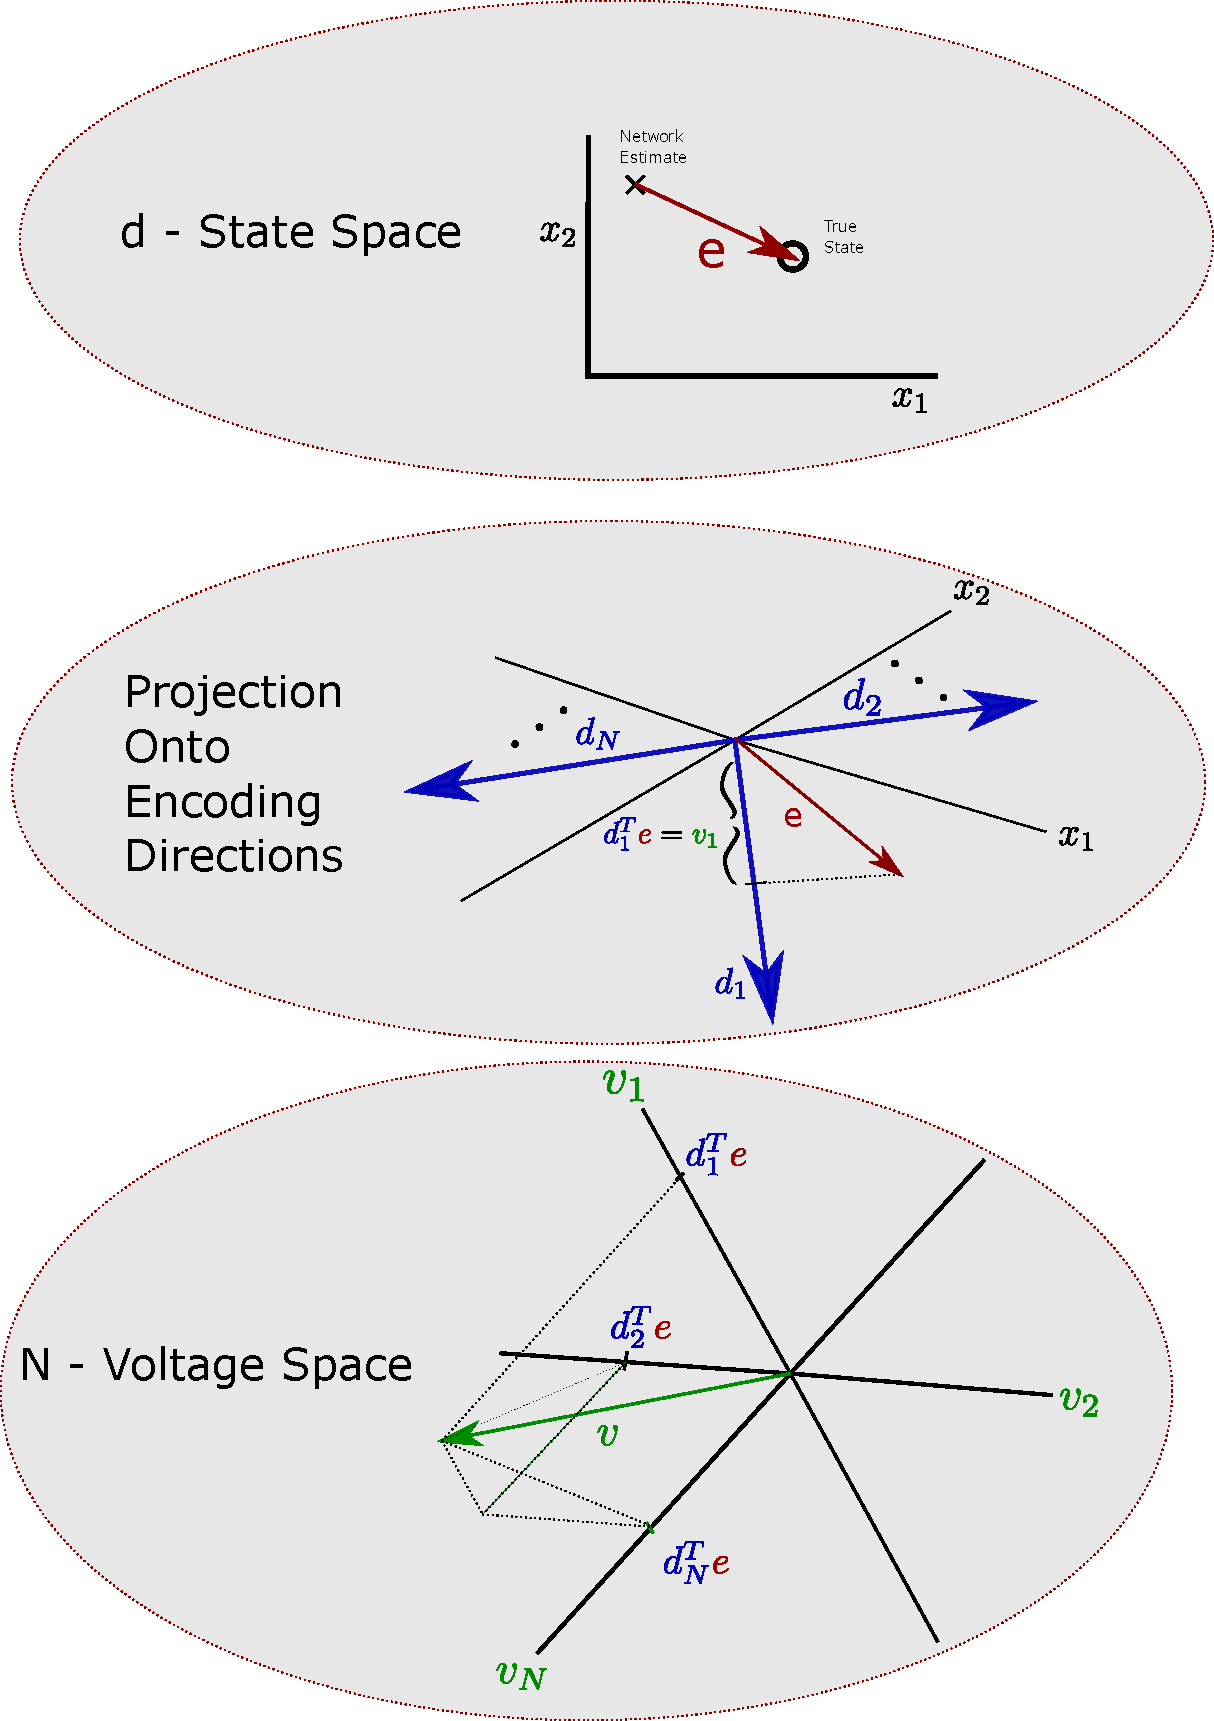
\includegraphics[scale=.703]{figures/pcf_e_v_graphic.pdf}
    \caption{Mapping Between State and Voltage Spaces: \textbf{\textit{Top:}} The estimation error $e$ is computed by comparing the decoded network estimate to the true state of the target dynamical system.  \textbf{\textit{Middle:}} The $e$ is projected onto the encoding directions of the neurons composing the network. The projection of error onto encoding direction $j$ gives the membrane voltage of neuron $j$, $v_j = d_j^T e$. \textbf{\textit{Bottom:}} The voltages form a N-dimensional vector contained in voltage space.}
    \label{fig:derivation:basic_model:pcf_e_v_map}
\end{figure}

\end{enumerate}

\clearpage

\subsection{The Self-Coupled Model is PCF in an Orthonormal Basis}
\begin{enumerate}
\item The self-coupled network is derived from the PCF via a change of bases. Assuming both $D$ and $A$ are full rank, diagonalize each to a common left basis:
\begin{align*}
    A &= \mathcal{U} \Lambda \mathcal{U}^T = \sum_{j=1}^d \Lambda_j \mathcal{U}_j \mathcal{U}_j^T,\\
    \\
    D &= \mathcal{U} \left[S \hspace{2mm} 0 \right]  V^T = \sum_{j=1}^d S_j \mathcal{U}_j  V_j^T,\\
    \\
    D^T &= V \begin{bmatrix} S \\ 0\end{bmatrix} \mathcal{U}^T = \sum_{j=1}^d S_j V_j  \mathcal{U}_j^T, \\
    \\
    D^T D  &= V \begin{bmatrix} S \\ 0\end{bmatrix} \begin{bmatrix} S & 0\end{bmatrix} V^T
     = \sum_{j=1}^d S_j^2 V_j V_j^T , 
\end{align*}
with $\mathcal{U} \in \mathbf{R}^{d \times d}$ and $V \in \mathbf{R}^{N \times N}$, and $S \in \mathbf{R}^{d \times d }$. \\
\\

In the original basis, the state is $x$. In the rotated basis we denote this quantity as $y$. It is the projection of $x$ onto the d-dimensional $\mathcal{U}$ basis:

\begin{align}
\label{eq:definition_rotated_state_space}
y &\overset{\Delta}{=} \mathcal{U}^T x 
%\hat{y} &\overset{\Delta}{=} \mathcal{U}^T \hat{x}.
\end{align}

The rotated target dynamics are thus

\begin{align}
\label{eq:rotated_targed_dynamical_system}
\dot{y} &= \mathcal{U}^T \dot{x} \notag
\\ \notag
\\ \notag
&= 
\Lambda y (\xi)
+
\mathcal{U}^T B c(\xi)
\\ \notag
\\ \notag
&= 
\Lambda y (\xi)
+
\mathcal{U}^T B \mathcal{U} \mathcal{U}^T c(\xi) \notag
\\ \notag
\\ 
&=
\Lambda y (\xi)
+
\beta \tilde{c}(\xi)
\end{align}
where  
$$
\beta \overset{\Delta}{=} \mathcal{U}^T B \mathcal{U},  
$$
and
$$
\tilde{c} \overset{\Delta}{=} \mathcal{U}^T c,
$$
give the projections of $B$ and $c$ respectively.
The network estimate in the rotated basis is 
$$
\hat{y} \overset{\Delta}{=} \mathcal{U}^T \hat{x}.
$$

From equation (\ref{eq:xhat}),
\begin{align*}
\hat{y} &= \mathcal{U}^T \hat{x}
\\ 
\\ 
&=
\mathcal{U}^T D r
\\ 
\\ 
&= 
\begin{bmatrix}
S & 0
\end{bmatrix}
V^T
r
\\
\\
&=
\begin{bmatrix}
S & 0
\end{bmatrix}
\rho
\\
\\
\implies
\dot{\hat{y}}
&= 
\begin{bmatrix}
S & 0
\end{bmatrix}
V^T
\dot{r}
\\
\\
&= 
\begin{bmatrix}
S & 0
\end{bmatrix}
\left( 
-V^T r + V^T o
\right).
\end{align*}

Note that $V^T r$ and $V^T o $ are projections of the N-neuron network's post-synaptic current and spike train respectively onto the rotated basis, denoted by 

\begin{align}
\rho \overset{\Delta}{=} V^T r, 
\label{eq:def_rho}
\\ \notag
\\
\tilde{o} \overset{\Delta}{=} V^T o
\label{eq:def_o_tilde}.
\end{align}

The preceding equality also gives $\hat{y}$ in terms of $\rho$:

\begin{align}
\label{eq:basic:def:y_hat}
\hat{y} = 
\begin{bmatrix}
S & 0
\end{bmatrix}
\rho.
\end{align}

With these definitions, the last equality above also implies

\begin{align}
\label{eq:rho_dot}
\dot{\rho} = -\rho + \tilde{o}.
\end{align}

To finish describing the basic network quantities in terms of the rotated basis, let $\epsilon$ be the error in the rotated basis:
\begin{align}
\label{eq:rotated_error_def}
\epsilon \overset{\Delta}{=} y - \hat{y} \\= \mathcal{U}^T e. \notag
\end{align}

\item Repeat the derivation of equation (\ref{eq:derivation_init}) but with $y$, $\hat{y},$ and $\epsilon$:

\begin{align*}
\dot{\epsilon}
&=
\dot{y} - \dot{\hat{y}}
\\
\\
&= 
\Lambda y + \beta c - 
\begin{bmatrix}
S & 0
\end{bmatrix}
\left(
-\rho + \tilde{o}
\right)
\\
\\
&= 
\Lambda \left(
\epsilon + 
\begin{bmatrix}
S & 0
\end{bmatrix}
\rho
\right)
+ 
\beta tilde{c}
-
\begin{bmatrix}
S & 0
\end{bmatrix}
\left(
-\rho + \tilde{o}
\right)
\\
\\
&= 
\Lambda \epsilon
+
\left( 
\Lambda + I
\right)
\begin{bmatrix}
S & 0
\end{bmatrix}
\rho
+ 
\beta \tilde{c}
-
\begin{bmatrix}
S & 0
\end{bmatrix}
\tilde{o}
\\
\\
\implies
\begin{bmatrix}
S \\ 0
\end{bmatrix}
\dot{\epsilon}
&= 
\begin{bmatrix}
S \\ 0
\end{bmatrix}
\Lambda \epsilon
+
\begin{bmatrix}
S \\ 0
\end{bmatrix}
\left( 
\Lambda + I
\right)
\begin{bmatrix}
S & 0
\end{bmatrix}
\rho
+
\begin{bmatrix}
S \\ 0
\end{bmatrix}
\beta
\tilde{c}
-
\begin{bmatrix}
S \\ 0
\end{bmatrix}
\begin{bmatrix}
S & 0
\end{bmatrix}
\tilde{o}.
\end{align*}

The last equality gives a system of $N$ equations of which only $d$ are nontrivial. A comparison with equation (\ref{eq:derivation_init}) suggests the N-dimensional rotated membrane potential $v$ is best defined as:

\begin{align}
\label{eq:rotated_voltage_def}
v \overset{\Delta}{=} \begin{bmatrix}
S \\ 0
\end{bmatrix} \epsilon \in \mathbf{R}^N.
\end{align}
\\
This mapping is invertible from $v$ to $\epsilon$ if we write  
$$
\epsilon = \begin{bmatrix} S^{-1} & 0 \end{bmatrix}.
$$
This gives a well-defined $d-$vector. whose first $d$ elements are well defined, and the remaining components of $v$ are assumed to be zero. Using a similar abuse for the $\rho$ and $\tilde{o}$ terms, we arrive at the system of $N$ equations describing the network voltage dynamics:
\begin{align}
\label{eq:rotated_voltage_dynamics}
\dot{v}
&= 
\begin{bmatrix}
\Lambda & 0
\\
0 & 0
\end{bmatrix}
v +
\begin{bmatrix}
S \left(\Lambda + I_d \right) S & 0
\\
0 & 0
\end{bmatrix}
  \rho 
  +
\begin{bmatrix}
S \\ 0
\end{bmatrix}  
\beta \tilde{c}
  - 
 \begin{bmatrix}
S^2 & 0
\\
0 & 0
\end{bmatrix}
    \tilde{o}.
\end{align}

To summarize conceptually, there are 4 vector spaces in total: the error space which tracks the dynamical system and the network estimate, the voltage space which tracks the membrane potentials, and the transformed counterparts of each in the $\mathcal{U}-V$ bases. Figure (\ref{fig:four_subspace_relation}) shows the relationships derived between these subspaces.

\begin{figure}[h]
\centering
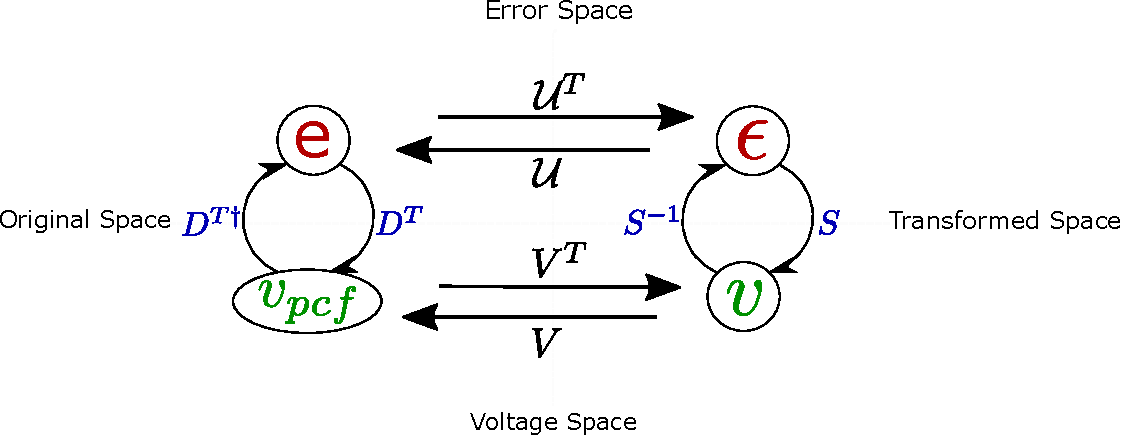
\includegraphics[width=\linewidth]{figures/ev_rotated_classic_graph}
\caption{Depiction of the relationship between original and transformed spaces and their respective error and voltage spaces. An arrow represents left multiplication by the given matrix. The zeros in the full $N \times N$ matrices mapping between $v$ and $\epsilon$ are omitted for clarity.}
\label{fig:four_subspace_relation}
\end{figure}
\end{enumerate}   
\clearpage
   
\subsection{Optimizing Spike-Timing: From PCF to Self-Coupled} 

\begin{enumerate}
\item In PCF, the spike trains $o$ are chosen minimize the network estimation error
\begin{align}
    \mathcal{L}(\xi) =  || x(\xi + d\xi) - \hat{x}(\xi + d\xi) ||^2. 
\end{align}
The network greedily minimizes $\mathcal{L}(\xi)$ an instant $d\xi$ ahead in time. If no spike occurs at time $\xi$, then the objective is given above. If neuron $j$ spikes, the estimate $\hat{x} \leftarrow \hat{x} + d_j$, where $d_j$ is column $j$ of $D$. The objective is now

\begin{align*}
\mathcal{L}_{sp}(\xi) &= ||x - (\hat{x} + d_j)||^2
\\
\\
&= x^T x - 2 \, x^T \hat{x} - 2 x^T d_j + \hat{x}^T \hat{x} + 2 \hat{x}^T d_j + d_j^T d_j
\\
\\
&= x^T x - 2 x^T \hat{x} + \hat{x}^T \hat{x} - 2 d_j^T(x - \hat{x}) + d_j^T d_j
\\
\\
&= ||x - \hat{x}||^2 - 2 d_j^T(x - \hat{x}) + d_j^T d_j
\\
\\
&= 
\mathcal{L}_{ns}(\xi) - 2 d_j^T(x - \hat{x}) + d_j^T d_j,
\end{align*}
where $\mathcal{L}_{ns}(\xi)$ is the objective if no spike occurs. Spiking occurs when the objective decreases or
\begin{align*}
\mathcal{L}_{sp} &< \mathcal{L}_{ns}
\\
\\
\implies
- 2 d_j^T(x - \hat{x}) &+ d_j^T d_j < 0
\\
\\
\implies
d_j^T(x - \hat{x}) >& \frac{||d_j||^2}{2}.
\end{align*}
Since $d_j^T(x-\hat{x}) = d_j^Te$ is already defined as membrane voltage, the right hand side gives neuron $j's$ spike threshold voltage $v_th$,

$$
v_{th}^{pcf} = \frac{1}{2}
\begin{bmatrix}
d_1^T d_1
\\
\vdots
\\
d_N^T d_N
\end{bmatrix}.
$$

\item For the rotated network, note $\mathcal{U}^T$ is an orthonormal matrix by definition. Thus it is norm-preserving:

\begin{align*}
\mathcal{L}_{sp}(\xi) &= ||x - \hat{x}||^2
\\
\\
&= 
||\mathcal{U}^T(x - \hat{x})||^2
\\
\\
&= 
||y - \hat{y}||^2.
\end{align*}

If we define the rotated network objective as 
$$
\tilde{L}(\xi) \overset{\Delta}{=} || y(\xi + d\xi) - \hat{y}(\xi + d\xi)||^2,
$$
it is equal to the original network objective when no spike occurs. However, a spike alters the readout by $\hat{y} \leftarrow \hat{y} + S_l$, where $S_l$ is the $l^{th}$ column of $\begin{bmatrix}
S & 0
\end{bmatrix}$. With the same approach as above, the objective when neuron $l$ spikes is

\begin{align*}
\tilde{L}_{sp} &= \tilde{L}_{ns} + 2 S_l^T\epsilon  + S_l^TS_l
\\
\\
\implies
v_l &> \frac{||S_l||^2}{2}.
\end{align*}

This leads to voltage thresholds

$$
v_{th} = \frac{1}{2}
\begin{bmatrix}
S_1^TS_1
\\
\vdots
\\
S_d^T S_d
\\
0
\\
\vdots
\\
0
\end{bmatrix}. 
$$

\end{enumerate}

\subsection{Consequences of Positive Unit-Area Spikes}
\begin{enumerate}
\item The voltage thresholds are nonnegative, such that neuron $j$ will only spike if 

$$
v_l = S_l^T \epsilon > v_{th} > 0.
$$

The spike form neuron $l$ corrects the network error $\epsilon$ by adding $S_l$ to the estimate $\hat{y}$. The nonnegative voltage implies it is impossible for neuron $l$ to correct antiparallel errors ($-S_l$), since
$$
S_l^T(\epsilon) = S_l^T(-S_l) = - ||S_l||^2 < 0 < v_{th}.
$$

To illustrate consider the space of errors $\epsilon \in \mathbf{R}^d$ which satisfy the voltage threshold of neuron $l$, i.e
$$ 
\epsilon_{sp} = \left\{ \epsilon \in \mathbf{R}^d \, | \, S_l^T \epsilon > v_{th}  \right\}. 
$$

In $\mathbf{R}^2$, $\epsilon_{sp}$ is the half-plane formed by the line normal to $S_l$ shifted $v_{th}$ from the origin along $S_l$ as in figure (\ref{fig:relu_encoding_demo}). This excludes $-S_l$. The optimization thus tells us that neuron $l$ spikes when the projection $S_l^T\epsilon$ exceeds $v_{th}$. 


\begin{figure}
\centering
\includegraphics[scale=.5]{figures/half_plane_relu_demo}
\caption{Sketch of the Encoding space $\epsilon_{sp}$ of neuron $l$ with direction $S_l \in \mathbf{R}^2.$ The radius of the circle is $v_{th}=\frac{||S_l||^2}{2}$. (Vector $S_l$ not drawn to scale).}
\label{fig:relu_encoding_demo}
\end{figure} 

\clearpage


\item Equations (\ref{eq:rotated_voltage_dynamics}) and (\ref{eq:rho_dot}) describe how we implement a network with d neurons that produces an estimate $\hat{y}$ of the given target system. As written, the network can only encode vectors $y$ with strictly nonnegative elements. To see why we return to the optimization procedure performed by the network. 

The network optimizes the objective 

$$
\mathcal{L} = || y - \hat{y}||,
$$

by choosing spike times $\tilde{o}$. The spikes are integrated into a post-synaptic feedback $\rho$. This feedback vector is scaled by $S$ to generate the estimate $\hat{y}$ that minimizes the objective at time $\xi$.  In other words, the network performs the optimization

$$
\underset{\rho \in \mathbf{R}^{d+}}{min} ||y - S \rho ||^2,
$$

where $\mathbf{R}^{d+}$ denotes the real $d-$vectors with nonnegative components. The components must be nonnegative because the spikes $\tilde{o}$ have nonnegative area when integrated, and their dynamics will not decay below zero otherwise. In using a greedy approach with only one spike at a given time step, the network more specifically performs 
$$
\underset{x \in \mathbf{Z}^{d+} \, : \, \sum_j Z_j = 1}{min} ||y - S \left( \rho + x\right) ||^2.
$$

I.e, it must choose one neuron to spike with unit area 1, which adds precisely one column of $S$ to the estimate $\hat{y}$. 

It is easier to analyze the former optimization of $\rho \in \mathbf{R}^{d+}$, and we do so here. Because $ \left\{x \in \mathbf{Z}^{d+} \, : \, \sum_j Z_j = 1 \right\} \subset \mathbf{R}^{d+},$ it is always the case that 
$$
\underset{\rho \in \mathbf{R}^{d+}}{min} ||y - S \rho ||^2
\leq \underset{x \in \mathbf{Z}^{d+} \, : \, \sum_j Z_j = 1}{min} ||y - S \left( \rho + x\right) ||^2,
$$

i.e optimizing over arbitrary $ \rho \in \mathbf{R}^{d+}$ will always give just as low or lower objectives than under the single-greedy spike optimization.

We're interested in the range of vectors representable by the network.  That is the set

$$
X^* = \left\{x \in  \mathbf{R}^{d+} \, \ : \, Sx = y \right\}.
$$


Over this set, the objective function is 0, i.e. 
$$
X^* = \left\{x \in  \mathbf{R}^{d+} \, \ : \, \mathcal{L}=||y-Sx||^2 = 0 \right\}. 
$$

Let $x \in X^*$, and consider its negative $-x$. It follows that 

\begin{align*}
x &= S\rho
\\
\\
\implies -x &= -S \rho
\\
\\
&= S \left(-\rho\right). 
\end{align*}

However if $\rho \in \mathbf{R}^{d+}$, then it is impossible for $-\rho \in \mathbf{R}^{d+}$ to also be true. Thus $-\rho \not\in X^*$ so that $\mathcal{L} > 0$. We conclude that for any vector $\hat{y}$, the network can represent with $\mathcal{L}=0$, there exists a negative vector that the network cannot represent with $\mathcal{L}=0$. This is undesirable as it restricts the set of vectors the network can reconstruct within a given error tolerance. In $\mathbf{R}^2$ for example, network representation where $\mathcal{L} = 0$ is restricted to the first quadrant. This restriction applies equally to the greedy single-spike optimization. 

This issue is unique to the self-coupled network and does not occur in the original PCF network even through its spikes must also have positive unit area. The difference arises when we take the SVD of the decoder matrix.
$$
D = \mathcal{U} \begin{bmatrix} S & 0 \end{bmatrix} V^T.
$$ 

The SVD decomposes $D$ into orthonormal bases $\mathcal{U}$ and $V$ which are mapped to one another by singular values $S$, as in figure (\ref{fig:linear_maps_between_subspaces_D_real}). By rotating into the $\mathcal{U}-V$ bases, we preemptively perform the first and last mappings, leaving only multiplication by a diagonal matrix. This eliminates linearly dependent encoding vectors, keeping only the orthonormal. For example, suppose $x = Dy = \mathcal{U} \begin{bmatrix} S & 0 \end{bmatrix} V^T y$. For an orthonormal basis, $-x$ is obtainable by $\mathcal{U} \begin{bmatrix} S & 0 \end{bmatrix} V^T (-y)$. However the constraint that spikes have positive unit area prevents a vector $\rho=-y$ from being reachable by the network as written. We consider two options to address this below.  




\begin{figure}
\centering
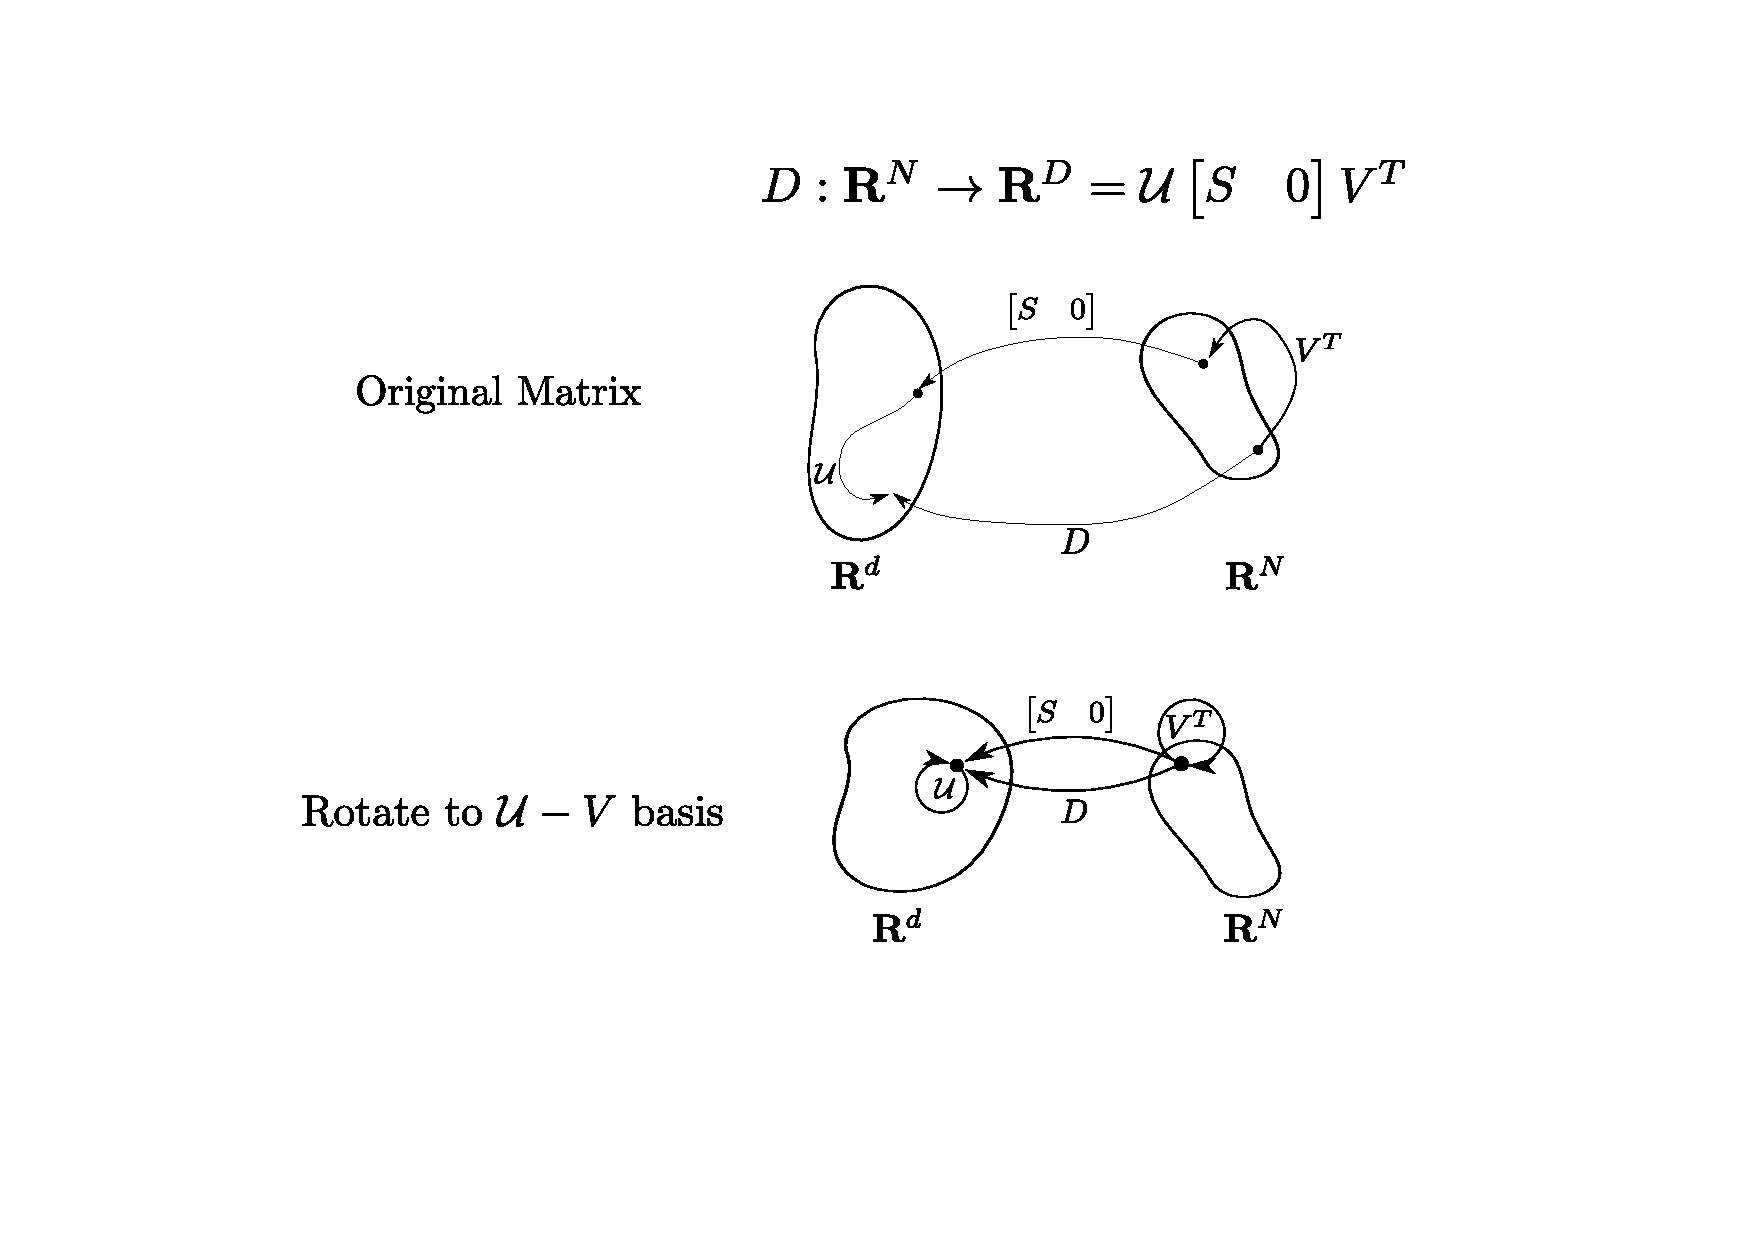
\includegraphics[scale=.6]{figures/linear_map_sequence}
\caption{Visualizing $D$ as a sequence of linear maps between subspaces. \textbf{\textit{Top: }} The matrix $D \in \mathbf{R}^{d \times N}$ is decomposed via SVD into a sequence of 3 linear maps (matrices). The rightmost matrix $V^T \in \mathbf{R}^{N \times N}$ projects a vector  $x$  to give coefficients for the expansion in the basis $V$. The center matrix $\begin{bmatrix} S & 0 \end{bmatrix} \in \mathbf{R}^{d \times N}$ maps vectors from the $V$ basis to a vector in $\mathbf{R}^d$ by scaling and truncation. The leftmost matrix $\mathcal{U} \in \mathbf{R}^{d \times d}$ gives the resultant vector $D x \in \mathbf{R}^d$ by using the scaled vector $\begin{bmatrix} S & 0 \end{bmatrix} V^T$  as coefficients for a basis expansion in $\mathcal{U}$. \textbf{\textit{Bottom:}} We rotate the basis for vectors in $\mathbf{R}^N$ and $\mathbf{R}^d$ to the $\mathcal{U}$ and $V$ bases respectively. This negates the need of $D$ to preemptively project and afterward rotate a vector, leaving only scaling by a diagonal matrix. The mapping $D$ performs on a vector $y$ simplifies to multiplication by a diagonal matrix $S$ of $y$'s first $d$ components. 
}
\label{fig:linear_maps_between_subspaces_D_real}
\end{figure}

\clearpage

\item For the network decoder to fully span the state space of interest, it must have anti-parallel encoding directions even in the rotated orthonormal basis. To do so we augment the rotated bases by adding an antiparallel set so they are no longer orthonormal. We consider two methods of adding antiparallel bases: 

\textbf{\textit{Method A: Separate Antiparallel Networks}} One solution is to form a separate network of $d$ neurons whose encoding directions are the antiparallel set $-\mathcal{U}$. That is, we form an identical network except the decode matrix is
$$ -D = -\mathcal{U} \begin{bmatrix} S & 0 \end{bmatrix} V^T.$$

We then add the output of the two networks to recover the encoded state. 


We divide the error into its positive and negative components and encode each in a separate network. Let
$$
\epsilon^{+} = \epsilon \geq 0,
$$

be the nonnegative component of $\epsilon$. Note that the original estimate, $e$ may contain negative or positive components, but the projection $\epsilon^{+}$ does not.  Similarly define the negative error by 

$$
\epsilon^{-} = -\epsilon < 0.
$$

Note
$$
\epsilon^{-} \neq -\epsilon^+. 
$$
Rather, 
$$
\epsilon = \epsilon^{+} - \epsilon^{-}.
$$

The relationship between $\epsilon^+$ and $\epsilon^-$ resembles two orthogonal subspaces. The preceding relation is analogous to a direct sum. 


Let
$$
v^{+} = S^T \epsilon^+, 
$$
be the voltage induced by projecting $\epsilon^+$ onto the orthonormal bases given by $D = \mathcal{U} \begin{bmatrix} S & 0 \end{bmatrix} V^T$,

and 
$$
v^{-} = S^T \epsilon^-
$$

be the respective projection onto the antiparallel orthonormal bases, $D = \mathcal{U} \begin{bmatrix} -S & 0 \end{bmatrix} V^T$.

Note that
$$
v^{-} \neq -v^+. 
$$
Rather, 
$$
v= v^{+} - v^{-}, 
$$

where $v$ is the voltage of an idealized neuron capable of positive and negative area spikes. Note that both $v_j^+$ and $v_j^-$ are bounded by thresholds $v_{th} = \frac{||S_j||^2}{2}$, so that the idealized neuron is always within the voltage range $v \in \left[ -v_{th}, v_{th} \right]$. This is equivalent to asserting the error along each encoding direction $S_j$ is contained within the polytope $S_j^T \epsilon \leq \frac{||S_j||^2}{2}$. 

Let $\rho^+$ and $\tilde{o}^+$ be the slow synaptic feedback and spike trains of the positive neurons, with $\rho^-$ and $\tilde{o}^-$ defined similarly for the negative neurons. Finally split $\tilde{c} = \tilde{c}^+ - \tilde{c}^-$ into positive and negative components as with $\epsilon$.  

 We now have two $d-$dimensional systems of equations.  
\begin{align*}
\dot{v}^{+}
&= 
\begin{bmatrix}
\Lambda & 0
\\
0 & 0
\end{bmatrix}
v^+ +
\begin{bmatrix}
S \left(\Lambda + I_d \right) S & 0
\\
0 & 0
\end{bmatrix}
  \rho^+
  +
\begin{bmatrix}
S \\ 0
\end{bmatrix}  
\beta \tilde{c}^+
  - 
 \begin{bmatrix}
S^2 & 0
\\
0 & 0
\end{bmatrix}
    \tilde{o}^+,
    \\
    \\
    \dot{v}^{-}
&= 
\begin{bmatrix}
\Lambda & 0
\\
0 & 0
\end{bmatrix}
v^- +
\begin{bmatrix}
S \left(\Lambda + I_d \right) S & 0
\\
0 & 0
\end{bmatrix}
  \rho^-
  +
\begin{bmatrix}
S \\ 0
\end{bmatrix}  
\beta \tilde{c}^-
  - 
 \begin{bmatrix}
S^2 & 0
\\
0 & 0
\end{bmatrix}
    \tilde{o}^-.
\end{align*}


These equations each produce estimates 
$$
\hat{y}^+ = S \rho^+,
$$

$$
\hat{y}^- = S \rho^-,
$$

which give the network estimate

$$
\hat{y} = \hat{y}^+ - \hat{y}^-.
$$



Writing the above as a single network, assume $N = 2d$ so we need not fill with zeros:

$$
\begin{bmatrix}\dot{v}^+\\ \dot{v}^-\end{bmatrix} = \begin{bmatrix}
\Lambda & 0
\\
0 & \Lambda 
\end{bmatrix}
\begin{bmatrix} v^+ \\ v^- \end{bmatrix}
 +
\begin{bmatrix}
S \left(\Lambda + I_{d} \right) S & 0 
\\
0 & S \left(\Lambda + I_{d} \right) S 
\end{bmatrix}
\begin{bmatrix}
  \rho^+
  \\
  \rho^-
\end{bmatrix}
  +
\begin{bmatrix}
S & 0 \\ 0 & S
\end{bmatrix}  
\beta 
\begin{bmatrix}
\tilde{c}^+
\\
\tilde{c}^-
\end{bmatrix}
  - 
 \begin{bmatrix}
S^2 & 0
\\
0 & S^2
\end{bmatrix}
\begin{bmatrix}
    \tilde{o}^+
    \\
    \tilde{o}^-
\end{bmatrix}
.
$$

We simplify this by writing 

$$
   \dot{v}
= 
\Lambda 
v +
S \left(\Lambda + I_{2d} \right) S 
  \rho
  +
S 
\beta \tilde{c}
  - 
S^2 
    \tilde{o}, 
$$


where we have made the following substitutions: 

\begin{align*}
	v &\leftarrow \begin{bmatrix}
	v^+ \\ v^-
	\end{bmatrix} 
	    \in \mathbf{R}^{2 d},
	\\
	\\
	\Lambda &\leftarrow
    \begin{bmatrix}
    \Lambda & 0 \\ 0 & \Lambda
    \end{bmatrix}
    \in \mathbf{R}^{2 d \times 2 d},
    \\
    \\
    S &\leftarrow
    \begin{bmatrix}
    S & 0 \\ 0 & S
    \end{bmatrix}
   \in \mathbf{R}^{2 d \times 2 d},\\
    \\
    \rho &\leftarrow 
    \begin{bmatrix}
    \rho^+ \\ \rho^-
    \end{bmatrix} \in \mathbf{R}^{2d},
    \\
    \\
    \tilde{o} &\leftarrow 
    \begin{bmatrix}
    \tilde{o}^+ \\ \tilde{o}^-
    \end{bmatrix} \in \mathbf{R}^{2d},
    \\
    \\
    \beta &\leftarrow 
    \begin{bmatrix}
    \beta & 0 \\ 0 & \beta
    \end{bmatrix}
    \in \mathbf{R}^{2d \times 2d},
    \\
    \\
    \tilde{c} & \leftarrow 
    \begin{bmatrix}
    \tilde{c}^+ \\ \tilde{c}^-
    \end{bmatrix} \in \mathbf{R}^{2d},
    \\
    \\
    v_{th} &\leftarrow 
    \begin{bmatrix}
    v_{th} \\ v_{th}
    \end{bmatrix} \in \mathbf{R}^{2d}.
\end{align*}

To decode from the network to the $d-$dimensional estimate, we multiply by $ \begin{bmatrix}
\mathcal{U} & -\mathcal{U}
\end{bmatrix} \in \mathbf{R}^{d \times 2d},$ i.e 
$$
\hat{y} = \hat{y}^+ - \hat{y}^- = \begin{bmatrix}
\mathcal{U} & -\mathcal{U}
\end{bmatrix} \rho.
$$
\clearpage



This approach suggests a balance between excitatory and inhibitory neurons when coding an oscillatory signal that inhabits the full $d-$dimensional state space. To illustrate, consider a 2 neuron network as in figure (\ref{fig:ei_balance_demo}). An input $\tilde{c}(\xi) = sin(\omega \xi)$ drives the neurons which encode $v^+$ and $v^-$ respectively. A readout neuron performs leaky integration of the spike trains from the two driven neurons. Consider how a received spike changes the voltage of the readout neuron. A spike from one neuron will increase the readout neuron's membrane potential (excitatory input), while a spike from the other neuron must symmetrically decrease the readout neuron's potential (inhibitory input). In this case, we observe equal levels of excitatory (and inhibitory input from the two neurons, suggesting a tight balance. Note also this ensures consistency with Dale's law, which states that a neuron cannot both excite and inhibit other neurons. 

\begin{figure}
\centering

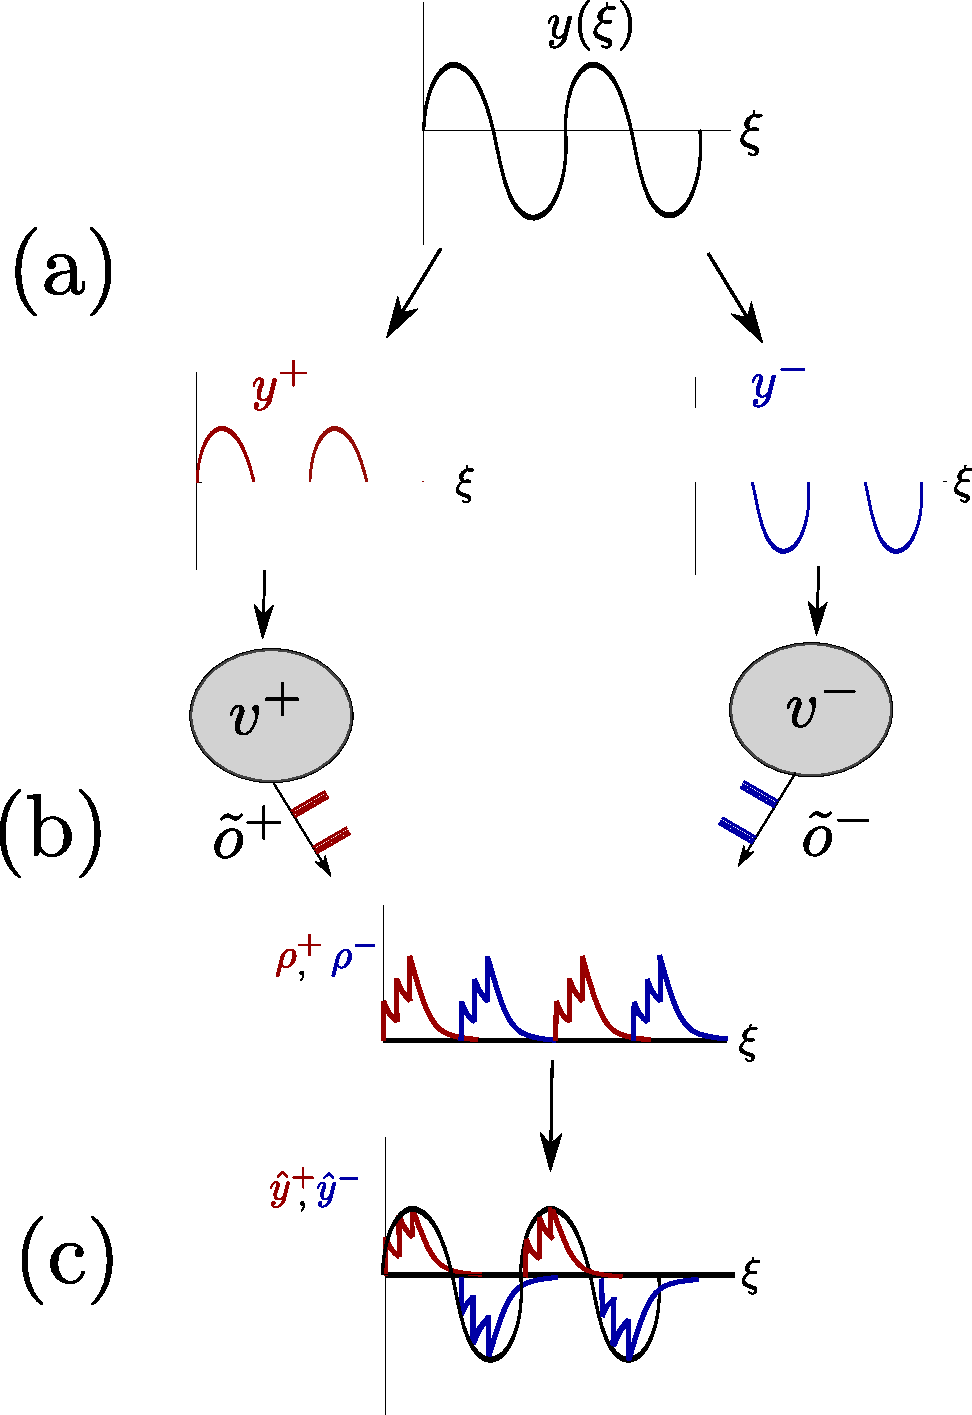
\includegraphics[width=\linewidth, height=19cm]{figures/demo_balance_ei}
\caption{Balance Between Excitatory and Inhibitory Activity for Oscilllatory Input. \textbf{\textit{(a):}} A sinusoidal input $y$ is divided into its positive (excitatory) and negative (inhibitory) components.\textbf{\textit{(b):}} Each neuron encodes its respective input by spiking to produce a nonnegative filtered spike train $\rho$. \textbf{\textit{(c):}} } The network estimate is the sum of activity from excitatory and inhibitory filtered spike trains. For oscillatory input, both neurons must spike in equal amounts so that the amplitude of oscillation remains bounded. 
\label{fig:ei_balance_demo}
\end{figure}


Note also that the fast coupling matrix preceding $\tilde{o}$ is diagonal. This implies that when a neuron $j$ spikes, its antiparallel neuron is unchanged. In the PCF, a neuron spike resets its threshold to $-v_{th}$, but likewise sets a neuron antiparallel to it to $v_{th}$. Next, the antiparallel neuron spikes and likewise resets the neuron. This cycle repeats itself causing the network estimate to oscillate uncontrollably in a catastrophic network failure termed "ping-ponging". The PCF addresses this through regularization terms applied to the network objective $\mathcal{L}$ and added noise,  (Boerlin 2013) both of which are unnecessary in this case. 
\end{enumerate}

\clearpage

\textbf{\textit{Method B: Fast-Coupling Between Antiparallel Neurons}} The other method we consider maintains the fast-coupling relationship between a neuron and its opposite as described in PCF. Fast-coupling implies that when a neuron $i$ with encoding direction $d_i$ spikes, neuron $j$'s voltage changes by $-d_j^T d_i$. This is visible in the spiking ($D^TDo$) term in PCF's voltage equation (\ref{eq:derivation_init}). If $d_j = -d_i$, then a spike in $d_j$ decreases $j$'s voltage by $||d_j||^2$, while simultaneously increasing neuron $i$'s voltage by the same. 

\begin{enumerate}



\item  Previously we used a subset of $d$ neurons from the decoder matrix, 
$$
D = \mathcal{U} \begin{bmatrix}
S & 0
\end{bmatrix}
V^T \in \mathbf{R}^{d \times N}.
$$

In adding $d$ antiparallel neurons, we assume $N \geq 2d$ and instead use $2d$ neurons, i.e. we write
$$
D = \begin{bmatrix}
\mathcal{U} & -\mathcal{U}
\end{bmatrix}^T \begin{bmatrix}
S & 0 & 0
\\
0 & S & 0
\end{bmatrix}
V^T \in \mathbf{R}^{d \times N}.
$$

The first and second $d$ neurons have encoding directions $\mathcal{U}$ and $-\mathcal{U}$ respectively. Before the first $d$ right eigenvectors $V_j$ were scaled by $\sigma_j$ and mapped to $\mathcal{U}_j$, with the remaining $V_j$ mapped to $0$. In adding $d$ antiparallel vectors, we scale an additional $d$ right eigenvectors $V_{j+d}$ by $\sigma_j$ and map them to $-\mathcal{U}_j$. 


Note that our change of basis should be invertible by its transpose and norm-preserving. Before, this meant
$$
\mathcal{U} \mathcal{U}^T x = x.
$$

Now we require
$$
\begin{bmatrix}
\mathcal{U} & -\mathcal{U}
\end{bmatrix} \begin{bmatrix}
\mathcal{U} & -\mathcal{U}
\end{bmatrix}^T x = x,
$$

but 

\begin{align*}
\begin{bmatrix}
\mathcal{U} & -\mathcal{U}
\end{bmatrix} \begin{bmatrix}
\mathcal{U} & -\mathcal{U}
\end{bmatrix}^T x
&=
\begin{bmatrix}
\mathcal{U} & -\mathcal{U}
\end{bmatrix}
\begin{bmatrix}
\mathcal{U}^T x \\ -\mathcal{U}^T x
\end{bmatrix}
\\
\\
&=
\mathcal{U} \mathcal{U}^T x + \mathcal{U}\mathcal{U}^T x
\\
\\
&=
2x.
\end{align*}

So our desired basis is actually
$$
\frac{1}{\sqrt{2}} 
\begin{bmatrix}
\mathcal{U} & -\mathcal{U}
\end{bmatrix}.
$$

Therefore we write the decode matrix instead as 
$$
D = \frac{1}{\sqrt{2}}\begin{bmatrix}
\mathcal{U} & -\mathcal{U}
\end{bmatrix}^T \begin{bmatrix}
S & 0 & 0
\\
0 & S & 0
\end{bmatrix}
V^T \in \mathbf{R}^{d \times N}.
$$


In terms of the basis $\frac{1}{\sqrt{2}} \begin{bmatrix} \mathcal{U} & -\mathcal{U}\end{bmatrix},$ the state becomes

$$
y = \mathcal{U}^T x \leftarrow \frac{1}{\sqrt{2}}\begin{bmatrix}
\mathcal{U} & -\mathcal{U}
\end{bmatrix}^T x = \frac{1}{\sqrt{2}} \begin{bmatrix}
y\\-y
\end{bmatrix} \in \mathbf{R}^{2d}.
$$


This gives the dynamical system
\begin{align*}
\dot{y} &= \frac{1}{\sqrt{2}} \begin{bmatrix}
\mathcal{U} & -\mathcal{U}
\end{bmatrix}^T \dot{x}
\\
\\
&=
\frac{1}{\sqrt{2}} \begin{bmatrix}
\mathcal{U} & -\mathcal{U}
\end{bmatrix}^T \mathcal{U} \Lambda \mathcal{U}^T x + \frac{1}{\sqrt{2}}  \begin{bmatrix}
\mathcal{U} & -\mathcal{U}
\end{bmatrix}^T B c.
\end{align*}

The first term becomes
\begin{align*}
\frac{1}{\sqrt{2}} \begin{bmatrix}
\mathcal{U} & -\mathcal{U}
\end{bmatrix}^T \mathcal{U} \Lambda \mathcal{U}^T x
&=
\frac{1}{\sqrt{2}} \begin{bmatrix}
I \\ -I
\end{bmatrix}
\Lambda \mathcal{U}^T x
\\
\\
&=
\frac{1}{\sqrt{2}} \begin{bmatrix}
\Lambda \mathcal{U}^T
\\
-\Lambda \mathcal{U}^T 
\end{bmatrix} x
\\
\\
&=
\frac{1}{\sqrt{2}}
\begin{bmatrix}
\Lambda & 0
\\
0 & \Lambda
\end{bmatrix}
\begin{bmatrix}
\mathcal{U} & -\mathcal{U}
\end{bmatrix}^T x
\\
\\
&=
\frac{1}{\sqrt{2}}
\begin{bmatrix}
\Lambda & 0 
\\
0 & \Lambda
\end{bmatrix}
\begin{bmatrix} y \\ -y \end{bmatrix} \in \mathbf{R}^{2d}.
\end{align*}

The latter input term which previously formed the drive term $\beta \tilde{c}$ becomes

$$
\tilde{c} = \mathcal{U}^T c \leftarrow \frac{1}{\sqrt{2}}\begin{bmatrix}
\mathcal{U} & -\mathcal{U} 
\end{bmatrix}^T \tilde{c} = 
\frac{1}{\sqrt{2}}\begin{bmatrix}
\tilde{c} \\ \tilde{c}
\end{bmatrix} \in \mathbf{R}^{2d},
$$

$$
\beta = \mathcal{U}^T B \mathcal{U} \leftarrow
\frac{1}{2}\begin{bmatrix}
\mathcal{U} & -\mathcal{U} 
\end{bmatrix}^T
B
\begin{bmatrix}
\mathcal{U} & -\mathcal{U} 
\end{bmatrix}
=
\frac{1}{2}\begin{bmatrix}
\beta & -\beta
\\
-\beta & \beta
\end{bmatrix} \in \mathbf{R}^{2d \times 2d}.
$$

The rotated dynamical system is thus
$$
\dot{y} = \frac{1}{\sqrt{2}} \begin{bmatrix}
\Lambda & 0
\\
0 & \Lambda
\end{bmatrix}
\begin{bmatrix}
y\\-y
\end{bmatrix}
+ 
\frac{1}{2\sqrt{2}}
\begin{bmatrix}
\beta & -\beta
\\
-\beta & \beta
\end{bmatrix}
\begin{bmatrix}
\tilde{c}
\\
\tilde{c}
\end{bmatrix}.
$$




\item The network estimation 
$$
\hat{y}  = \mathcal{U}^T \hat{x} = \mathcal{U}^T \begin{bmatrix}
S & 0
\end{bmatrix} 
V^T r
$$
is now

\begin{align*}
\hat{y} = \frac{1}{\sqrt{2}}\begin{bmatrix}
\mathcal{U} & -\mathcal{U}
\end{bmatrix}^T
\hat{x}
&=
\frac{1}{2}\begin{bmatrix}
\mathcal{U} & -\mathcal{U}
\end{bmatrix} ^T \begin{bmatrix}
\mathcal{U} & -\mathcal{U}
\end{bmatrix} \begin{bmatrix}
S & 0 & 0
\\
0 & S & 0
\end{bmatrix}
V^T r
\\
\\
&=
\frac{1}{2}\begin{bmatrix}
S & -S & 0
\\
-S & S & 0
\end{bmatrix}
\rho \in \mathbf{R}^{2d}.
\end{align*}

The error goes from 
$$
\epsilon = y - \hat{y} \in \mathbf{R}^d
$$

to

$$
\epsilon = \frac{1}{\sqrt{2}}\begin{bmatrix}
y \\ - y
\end{bmatrix}
-
\frac{1}{2}\begin{bmatrix}
S & -S & 0
\\
-S & S & 0
\end{bmatrix}
\rho \in \mathbf{R}^{2d}.
$$

We rederive the error dynamics 
\begin{align*}
\dot{\epsilon} &= \dot{y} - \dot{\hat{y}}
\\
\\
&=
\frac{1}{\sqrt{2}} \begin{bmatrix}
\Lambda & 0
\\
0 & \Lambda
\end{bmatrix}
\begin{bmatrix}
y\\-y
\end{bmatrix}
+ 
\frac{1}{2\sqrt{2}}
\begin{bmatrix}
\beta & -\beta
\\
-\beta & \beta
\end{bmatrix}
\begin{bmatrix}
\tilde{c}
\\
\tilde{c}
\end{bmatrix} -
\frac{1}{2}\begin{bmatrix}
S & -S & 0
\\
-S & S & 0
\end{bmatrix} \left( -\rho + \tilde{o}\right)
\\
\\
&= 
\begin{bmatrix}
\Lambda & 0
\\
0 & \Lambda
\end{bmatrix}
\left(
\epsilon + \hat{y}
\right)
+ 
\frac{1}{2\sqrt{2}}
\begin{bmatrix}
\beta & -\beta
\\
-\beta & \beta
\end{bmatrix}
\begin{bmatrix}
\tilde{c}
\\
\tilde{c}
\end{bmatrix} -
\frac{1}{2}\begin{bmatrix}
S & -S & 0
\\
-S & S & 0
\end{bmatrix} \left( -\rho + \tilde{o}\right)
\\
\\
&=
\begin{bmatrix}
\Lambda & 0
\\
0 & \Lambda
\end{bmatrix}
\epsilon
+ 
\frac{1}{2}
\left(
\begin{bmatrix}
\Lambda & 0
\\
0 & \Lambda
\end{bmatrix}
+ I
\right)
\begin{bmatrix}
S & -S & 0
\\
-S & S & 0
\end{bmatrix} \rho
+
\frac{1}{2\sqrt{2}}
\begin{bmatrix}
\beta & -\beta
\\
-\beta & \beta
\end{bmatrix}
\begin{bmatrix}
\tilde{c}
\\
\tilde{c}
\end{bmatrix}
-
\frac{1}{2}\begin{bmatrix}
S & -S & 0
\\
-S & S & 0
\end{bmatrix} \tilde{o}.
\end{align*}

\item We previously obtained voltage by optimizing the objective

$$
\mathcal{L} = ||y - \hat{y}||^2. 
$$

When neuron $j$ spikes before, we added the $j^{th}$ column of the decoding matrix which mapped $\rho \to \hat{y}$. This was the matrix $\begin{bmatrix}S & 0 \end{bmatrix}$. It is now 
$$
\frac{1}{2} \begin{bmatrix}
S & -S & 0 
\\
-S & S & 0
\end{bmatrix}.
$$

When neuron $j$ spikes we thus add $\frac{1}{2}\begin{bmatrix} S_j & -S_j \end{bmatrix}$ to the network estimate. I.e.

\begin{align*}
\mathcal{L}_{spike} &= || 
\frac{1}{\sqrt{2}}
\begin{bmatrix}
y \\-y
\end{bmatrix}
-
\frac{1}{2}
\begin{bmatrix}
S & - S & 0 
\\
-S & S & 0
\end{bmatrix}\rho
-
\frac{1}{2}
\begin{bmatrix}
S_j \\ -S_j
\end{bmatrix}
||^2
\\
\\
&=
\frac{1}{2}
\begin{bmatrix}
y \\-y
\end{bmatrix}^T \begin{bmatrix}
y \\-y
\end{bmatrix}
\\
 &- \frac{1}{\sqrt{2}}
 \begin{bmatrix}
y \\-y
\end{bmatrix}^T \begin{bmatrix}
S & - S & 0 
\\
\\
-S & S & 0
\end{bmatrix}\rho
\\
\\
&+ 
\frac{1}{4}
\left(\begin{bmatrix}
S & - S & 0 
\\
\\
-S & S & 0
\end{bmatrix}\rho\right)^T \begin{bmatrix}
S & - S & 0 
\\
\\
-S & S & 0
\end{bmatrix}\rho
\\
\\
&- 
2\, \begin{bmatrix}
S_j \\ -S_j
\end{bmatrix}^T \left(\frac{1}{\sqrt{2}}
\begin{bmatrix}
y \\-y
\end{bmatrix}
-
\frac{1}{2}
\begin{bmatrix}
S & - S & 0 
\\
-S & S & 0
\end{bmatrix}\rho \right)
\\
\\
&+
\frac{1}{4}
\begin{bmatrix}
S_j \\ -S_j
\end{bmatrix}^T\begin{bmatrix}
S_j \\ -S_j
\end{bmatrix}
\\
\\
&=
\mathcal{L}_{ns} - \begin{bmatrix}
S_j \\ -S_j
\end{bmatrix}^T \left( \frac{1}{\sqrt{2}}
\begin{bmatrix}
y \\-y
\end{bmatrix}
-
\frac{1}{2}
\begin{bmatrix}
S & - S & 0 
\\
-S & S & 0
\end{bmatrix}\rho \right)
+
\frac{1}{4}
\begin{bmatrix}
S_j \\ -S_j
\end{bmatrix}^T\begin{bmatrix}
S_j \\ -S_j
\end{bmatrix}.
\end{align*}

The spiking rule becomes

\begin{align*}
- \begin{bmatrix}
S_j \\ -S_j
\end{bmatrix}^T \left( \frac{1}{\sqrt{2}}
\begin{bmatrix}
y \\-y
\end{bmatrix}
-
\frac{1}{2}
\begin{bmatrix}
S & - S & 0 
\\
-S & S & 0
\end{bmatrix}\rho \right)
+
\frac{1}{4}
\begin{bmatrix}
S_j \\ -S_j
\end{bmatrix}^T\begin{bmatrix}
S_j \\ -S_j
\end{bmatrix} &< 0
\\
\\
&\implies
-\begin{bmatrix}
S_j \\
-S_j
\end{bmatrix}^T
\begin{bmatrix}
\epsilon 
\\
-\epsilon
\end{bmatrix} + \frac{1}{2}||S_j||^2 &< 0
\\
\\
&\implies
-2 \, S_j^T \epsilon < ||S_j||^2
\\
\\
&\implies
S_j^T \epsilon > \frac{||S_j||^2}{2}.
\end{align*}

Thus the voltage definition for neuron $j$ $v_j = S_j^T \epsilon$ remains unchanged. The matrix expression is changed however. Applying the decode matrix to the error $\epsilon$ gives

$$
v = 
\frac{1}{2}
\begin{bmatrix}
S & - S & 0
\\
-S & S & 0
\end{bmatrix}^T \epsilon.
$$

From the error dynamics, we arrive at the voltage dynamics using the above relation:

\begin{align*}
\dot{v} &= 
\frac{1}{2}
\begin{bmatrix}
S & - S & 0
\\
-S & S & 0
\end{bmatrix}^T
\begin{bmatrix}
\Lambda & 0
\\
0 & \Lambda
\end{bmatrix}
\epsilon
\\
\\
&+ 
\frac{1}{4}
\begin{bmatrix}
S & - S & 0
\\
-S & S & 0
\end{bmatrix}^T
\left(
\begin{bmatrix}
\Lambda & 0
\\
0 & \Lambda
\end{bmatrix}
+ I
\right)
\begin{bmatrix}
S & -S & 0
\\
-S & S & 0
\end{bmatrix} \rho
\\
\\
&+
\frac{1}{4\sqrt{2}}
\begin{bmatrix}
S & - S & 0
\\
-S & S & 0
\end{bmatrix}^T
\begin{bmatrix}
\beta & -\beta
\\
-\beta & \beta
\end{bmatrix}
\begin{bmatrix}
\tilde{c}
\\
\tilde{c}
\end{bmatrix}
\\
\\
&-
\frac{1}{4}
\begin{bmatrix}
S & - S & 0
\\
-S & S & 0
\end{bmatrix}^T
\begin{bmatrix}
S & -S & 0
\\
-S & S & 0
\end{bmatrix} \tilde{o}
\\
\\
\end{align*}

This gives
\begin{align*}
\dot{v}
&=
\begin{bmatrix}
\Lambda & 0
\\
0 & \Lambda
\end{bmatrix} v 
\\
\\
&+ 
\frac{1}{4}
\begin{bmatrix}
S & - S & 0
\\
-S & S & 0
\end{bmatrix}^T
\left(
\begin{bmatrix}
\Lambda & 0
\\
0 & \Lambda
\end{bmatrix}
+ I
\right)
\begin{bmatrix}
S & -S & 0
\\
-S & S & 0
\end{bmatrix} \rho
\\
\\
&+
\frac{1}{4\sqrt{2}}
\begin{bmatrix}
S & - S & 0
\\
-S & S & 0
\end{bmatrix}^T
\begin{bmatrix}
\beta & -\beta
\\
-\beta & \beta
\end{bmatrix}
\begin{bmatrix}
\tilde{c}
\\
\tilde{c}
\end{bmatrix}
\\
\\
&-
\frac{1}{2}
\begin{bmatrix}
S^2 & -S^2 & 0 
\\
-S^2 & S^2 & 0
\\
0 & 0 & 0
\end{bmatrix} \tilde{o}.
\end{align*}

Recall that $S \in \mathbf{R}^{d x d}$ is a diagonal matrix with entries $\sigma_j$. As desired, the spike matrix applied to $\tilde{o}$ implements fast coupling between antiparallel neurons.  When neuron $j$ spikes, it is decreased by $||\sigma_j||^2$, while its antiparallel counterpart $S_{j + d}$ is increased by $\sigma_j^2$. 

\item To facilitate comparison between the self-coupled network and original PCF model, we will use this method (B) hereafter. Method A is a viable alternative, however it is fundamentally different than the original PCF model because antiparallel neurons do not interact in contrast with PCF and method B.  We investigate method A later. 
\end{enumerate}


\clearpage

\subsection{Simulation of Basic Equations}
Here we simulate the above equations (\ref{eq:rotated_voltage_dynamics}) and (\ref{eq:rho_dot}) with the $N = 2d$ neurons. The parameters are
\begin{align}
\label{eq:sim_I_params}
A
&=
\ -\begin{bmatrix}  
1 & 0 \\
0 & 1
\end{bmatrix} = \mathcal{U} \Lambda \mathcal{U}^T \notag,
\\
\notag
\\
B
&=
\begin{bmatrix}  
1 & 0 \\
0 & 1
\end{bmatrix}, \notag 
\\
\notag 
\\
c(\xi) 
&=
\begin{bmatrix} 
cos(\frac{\pi}{4} \xi)\\
sin(\frac{\pi}{4} \xi)
\end{bmatrix} 
\\
\notag
\\
D
&=
\mathcal{U} 
\begin{bmatrix}
S & 0
\end{bmatrix}
V^T
=
\mathcal{U} 
\begin{bmatrix}
.1 \, I_d & 0
\end{bmatrix}
I_N \notag,
\\
\notag 
\\
d\xi 
&= 
10^{-6}, \notag 
\\
\notag 
\\
N 
&= 
4,\notag 
\\
\notag 
\\
x(0) 
&= 
\begin{bmatrix} \frac{1}{2} & \frac{1}{2} \end{bmatrix}.\notag 
\end{align}

\begin{figure}
    \centering
    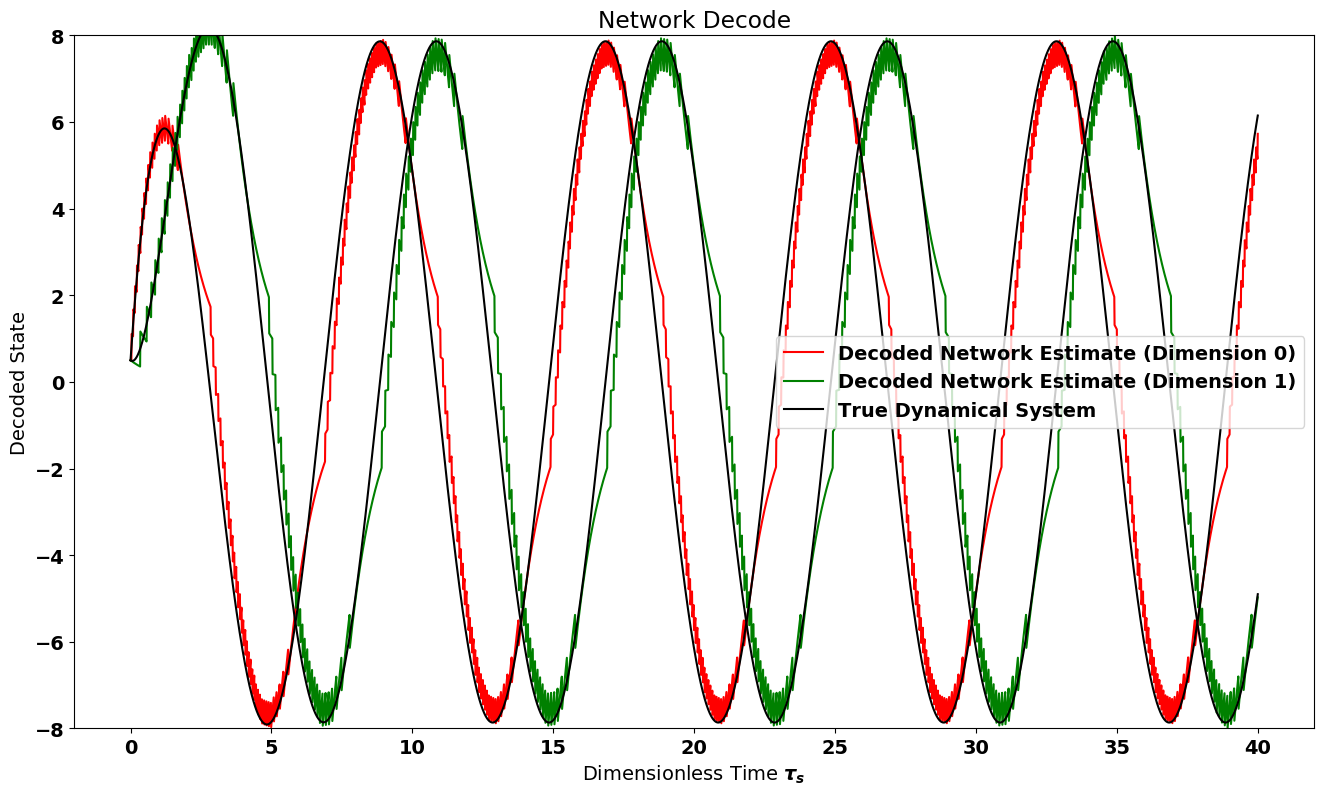
\includegraphics[width=.75\linewidth]{figures/network_decode.png}

    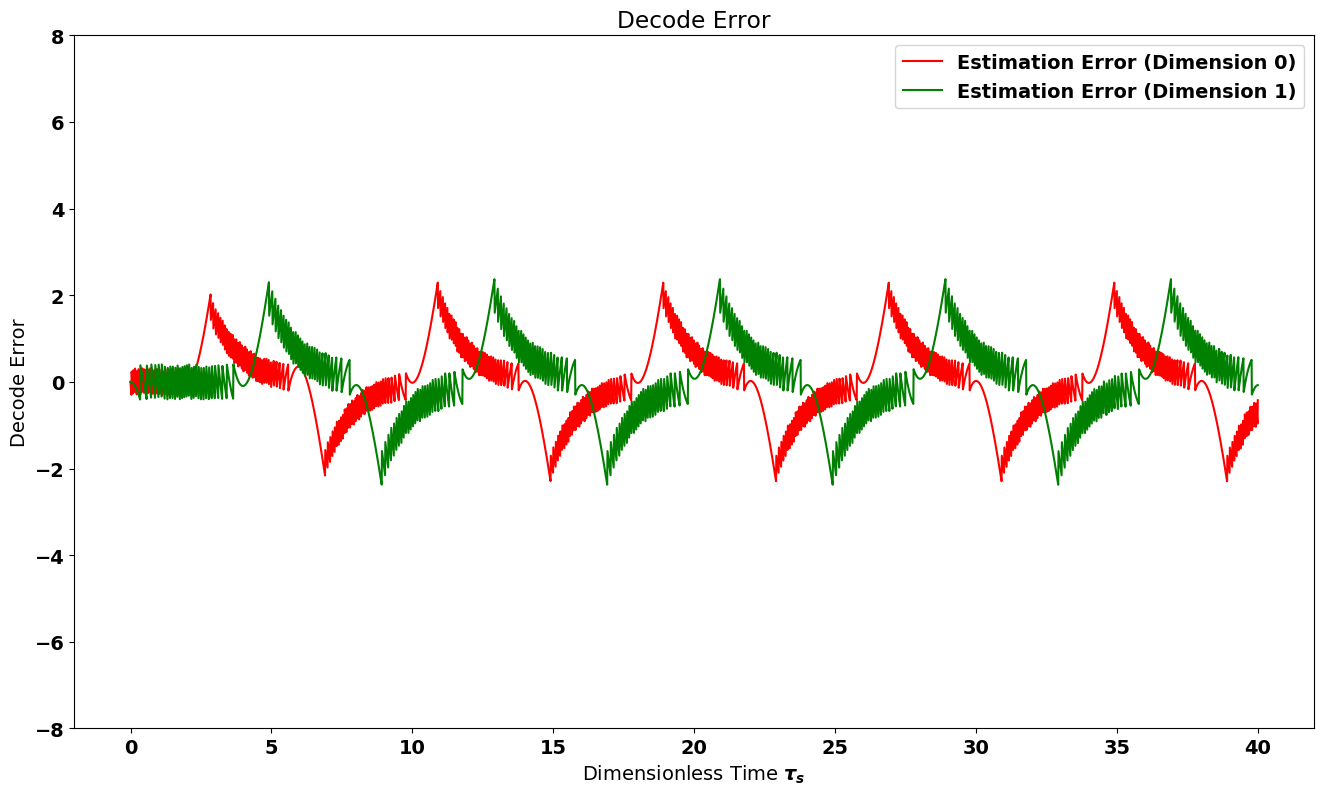
\includegraphics[width=.75\linewidth]{figures/decode_error.png}

    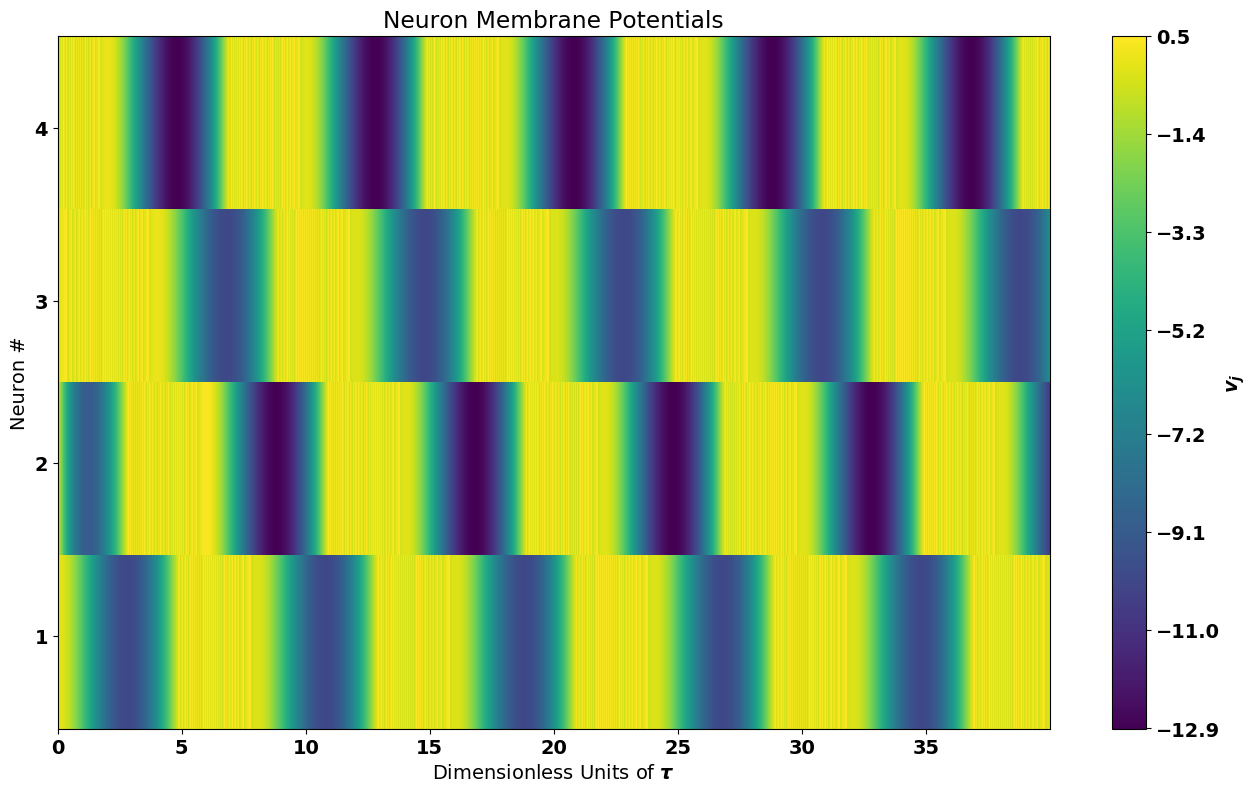
\includegraphics[width=.7\linewidth]{figures/membrane_potential_image.png}
\end{figure}

\newpage

\captionof{figure}{Simulation of equations (\ref{eq:rotated_voltage_dynamics}) and
    (\ref{eq:rho_dot}) with parameters listed in equation (\ref{eq:sim_I_params}). \textbf{\textit{Top:}} The decoded network estimate plotted alongside the target dynamical system. \textbf{\textit{Middle:}} The estimation error along each state-space dimension. \textbf{\textit{Bottom: }}The membrane potentials of the 4 neurons during the same time period.\\
    For the numerical implementation, the matrix exponential was used to integrate the continuous terms over a simulation time step. Continuous terms include all equation terms excepting the delta functions $\omega$ handled separately. After integrating over a timestep, any neuron above threshold was manually reset (action of fast inhibition). If multiple neurons are above threshold, the system is integrated backwards in time until only one neuron is above threshold before spiking. The matrix exponential was computed using a Pad\'{e} approximation via the Python package Scipy: \textit{scipy.linalg.expm()}. 
    } 
    \label{fig:Simulation_I}
\clearpage

\section{Analysis: RMSE vs Spike Rate for Constant Driving Force}




We analyse the network described by equations (\ref{eq:rotated_voltage_dynamics}) and (\ref{eq:rho_dot} for the case of a constant (in time) driving force $c(\xi) = k \mathcal{U}_j$. First we derive explicit expressions for the network estimate, then we compute the resulting RMSE for various driving strengths $k$.\\
\begin{enumerate}
\item Let 
\begin{align*}
A &= -\begin{bmatrix}  
1 & 0 \\
0 & 1
\end{bmatrix},\notag \\
\notag \\
B &= \begin{bmatrix}  
1 & 0 \\
0 & 1
\end{bmatrix}, \notag \\
\notag \\
c(\xi) &= k \mathcal{U}_1 \\
\notag \\
d\xi &= 10^{-4},\notag \\
\notag \\
N &= 4,\notag \\
\notag \\
x(0) &= \begin{bmatrix} \frac{1}{2} & 0 \end{bmatrix}.\notag 
\end{align*}

With the given initial conditions, $v_j = 0$ for $j \neq 1$ for all $\xi$. The dynamics simplify to 
\begin{equation*}
\label{eq:simple_voltage_dynamics_constant_driving}
\dot{v_1} = \Lambda_1 v_1 + (\Lambda_1 + 1)\rho_1 + k - \Omega_1.
\end{equation*}

\item We assume that the decoding matrix D is chosen such that $S_1 = 1$. Because A is the negative identity matrix, it is also clear that $\Lambda_1 = -1$. The preceding equation simplifies to  
\begin{equation}
\label{eq:simple_voltage_dynamics_constant_driving}
\dot{v_1} = -v_1 + k - \Omega_1,
\end{equation}
which is a form of the well-known Leaky Integrate-and-Fire (LIF) model. Assuming a spike has occurred at $v_{th} = \frac{1}{2}$, the voltage has just been reset so that $v_1(0) = -\frac{1}{2}$. Until the next spike, the neuron's trajectory is integrated as 
\begin{align*}
v(\xi) =  k - e^{-\xi} (k + \frac{1}{2}).
\end{align*}

Neglecting any spike reset, the voltage will asymptotically approach $v_1=k$. Thus for any spiking to occur, we must have $k \geq v_{th}$. In this case, the time required to reach a spike threshold $v_{th}$ is 
\begin{align*}
v_{th} &=  k - e^{-\xi_{spike}} (k + \frac{1}{2})
\\
\\
\implies 
e^{-\xi_{spike}} &=  \frac{k - v_{th}}{k + \frac{1}{2}}
\\
\\
&= \frac{1 - \frac{v_{th}}{k}} {1 + \frac{1}{2k}}\\
\\
 \implies
 \xi_{spike} &= - ln
 \left(
 \frac{1 - \frac{v_{th}}{k}} {1 + \frac{1}{2k}}
  \right)
 \\
 \\
 \implies 
 \frac{1}{\xi_{spike}} &= - \frac{1}{ 
 ln
 \left(
 \frac{1 - \frac{v_{th}}{k}} {1 + \frac{1}{2k}}
  \right)
 } \\
 \\
 &=   \frac{1}{ 
 ln \left(
  1 + \frac{1}{2k}
  \right) 
  -
 ln
 \left(
 1 - \frac{v_{th}}{k}\right),
 }
\end{align*}
which determines the frequency  at which the LIF neuron spikes.  Denote this frequency as a function of driving strength $k$ by $\phi(k)$:
\begin{align}
\label{eq:freq_vs_driving_strength_const}
\phi(k) \overset{\Delta}{=}  \frac{1}{ 
 ln \left(
  1 + \frac{1}{2k}
  \right) 
  -
 ln
 \left(
 1 - \frac{v_{th}}{k}\right)
 }.
\end{align}
\\

\begin{figure}
\centering
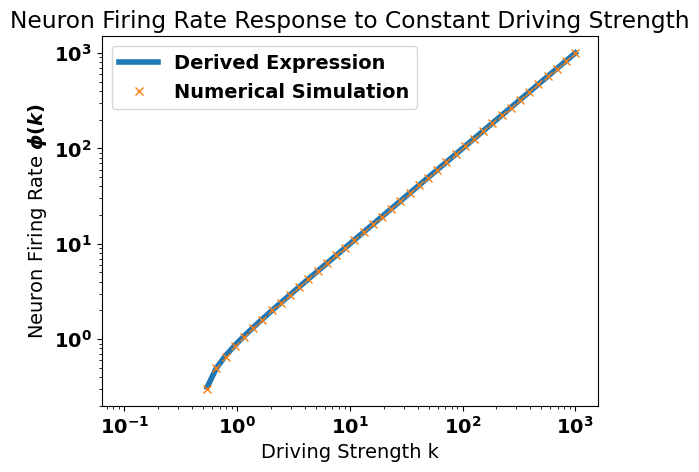
\includegraphics[width=\linewidth]{figures/phi_vs_k_const_driving.png}
\caption{A log-log plot of equation (\ref{eq:freq_vs_driving_strength_const}) alongside the rates measured from numerical simulations. The simulation parameters are described at the beginning of this section, with the decoder matrix $D$ chosen to be the first d rows of the N x N identity matrix. This ensures the singular values $S_j = 1$ as assumed in the derivation.   The rate was measured as the number of spike resets divided by the duration of the simulation. }\label{fig:spike_rate_vs_k_const_driving}
\end{figure}

The network will encode the constant driving force by spiking at a fixed rate determined by equation $(\ref{eq:freq_vs_driving_strength_const})$. Figure (\ref{fig:spike_rate_vs_k_const_driving}) shows a plot of equation (\ref{eq:freq_vs_driving_strength_const}) along with numerically computed spike rates for a simulated network driven with constant drive strength $k$.  Similar to membrane voltage, the resulting PSC and readout dynamics are reduced to one neuron periodically spiking:
\begin{align*}
\dot{\rho_1} &= -\rho_1 + \Omega_1 \\ 
\\
\implies 
\dot{\hat{x}} &= - \mathcal{U}_1 \rho_1 + \mathcal{U}_1 \Omega_1\\
\\ 
&= - \hat{x} + \mathcal{U}_1 \Omega_1. 
\end{align*}



\item The spike train $\Omega_1$ is a periodic sequence of impulses spaced in time by $\frac{1}{\phi(k)}$. Hence $\Omega_1(\xi) = \sum_{l=0}^{\infty} \delta \left(\xi - \frac{l}{\phi(k)}\right).$
The network estimate therefore has dynamics
\begin{align}
\label{eq:estimation_dynamics_const_driving}
\dot{\hat{x}} &= -\hat{x}  + \mathcal{U}_1 \sum_{l=0}^{\infty} \delta \left(\xi - \frac{l}{\phi(k)}\right).
\end{align}

The target dynamical system is
\begin{align*}
\dot{x} = - x + k 
 \mathcal{U}_1 \\
 x(0) = \begin{bmatrix} \frac{1}{2} & 0 \end{bmatrix},
\end{align*}
which has a stable fixed point at
\begin{align}
\label{eq:steady_state_dynamics_const_driving}
x = k \mathcal{U}_1.
\end{align}

\item Equation (\ref{eq:estimation_dynamics_const_driving}) implies that the network estimate $\hat{x}$ will decay until the first spike $\xi_1^1$ occurs:
\begin{align*}
\hat{x}(\xi) = x(0) e^{-\xi}, \hspace{4mm} 0 \leq \xi < \frac{1}{\phi(k)}.
\end{align*}


 At this instant, the vector $\mathcal{U}_1$ is added to the network estimate.
 \begin{align*}
 \hat{x}( \frac{1}{\phi(k)}) =  x(0) e^{- \frac{1}{\phi(k)}} + \mathcal{U}_1.
 \end{align*}
 
Decay again occurs until the next spike
\begin{align*}
\hat{x}(\xi) &= \hat{x}(\frac{1}{\phi(k)}) e^{-(\xi - \frac{1}{\phi(k)})}, \\
\\
&= \left( x(0) e^{- \frac{1}{\phi(k)}} + \mathcal{U}_1 \right)e^{-(\xi - \frac{1}{\phi(k)})} , \hspace{4mm} 
\frac{1}{\phi(k)} \leq \xi < \frac{2}{\phi(k)}\\
\\
\implies
\hat{x}(\frac{2}{\phi(k)}) &= \left( x(0) e^{- \frac{1}{\phi(k)}} + \mathcal{U}_1 \right) e^{-(\frac{1}{\phi(k)})} + \mathcal{U}_1\\
\\
&= x(0)
e^{-\frac{2}{\phi(k)}} + \mathcal{U}_1 e^{-\frac{1}{\phi(k)}} 
+ \mathcal{U}_1.
\end{align*}

The third spike more clearly shows the recursive behavior
\begin{align*}
\hat{x}(\frac{3}{\phi(k)}) &= \left[x(0)
e^{-\frac{2}{\phi(k)}} + \mathcal{U}_1 e^{-\frac{1}{\phi(k)}} 
+ \mathcal{U}_1\right] e^{-\frac{1}{\phi(k)}} + \mathcal{U}_1\\
\\
&= x(0) e^{-\frac{3}{\phi(k)}} + \mathcal{U}_1 e^{-\frac{2}{\phi(k)}} 
+ \mathcal{U}_1 e^{-\frac{1}{\phi(k)}} + \mathcal{U}_1
\end{align*}
Let us consider the $n^{th}$ spike sufficiently far from $\xi=0$ such that the transient term $x(0)e^{-\frac{n}{\phi(k)}}$ can be neglected. This leads to the expression

\begin{align*}
\hat{x}(\frac{n}{\phi(k)}) &= \sum_{l=0}^{n-1} \mathcal{U}_1 e^{- \frac{l}{\phi(k)}}  \\
\\
&= \mathcal{U}_1 \frac
{ 1 - e^{-\frac{n}{\phi(k)}}  }
{ 1 - e^{-\frac{1}{\phi(k)}}  }.
\end{align*}

For sufficiently large $n$, this converges to 
\begin{align}
\label{eq:steady_state_estimate_const_driving}
\hat{x}(\xi_1^n) = \frac{\mathcal{U}_1}{1 - e^{-\frac{1}{\phi(k)}}}.
\end{align}


\begin{figure}[h]
\centering
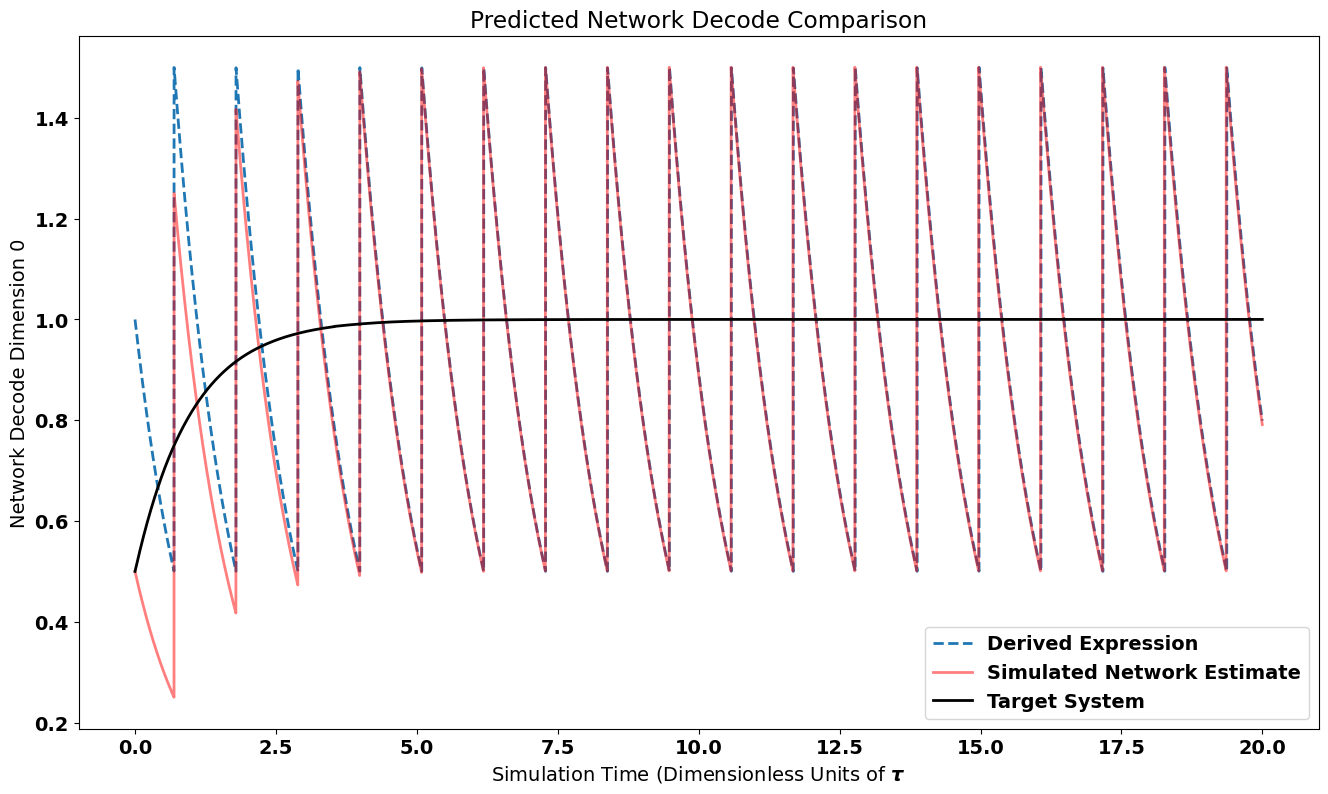
\includegraphics[width=\linewidth]{figures/network_decode_long_term_estimate_const_driving.png}
\caption{Comparison of the derived long-term network estimate equation (\ref{eq:const_driving_network_estimate_explicit_expression_long_term}) to numerical simulation. Parameters are the same as the previous figure, with $k = 1$.}
\label{fig:const_driving_convergence_to_derived_spike_readout}
\end{figure}

\item The preceding argument states that after a transient interval, the network estimate at any spike time $\xi_1^n$ is given by equation (\ref{eq:steady_state_estimate_const_driving}). As shown in figure (\ref{fig:const_driving_convergence_to_derived_spike_readout}), this convergence occurs after roughly 5 spikes for the case $k = 1$. 


We know from equation (\ref{eq:estimation_dynamics_const_driving}) that the estimate will decay exponentially from this value over an interval $\frac{1}{\phi(k)}$ until a spike returns it returns to the initial value. Thus the network estimate between two consecutive spikes is given by 
\begin{align*}
\hat{x}(\xi) = \frac{\mathcal{U}_1}{1 - e^{-\frac{1}{\phi(k)}}} e^{-(\xi - \xi_1^n)}, \hspace{4mm} 0 \leq \xi - \xi_1^n  < \frac{1}{\phi(k)}.
\end{align*}

Combine this expression with equation (\ref{eq:steady_state_estimate_const_driving}), we have an explicit expression for the long-term behavior of the network estimate given by 

\begin{equation}
\label{eq:const_driving_network_estimate_explicit_expression_long_term}
\hat{x}(\xi) =
\frac{\mathcal{U}_1}{1 - e^{-\frac{1}{\phi(k)}}} e^{- (\xi - \xi_1^1) \mod{\frac{1}{\phi(k)}}},
\end{equation} 
where $x \mod{y}$ denotes the fractional remainder of $x$ after division by $y$. 

\clearpage

\item Assume the true system dynamics have settled to their fixed point $x = k \mathcal{U}_1$. From equation (\ref{eq:const_driving_network_estimate_explicit_expression_long_term}) the network estimate $\hat{x}$ and therefore error $e = x - \hat{x}$ is a periodic function of $\xi$ with period $\frac{1}{\phi(k)}$. The RMSE over any integer number of spike periods is easily calculated from the RMSE over a single spike period. 

We compute the per-spike RMSE of the error signal  $e$ by 
\begin{equation}
\label{eq:per_spike_rmse_def}
RMSE_{spike} \overset{\Delta}{=} \sqrt{\phi(k) \int_{0}^{\frac{1}{\phi(k)}} \!  ||e(\tau)||^2 \, \, \mathrm{d}\tau}.
\end{equation}

The integrand $||e(\tau)||^2$ simplifies to 

\begin{align*}
e^T e &= (x - \hat{x})^T (x - \hat{x}) \\
\\
&= x^T x - 2 x^T \hat{x} + \hat{x}^T \hat{x} \\
\\
&= k^2 \, \mathcal{U}_1 ^T \mathcal{U}_1 - 2 k \, \,  \mathcal{U}_1^T \mathcal{U}_1 \frac{e^{- \tau}}{1 - e^{-\frac{1}{\phi(k)}}} 
+ 
\mathcal{U}_1^T \mathcal{U}_1  \left(\frac{e^{- \tau}}{1 - e^{-\frac{1}{\phi(k)}}} \right)^2\\
\\
&= k^2 - \frac{ 2 k \, e^{- \tau}}{1 - e^{-\frac{1}{\phi(k)}}} 
+ 
\frac{e^{- 2\tau}}{\left(1 - e^{-\frac{1}{\phi(k)}}\right)^2}.
\end{align*}

Therefore the integral is

\begin{align*}
\phi(k)\int_{0}^{\frac{1}{\phi(k)}} \!  ||e(\tau)||^2 \, \, \mathrm{d}\tau &= 
\phi(k)\int_{0}^{\frac{1}{\phi(k)}} \!  
k^2 - \frac{ 2 k \, e^{- \tau}}{1 - e^{-\frac{1}{\phi(k)}}} 
+ 
\frac{e^{- 2\tau}}{\left(1 - e^{-\frac{1}{\phi(k)}}\right)^2}
\, \, \mathrm{d}\tau\\
\\
&= k^2 + \phi(k) \frac{2 k }{1 - e^{-\frac{1}{\phi(k)}}} \left( e^{- \frac{1}{\phi(k)}} - 1 \right) 
- \phi(k) \frac{1}{ 2 \, \left(1 - e^{-\frac{1}{\phi(k)}}\right)^2} 
\left( e^{ -  \frac{2}{\phi(k)}} - 1 \right) \\
\\
&= k^2  + \phi(k) \left[ \frac{1 - e^{-\frac{2}{\phi(k)}}}{2 \left(1 - e^{-\frac{1}{\phi(k)}} \right)^2}  -2 k \right]  .
\end{align*}


The per-spike RMSE of the network estimate as a function of drive strength $k$ is therefore
\begin{equation}
\label{eq:per_spike_rmse_const_driving_k}
RMSE_{spike}(k) =
\sqrt{k^2  + \phi(k) \left[ \frac{1 - e^{-\frac{2}{\phi(k)}}}{2 \left(1 - e^{-\frac{1}{\phi(k)}} \right)^2}  -2 k \right] }.
\end{equation}

To write the RMSE explicitly as a function of firing rate $\phi(k)$, we invert equation (\ref{eq:freq_vs_driving_strength_const}) to obtain
\begin{align*}
k(\phi)&=  \frac{ v_{th} + \frac{e^{-\frac{1}{\phi}}}{2}}{1 - e^{-\frac{1}{\phi}}}.
\end{align*}

Substitute this for k to obtain

\begin{align}
\label{eq:per_spike_rmse_const_driving_phi}
RMSE_{spike}(\phi) &=
\sqrt{k(\phi)^2  + \phi \left[ \frac{1 - e^{-\frac{2}{\phi}}}{2 \left(1 - e^{-\frac{1}{\phi}} \right)^2}  -2 k(\phi) \right] } \notag
%
\\ 
\\
%
&= 
\sqrt{
     \left(
		     \frac
			{
			v_{th} + \frac{e^{- \frac{1}{\phi}      }}{2}
			}
			{
			1 - e^{-\frac{1}{\phi}   }
			}
      \right)^2
  +
   \phi \left[ \frac{1 - e^{-\frac{2}{\phi}}}{2 \left(1 - e^{-\frac{1}{\phi}} \right)^2}  
   -2 \, 
			    \frac
			{
			v_{th} + \frac{e^{-\frac{1}{\phi}   }}{2}
			}
			{
			1 - e^{-\frac{1}{\phi}   }
			}
     \right]
     } \notag.
\end{align}

Equations (\ref{eq:per_spike_rmse_const_driving_k}) and (\ref{eq:per_spike_rmse_const_driving_phi}) are plotted in figure (\ref{fig:const_driving_per_spike_rmse_vs_phi_k}). Note that the drive strength varies the amplitude of the target system's steady state. Thus we have derived the the network performance over its dynamic range of representable state space. 



\begin{figure}[h]
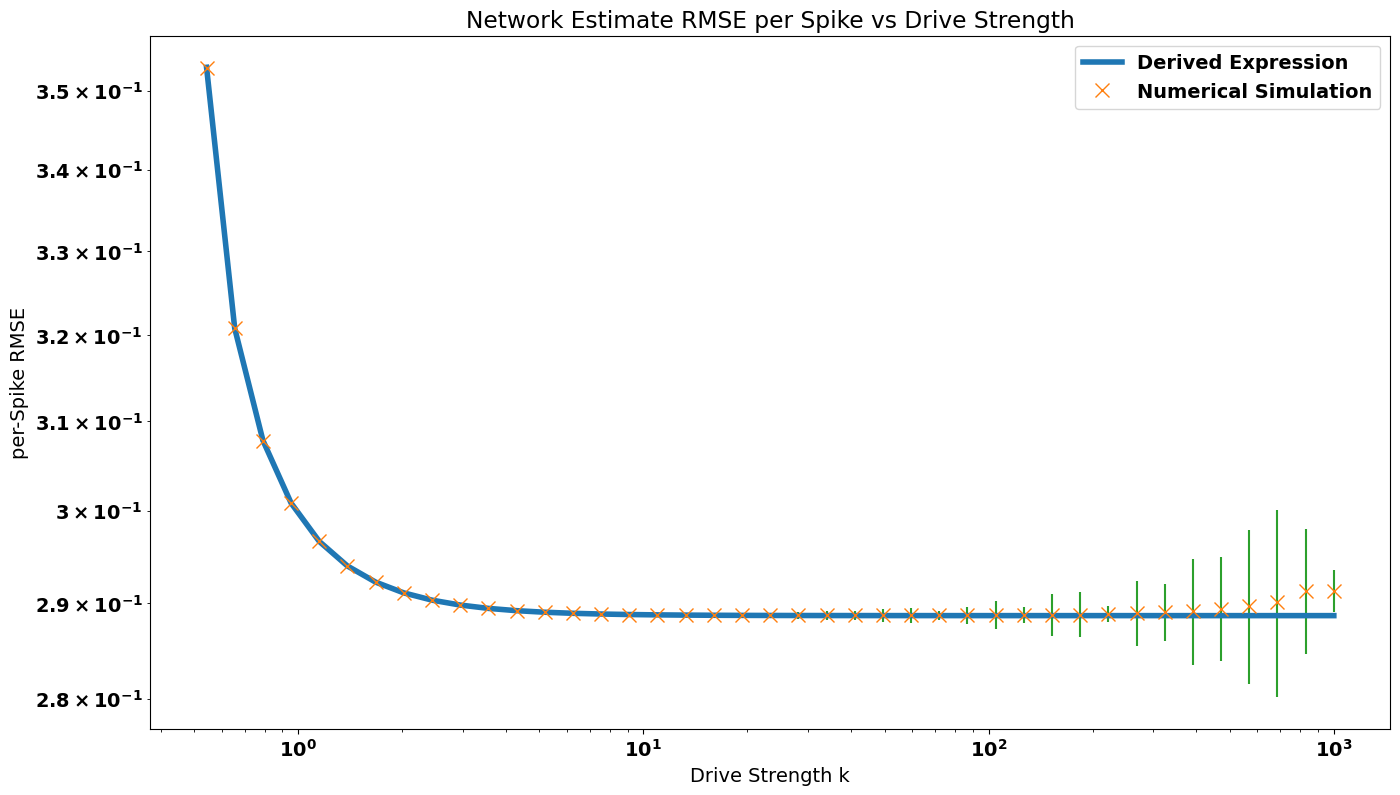
\includegraphics[width=\linewidth]{figures/rmse_sp_vs_k_const_driving.png}
\centering
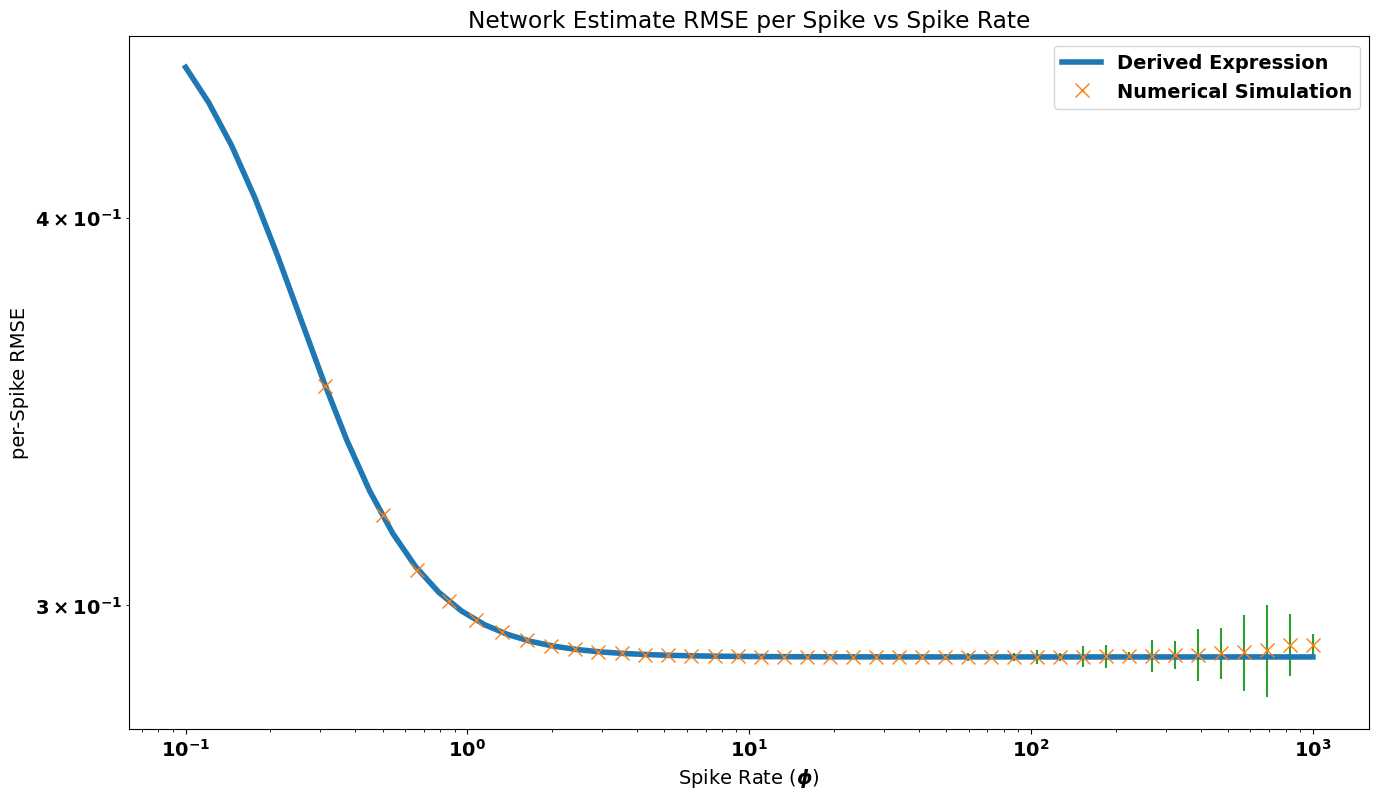
\includegraphics[width=\linewidth]{figures/rmse_sp_vs_phi_const_driving.png}
\caption{\textbf{\textit{Top:}} A log-log plot of equation (\ref{eq:per_spike_rmse_const_driving_k}). \textbf{\textit{Bottom:}} A log-log plot of equation (\ref{eq:per_spike_rmse_const_driving_phi}). \textbf{\textit{Both:}} Each simulated data point is the RMSE averaged over all inter-spike intervals in a simulation of length $T = 80 \tau_s$ at a constant (in time) drive strength. Between simulations, the spike rates were varied by sweeping drive strength. Green vertical lines towards the larger values are +/- 1 standard deviation. The spike rates $\hat{\phi}$ were computed numerically via dividing the number of spikes in a simulation by the simulation duration. The RMSE between two adjacent spikes was computed by numerical integration as a discrete sum: $\hat{RMSE} = \sqrt{\hat{\phi} \sum_{\tau \text{ between spikes }} e(\xi)^T e(\xi) \, \, d\xi }$. The increase in standard deviation is due to finite approximation error from numerical integration.}
\label{fig:const_driving_per_spike_rmse_vs_phi_k}
\end{figure}
\end{enumerate}

\clearpage


\section{Analysis: RMSE vs Spike Rate for a Fixed Dynamical System}
\label{section:analysis:rmse_vs_spike_rate_constant_dynamics}

 Here we derive the RMSE of a signal representing a given dynamical system with a varying spike rate. The RMSE is computed over a constant interval of time for a fixed target system while the spike rate is varied.  
\begin{enumerate}
\item Our system is described by 

\begin{align*}
A &= -\begin{bmatrix}  
1 & 0 \\
0 & 1
\end{bmatrix},\notag \\
\notag \\
B &= \begin{bmatrix}  
1 & 0 \\
0 & 1
\end{bmatrix}, \notag \\
\notag \\
c(\xi) &= \mathcal{U}_1 \\
\notag \\
d\xi &= 10^{-4},\notag \\
\notag \\
N &= 4,\notag \\
\notag \\
x(0) &= \begin{bmatrix} \frac{1}{2} & 0 \end{bmatrix}.\notag 
\end{align*}

\item With the given initial conditions, $v_j = 0$ for $j \neq 1$ for all $\xi$. From equations (\ref{eq:rotated_voltage_psc_def}) and (\ref{eq:rotated_voltage_dynamics}), the dynamics simplify to 
\begin{equation*}
\dot{v_1} = \Lambda_1 v_1 + (\Lambda_1 + 1)\rho_1 + S_1 \mathcal{U}_1^T \mathcal{U}_1 - \Omega_1.
\end{equation*}

It is clear that $\Lambda_1 = -1$ so that 
\begin{equation}
\label{eq:analysis_voltage_dynamics_constant_driving_const_dynamics}
\dot{v_1} = -v_1 + S_1 - \Omega_1,
\end{equation}
which is a form of the well-known Leaky Integrate-and-Fire (LIF) model.
\item  Assuming a spike has occurred at $v_{th} = \frac{1}{2}$, the voltage has just been reset so that $v_1(0) = -\frac{1}{2}$. Until the next spike, the neuron's trajectory is integrated as 
\begin{align*}
v(\xi) =  S_1 - e^{-\xi} (S_1 + \frac{1}{2}).
\end{align*}

The spike occurs at $v(\xi_{spike}) = v_{th}$ or 
\begin{align*}
v_{th} &= S_1 - e^
{
	-\xi
}
(
	S_1 + \frac		
		  {
			  1
		  }
		  {
			  2
		  }
 ) 
%
\\
\\
%
\implies 
\frac
{
	S_1 - v_{th}  
}
{
	S_1 + \frac
		  {
		       1
		  }
		  {
		  	   2
		  }
}
&=
e^
{
	-\xi_{spike}
}
%
\\
\\
%
\implies
\xi_{spike}
&= 
ln
(
	S_1 + \frac
			{
				1
			}
			{
				2
			}
)
- 
ln
(
	S_1 - v_{th}
).
\end{align*}

The inverse of the preceding expression gives the firing rate of the neuron,

\begin{align}
\label{eq:analysis_const_dynamics_phi_vs_s}
\phi(S_1)
\overset{\Delta}{=}
\frac
{
	1
} 
{
	ln
	(
		1 + \frac
				{
					1
				}
				{
					2 \, S_1
				}
	)
	- 
	ln
	(
		1 - \frac
			{
				v_{th}
			}
			{
				S_1
			}
	)
}.
\end{align}

Equation (\ref{eq:analysis_const_dynamics_phi_vs_s}) describes the neuron's firing rate as a function of the decode matrix $D$'s singular values. Thus for a given target dynamical system, the decode matrix $D$ determines the neuron's firing rates. 

\item From equations (\ref{eq:rho_dot}) and (\ref{eq:xhat}),
\begin{align}
\label{eq:analysis:constant_driving_constant_dynamics_estimate_equation_implicit}
\dot
{
	\rho
}
&= 	- \rho  + \Omega \notag
% 
\\ \notag
\\ \notag
%
\implies
\dot{
	\hat
	{
		x
	}
}
&= 
-\hat
{
	x
}
+ \mathcal{U} \Omega
% \notag
\\ \notag
\\ 
%
\implies
\dot
{
	\hat
	{
		x
	}
}
&= 
-\hat
{
	x
}
+
\mathcal
{
	U
}_1 
\sum_
{
	l=0
}
^
{
	\infty
}
\delta 
\left(
	\xi - \frac
		  {
			  l
		  }
		  {
			  \phi
		  }
\right),
\end{align}
where the last equality follows from the periodicity of the LIF neuron firing at rate $\phi$.

We solve equation (\ref{eq:analysis:constant_driving_constant_dynamics_estimate_equation_implicit}) and inductively derive an explicit expression for its asymptotic behavior in time. Note that equation (\ref{eq:analysis:constant_driving_constant_dynamics_estimate_equation_implicit}) implies that the network estimate $\hat{x}$ will decay until the first spike $\xi_1^1$ occurs:
\begin{align*}
\hat{x}(\xi) = x(0) e^{-\xi}, \hspace{4mm} 0 \leq \xi < \xi_1^1.
\end{align*}


 At this instant, the  vector $\mathcal{U}_1$ is added to the network estimate,
 \begin{align*}
 \hat{x}( \xi_1^1) =  x(0) e^{-\xi_1^1 } + \mathcal{U}_1.
 \end{align*}
 
Decay again occurs until the next spike
\begin{align*}
\hat{
	x
}
(
	\xi
)
&= \hat
{
	x
}
(
	\xi_{1}^1
)
e^
{
	-
	(
		\xi - \xi_{1}^1
	)
},
%
\\
\\
%
&=
\left(
	 x(0) e^
	 {
	 	-\xi_1^1
	 }
	 +
	 \mathcal{U}_1
\right)
e^
{
	-
	(
		\xi - 
		\xi_1^1
	)
} , \hspace{4mm} 
0 \leq \xi - \xi_1^1 <
\frac
{
	1
}
{
	\phi
}
%
\\
\\
%
\implies
\hat
{
	x
}
(
	\xi_1^1 + 
	\frac
	{
		1
	}
	{
		\phi
	}
)
&=
\left(
	x
	(
		0
	)
	e^
	{
		- \xi_1^1
	}
	 +
	 \mathcal{U}_1 
\right)
e^
{
	-
	\frac
	{
		1
	}
	{
		\phi
	}
}
+
\mathcal{U}_1
\\
\\
&=
x
(
	0
)
e^
{	
	-\left(
		\xi_1^1 + 
		\frac
		{
			1
		}
		{
			\phi
		}
	\right)
}
+
\mathcal{U}_1
e^
{
	-\frac
	{
		1
	}
	{
		\phi
	}
} 
+
\mathcal{U}_1.
\end{align*}

The third spike more clearly shows the recursive behavior
\begin{align*}
\hat
{
	x
}
(
	\xi_1^1 + 
	\frac
	{
		2
	}
	{
		\phi
	}
)
&= 
\left[
	x
	(
		0
	)
	e^
	{	
		-\left(
			\xi_1^1 + 
			\frac
			{
				1
			}
			{
				\phi
			}
		\right)
	}
	+
	\mathcal{U}_1
	e^
	{
		-\frac
		{
			1
		}
		{
			\phi
		}
	} 
	+
	\mathcal{U}_1.
\right]
e^
{
	-\frac
	{
		1
	}
	{
			\phi
	}
}
+
\mathcal{U}_1 
%
\\
\\
%
&= 
x
(
	0
)
e^
{	
	-\left(
		\xi_1^1 + 
		\frac
		{
			2
		}
		{
			\phi
		}
	\right)
}
+
\mathcal{U}_1
e^
{
	-\frac
	{
		2
	}
	{
		\phi
	}
} 
+
\mathcal{U}_1
e^
{
	-\frac
	{
		1
	}
	{
			\phi
	}
}
+
\mathcal{U}_1.
\end{align*}
Let us consider the $n^{th}$ spike sufficiently far from $\xi=0$ such that the transient term $
x
(
	0
)
e^
{
	-\left(
		\xi_1^1	+ 
		\frac
		{
			n-1
		}
		{
			\phi
		}
	\right)
}
$ can be neglected. This leads to the expression

\begin{align*}
\hat
{
	x
}
\left(
	\xi_1^1 + 
	\frac
	{
		n
	}
	{
		\phi
	}
\right)
&=
\sum_
{
	l=0
}
^
{
n-1
}
\mathcal{U}_1
e^
{
	- \frac
	{
		l
	}
	{
		\phi
	}
}
%
\\
\\
%
&=
\mathcal{U}_1
\frac
{
	1 - e^
	{
		-\frac
		{
			n
		}
		{
			\phi
		}
	}  
}
{
	1 - e^
	{
		-\frac
		{
			1
		}
		{
			\phi
		}
	}  
}.
\end{align*}

For sufficiently large $n$, this converges to 
\begin{align*}
\hat
{
	x
}
\left(
	\xi_1^1 + \xi_1^n
\right)
&=
\frac
{
	\mathcal{U}_1
}
{
	1 - e^
	{
		-\frac
		{
			1
		}
		{
			\phi
		}
	}
}.
\end{align*}

Between two spikes, the dynamics are exponential decay
\begin{align*}
\hat{
	x
}
\left(
	\xi
\right)
&=
\frac
{
\mathcal{U}_1
}
{
	1 - e^
	{
		-\frac
		{
			1
		}
		{
			\phi
		}
	}
}
e^
{
	-\left(
		\xi - \xi_1^n
	\right)
}
,
\hspace{4mm}
0 \leq \xi - \xi_1^n  < 
\frac
{
	1
}
{
	\phi
,}
\end{align*}
so that the long term network estimate is
\begin{align*}
\label{eq:analysis:constant_driving_constant_dynamics_estimate_equation_implicit}
\hat{
x
}
\left(
	\xi
\right)
&=
\frac
{
	\mathcal{U}_1
}
{
	1 - e^
	{
		-\frac
		{
			1
		}
		{
			\phi
		}
	}
}
e^
{
	- (\xi - \xi_1^1) 
	\mod
	{
		\frac
		{
			1
		}
		{
			\phi
		}
	}
}.
\end{align*}

Applying equation (\ref{eq:analysis_const_dynamics_phi_vs_s}),

\begin{align*}
e^
{
	-\frac
	{
		1
	}
	{
		\phi
	}
}
&= 
e^
{
	ln
	\left(
		1 - 
		\frac
		{
			v_{th}
		}
		{
			S_1	
		}
	\right)
	-
	ln
	\left(
			1 +
		\frac
		{
			1
		}
		{
			2 \, S_1	
		}	
	\right)
}
%
\\
\\
%
&= 
\frac
{
	1 - 
	\frac
	{
		v_{th}
	}
	{
		S_1	
	}
}
{
	1 +
	\frac
	{
		1
	}
	{
		2 \, S_1	
	}	
}
%
\\
\\
%
\implies
1 - e^
{
	-\frac
	{
		1
	}
	{
		\phi
	}
}
&= 
1 - 
\frac
{
	1 - 
	\frac
	{
		v_{th}
	}
	{
		S_1	
	}
}
{
	1 +
	\frac
	{
		1
	}
	{
		2 \, S_1	
	}	
}
%
\\
\\
%
&= 
\frac
{
	1 + 
	\frac
	{
		1
	}
	{
		2 \, S_1
	}
	-
	1 + 
	\frac
	{
		v_{th}
	}
	{
		S_1
	}
}
{
	1 + 
	\frac
	{
		1
	}
	{
		2 \, S_1
	}
}
%
\\
\\
%
&= 
\frac
{
	\frac
	{
		1
	}
	{
		S_1
	}
	\left(
		\frac
		{
			1
		}
		{
			2
		}
		+ v_{th}
	\right)	
}
{
	1 + 
	\frac
	{
		1
	}
	{
		2 \, S_1
	}
}
%
\\
\\
%
&= 
\frac
{
	\frac
	{
		1
	}
	{
		2
	}
	+ v_{th}
}
{
	S_1 + 
	\frac
	{
		1
	}
	{
		2
	}
}s
%
\\
\\
%
\implies 
\frac
{
	S_1^
	{
		-1
	}
}
{
	1 - e^
	{
		-\frac
		{
			1
		}
		{
			\phi
		}
	}
} 
&=
\frac
{
	1
}
{
	S_1
}
\frac
{
	S_1 + 
	\frac
	{
		1
	}
	{
		2
	}
}
{
	\frac
	{
		1
	}
	{
		2
	}
	+ v_{th}
}
%
\\
\\
%
&= 
\frac
{
	1 + 
	\frac
	{
		1		
	}
	{
		2 \, S_1
	}
}
{
	\frac
	{
		1
	}
	{
		2
	}
	+
	v_{th}
}
%
\\
\\
%
&= 
1 +
\frac
{
	1
}
{
	2 \, S_1
}
, 
\end{align*}
where the last equality uses the fact that $v_{th} = \frac{1}{2}$.  
The network estimate is therefore
\begin{equation}
\label{eq:analysis:constant_driving_constant_dynamics_estimate_equation_explicit}
\hat
{
	x
}
(
	\xi
)
= 
\left(
1 + 
\frac
{
	1
}
{
	2 \, S_1
}
\right)
e^
{
	- \hspace{2mm}
	\left(
		\xi - \xi_1^1
	\right)
	\mod
	{
		\frac
		{
			1
		}
		{
			\phi
		}
	}
}
\, \, \mathcal{U}_1
\end{equation}

Equation (\ref{eq:analysis:constant_driving_constant_dynamics_estimate_equation_explicit}) is plotted in figure (\ref{fig:analysis:constant_driving_constant_dynamics_explicit_vs_simulation_comparison}). The trajectories converge indefinitely at $\tau \simeq 5$.

\begin{figure}
\centering
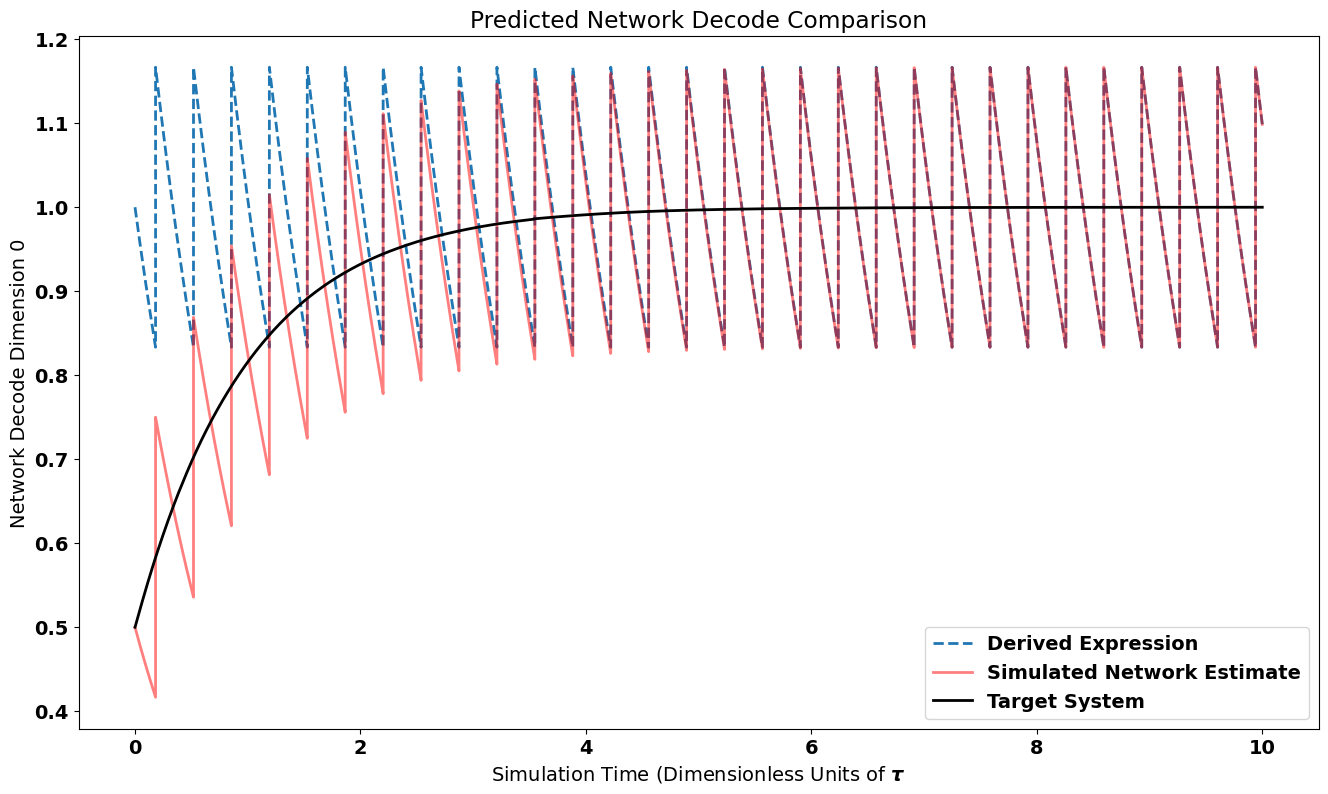
\includegraphics[width=\linewidth]{figures/analysis_const_dynamics_const_driving_network_decode_explicit_comparison.png}
\caption{Comparison of the derived long-term network estimate equation (\ref{eq:analysis:constant_driving_constant_dynamics_estimate_equation_explicit}) to numerical simulation. The simulation parameters are described at the beginning of this section, with the decoder matrix $D$ chosen to be the first $d=2$ rows of the N x N identity matrix, scaled by $3$. This ensures the singular value $S_1 = 3$. Using the rate computed by equation (\ref{eq:analysis_const_dynamics_phi_vs_s}), the derived estimate is computed then overlaid on the numerical simulation after offsetting time by the first spike arrival, $\xi_1^1$. }
\label{fig:analysis:constant_driving_constant_dynamics_explicit_vs_simulation_comparison}
\end{figure}



\item Suppose the systems have settled so that equation (\ref{eq:analysis:constant_driving_constant_dynamics_estimate_equation_explicit}) holds. To compute the RMSE of the estimate, consider the interval between two successive spikes. The RMSE over this period is
\begin{equation*}
RMSE_{spike} \overset{\Delta}{=}\
\sqrt
{
	\phi \int_
	{	
		0
	}
	^
	{
		\frac
		{
			1
		}
		{
			\phi
		}
	}
	 \!  e^T e(\tau)\, \, \mathrm{d} \tau
}.
\end{equation*}


Note that the target dynamical system settles to a fixed point $x = \mathcal{U}_1$ so that
\begin{align*}
e(\tau) &= x(\tau) -
 \hat
 {
 	x
 }
 (
 	\tau
 )
%
\\
\\
%
&= 
\mathcal{U}_1 - 
\left(
	1 + 
	\frac
	{
		1
	}
	{
		2 \, S_1
	}
\right)
e^
{
	- \tau
}
\, \, \mathcal{U}_1
%
\\
\\
%
&= 
\mathcal{U}_1 
\left[
	1 - e^
	{
		-\tau
	}
	\left(
		1 + 
		\frac
		{
			1
		}
		{
			2 \, S_1
		}
	\right)
\right]
%
\\
\\
%
\implies
e^T e
\left(
\tau
\right)
&=
\left[
	1 - e^
	{
		-\tau
	}
	\left(
		1 + 
		\frac
		{
			1
		}
		{
			2 \, S_1
		}
	\right)
\right]^2
%
\\
\\
%
&= 
1 - 2 \, e^
{
	-\tau
}
\left(
	1 + 
	\frac
	{
		1
	}
	{
		2 \, S_1
	}
\right)
+
e^
{
	-2 \, \tau
}
\left(
	1 + 
	\frac
	{
		1
	}
	{
		S_1
	}
	+
	\frac
	{
		1
	}
	{
		4 \, S_1^2
	}
\right).
\end{align*}
The integral is therefore 

\begin{align*}
	\int_
	{	
		0
	}
	^
	{
		\frac
		{
			1
		}
		{
			\phi
		}
	}
	 \!  e^T e(\tau)\, \, \mathrm{d} \tau 
	 &= 
	 \frac
	 {
	 	1
	 }
	 {
	 	\phi
	 }
	 -
	 2
	 \left(
	 	1 + 
	 	\frac
	 	{
	 		1
	 	}
	 	{
	 		2 \, S_1
	 	}
	 \right)
	\frac
	{
		\frac
		{
			1
		}
		{
			2
		}
		+ v_{th}
	}
	{
		S_1 + 
		\frac
		{
			1
		}
		{
			2
		}
	}
	+
	\frac
	{
		1
	}
	{
		2
	}
	\left(
		1 + 
		\frac
		{
			1
		}
		{
			S_1
		}
		+
		\frac
		{
			1
		}
		{
			4 \, S_1^2
		}
	\right)
	\left(
		1 - 
		e^
		{
			\frac
			{
				2
			}
			{
				\phi
			}
		}		
	\right)
	%
	\\
	\\
	%
	&= 
	 \frac
	 {
	 	1
	 }
	 {
	 	\phi
	 }
	 -
	 2
	 \frac
	 {
	 	1
	 }
	 {
	 	S_1
	 }
	 \left(
	 	S_1 + 
	 	\frac
	 	{
	 		1
	 	}
	 	{
	 		2
	 	}
	 \right)
	\frac
	{
		\frac
		{
			1
		}
		{
			2
		}
		+ v_{th}
	}
	{
		S_1 + 
		\frac
		{
			1
		}
		{
			2
		}
	}
	+
	\frac
	{
		1
	}
	{
		2
	}
	\left(
		1 + 
		\frac
		{
			1
		}
		{
			S_1
		}
		+
		\frac
		{
			1
		}
		{
			4 \, S_1^2
		}
	\right)
	\left(
		1 - 
		e^
		{
			\frac
			{
				2
			}
			{
				\phi
			}
		}		
	\right)
		%
	\\
	\\
	%
	&= 
	 \frac
	 {
	 	1
	 }
	 {
	 	\phi
	 }
	 -
	 \frac
	 {
	 	1 + 2\, v_{th}
	 }
	 {
	 	S_1
	 }
	+
	\frac
	{
		1
	}
	{
		2
	}
	\left(
		1 + 
		\frac
		{
			1
		}
		{
			S_1
		}
		+
		\frac
		{
			1
		}
		{
			4 \, S_1^2
		}
	\right)
	\left(
		1 - 
		e^
		{
			\frac
			{
				2
			}
			{
				\phi
			}
		}		
	\right),
	%
	\\
	\\
	%
	&= 
	 \frac
	 {
	 	1
	 }
	 {
	 	\phi
	 }
	 -
	 \frac
	 {
	 	1 + 2\, v_{th}
	 }
	 {
	 	S_1
	 }
	+
	\frac
	{
		1
	}
	{
		2
	}
	\frac
	{
		1
	}
	{
		S_1
	} 
	\left(
		1 + 
		\frac
	{
			1
		}
		{
			4 \, S_1
		}
		+ 
		2\, v_{th}
		-
		\frac
		{
			v_{th}^2
		}
		{
			S_1
		}
	\right)
	%
	\\
	\\
	%
	&= 
	\frac
	{
		1
	}
	{
		\phi
	}
	-
	\frac
	{
		1 + 2 \, v_{th} -
		\frac
		{
			1
		}
		{
			S_1
		}
		\left(
			\frac
			{
				1
			}
			{
				4
			}
			- v_{th}^2
		\right)
	}
	{
		2 \, S_1
	}	
	%
	\\
	\\
	%
	&= 
	\frac
	{
		1
	}
	{
		\phi
	}
	- \frac
	{
		1
	}
	{
		S_1
	},
\end{align*}
where we have used the earlier result
\begin{align*}
\frac
{
	S_1^
	{
		-1
	}
}
{
	1 - e^
	{
		\frac
		{
			1
		}
		{
			\phi
		}
	}
}
&= 
1 + 
\frac
{
	1
}
{
	2 \, S_1
},
\end{align*}
and 
\begin{align*}
	e^
	{
		-
		\frac
		{
			2
		}
		{
			\phi
		}
	}
	&= 
	\frac
	{
		\left(
			1 - \frac
			{
				v_{th}
			}
			{
				S_1
			}
		\right)^2
	}
	{
		\left(
			1 + \frac
			{
				1
			}
			{
				2 S_1
			}
		\right)^2
	}
	%
	\\
	\\
	%
	&= 
	\frac
	{
		1 
		-
		2 \, \frac
		{
			v_{th}		
		}
		{
			S_1
		}
		+
		\frac
		{
			v_{th}^2
		}
		{
			S_1^2
		}
	}
	{
		1 + 
		\frac
		{
			1	
		}
		{
			S_1
		}
		+
		\frac
		{
			1
		}
		{
			4 \, S_1^2
		}	
	}
	%
	\\
	\\
	%
	\implies
	1 - e^
	{
		-\frac
		{
			2
		}
		{
			\phi
		}
	}
	&= 
	\frac
	{
			1 + 
		\frac
		{
			1	
		}
		{
			S_1
		}
		+
		\frac
		{
			1
		}
		{
			4 \, S_1^2
		}
		- 1
		+ 2 \, 
		\frac
		{
			v_{th}
		}
		{
			S_1
		}	
		-\frac
		{
			v_{th}^2
		}
		{
			S_1^2
		}
	}
	{
			1 + 
		\frac
		{
			1	
		}
		{
			S_1
		}
		+
		\frac
		{
			1
		}
		{
			4 \, S_1^2
		}	
	}
	%
	\\
	\\
	%
	&=
	\frac
	{
		\frac
		{
			1
		}
		{
			S_1
		} 
		\left(
			1 + 
			\frac
			{
				1
			}
			{
				4 \, S_1
			}
			+ 
			2\, v_{th}
			-
			\frac
			{
				v_{th}^2
			}
			{
				S_1
			}
		\right)
	}
	{
		1 + 
		\frac
		{
			1	
		}
		{
			S_1
		}
		+
		\frac
		{
			1
		}
		{
			4 \, S_1^2
		}		
	}.
\end{align*}

Consequently the per-spike RMSE of the network estimate is given by 
\begin{align}
\label{eq:analysis:const_dynamics_per_spike_rmse_phi_s}
RMSE_{spike}(s, \phi(s)) = \sqrt
{
	1 - 
	\frac
	{
		\phi
	}
	{
		S_1
	}
}.
\end{align}
To write the above equation as a function of only $\phi$, we invert equation (\ref{eq:analysis_const_dynamics_phi_vs_s}) to obtain 
\begin{align}
\label{eq:analysis:const_dynamics_per_spike_rmse_phi}
S_1(\phi) &= 
\frac
{
	v_{th} +
	\frac
	{
		e^
		{
			-\frac
			{
				1
			}
			{
				\phi
			}
		}
	}
	{
		2
	}
}
{
	1 - e^
	{
		-\frac
		{
			1
		}
		{
			\phi
		}
	}
}
\notag
%
\\
\notag
\\
%
\implies
RMSE_{spike} 
&= 
\sqrt
{
	1 - \phi 
	\left(
		\frac
		{
			1 - e^
			{
				-\frac
				{
					1	
				}
				{
					\phi
				}
			}
		}
		{
			v_{th} + 
			\frac
			{
				1
			}
			{
				2
			}
			e^
			{
				-\frac
				{
					1
				}
				{
					\phi
				}
			}
		}
	\right)
} \notag
%
%
\\  
\notag
\\
\notag
%
%
&= 
\sqrt
{
	1 + 2 \phi 
	\left(
		\frac
		{
			e^
			{
				-\frac
				{
					1	
				}
				{
					\phi
				}
			}
			- 1
		}
		{
			e^
			{
				-\frac
				{
					1
				}
				{
					\phi
				}
			}
			+ 1
		}
	\right)
}
\notag
%%
%%
\\
\notag
\\
%%
%%
&=\sqrt
{
	1 - 2 \phi
	\tanh
	{
		\frac
		{
			1
		}
		{
			2 \, \phi
		}	
	}
}.
\end{align}

The preceding equation is plotted in figure (\ref{fig:analysis:const_dynamics_per_spike_rmse_vs_phi_s}). Above spikes rates of $\phi = 1$, the relationship is linearly decreasing on a logarithmic scale.
%\begin{align*}
%	\frac
%	{
%		\mathrm{d} RMSE_{spike}
%	}
%	{
%		\mathrm{d} \phi
%	}
%	%%%%%%%%%%%
%	%%%%%%%%%%%
%	&= 
%	%%%%%%%%%%%
%	%%%%%%%%%%%
%	\frac
%	{
%		\phi
%	}
%	{
%		2
%	}
%	\frac
%	{
%		-\frac	
%		{
%			e^
%			{
%				-
%				\frac
%				{
%					1
%				}
%				{
%					x
%				}
%			}
%		}
%		{
%			x^2
%		}
%		\frac
%		{
%			1
%		}
%		{
%			2
%		}
%		\left(
%			1 + e^
%			{
%				-\frac
%				{
%					1
%				}
%				{
%					\phi
%				}
%			}
%		\right)
%		-
%				-\frac	
%		{
%			e^
%			{
%				-
%				\frac
%				{
%					1
%				}
%				{
%					x
%				}
%			}
%		}
%		{
%			2 \, x^2
%		}
%		1 - e^
%		{
%			-\frac
%			{
%				1
%			}
%			{
%				\phi
%			}
%		}
%	}
%	{
%		\sqrt
%		{
%			1 - \phi
%			\left(
%				\frac
%				{
%					1 - e^
%					-\frac
%					{
%						1
%					}
%					{
%						\phi
%					}
%				}
%				{
%					\frac
%					{
%						1
%					}
%					{
%						2
%					}
%					\left(
%						1 + e^
%						{
%							-\frac
%							{
%								1
%							}
%							{
%								\phi
%							}
%						}
%					\right)
%				}
%			\right)
%		}
%	}
%\end{align*}
% To verify this intuition, assume $\phi$ is sufficiently large so that $\frac{1}{\phi}$ is close to $0$. Then we use the approximation,  $e^{x} \simeq 1 + x$ to obtain
%\begin{align*}
%\frac
%{
%	1 - e^
%		{
%			-\frac
%			{
%				1
%			}
%			{
%				\phi
%			}
%		}
%}
%{
%	v_{th} + \frac
%	{
%		1
%	}
%	{
%		2
%	}
%	e^
%	{
%		-\frac
%		{
%			1
%		}
%		{
%			\phi
%		}
%	}
%}
%\simeq
%\frac
%{
%	1 - 
%	\left(
%		1 + 
%		\frac
%		{
%			1
%		}
%		{
%			\phi
%		}
%	\right)
%}
%{
%	v_{th} +
%	\frac
%	{
%		1
%	}
%	{
%		2
%	}	
%	\left(
%		1 + 
%		\frac
%		{
%			1
%		}
%		{
%			\phi
%		}
%	\right)
%}
%%
%\\
%\\
%%
%&= 
%\frac
%{
%	1
%}
%{
%	\phi
%	\left(
%		1 + 
%		\frac
%		{
%			1
%		}
%		{
%			2 \, \phi
%		}
%	\right)
%}
%%
%\\
%\\
%%
%&=
%\frac
%{
%	1
%}
%{
%	\left(
%		\phi + \frac{1}{2}
%	\right)
%}
%%
%\\
%\\
%%
%\implies
%RMSE_{spike} \simeq \sqrt
%{
%	1 - 
%}
%\end{align*}

\begin{figure}
\centering
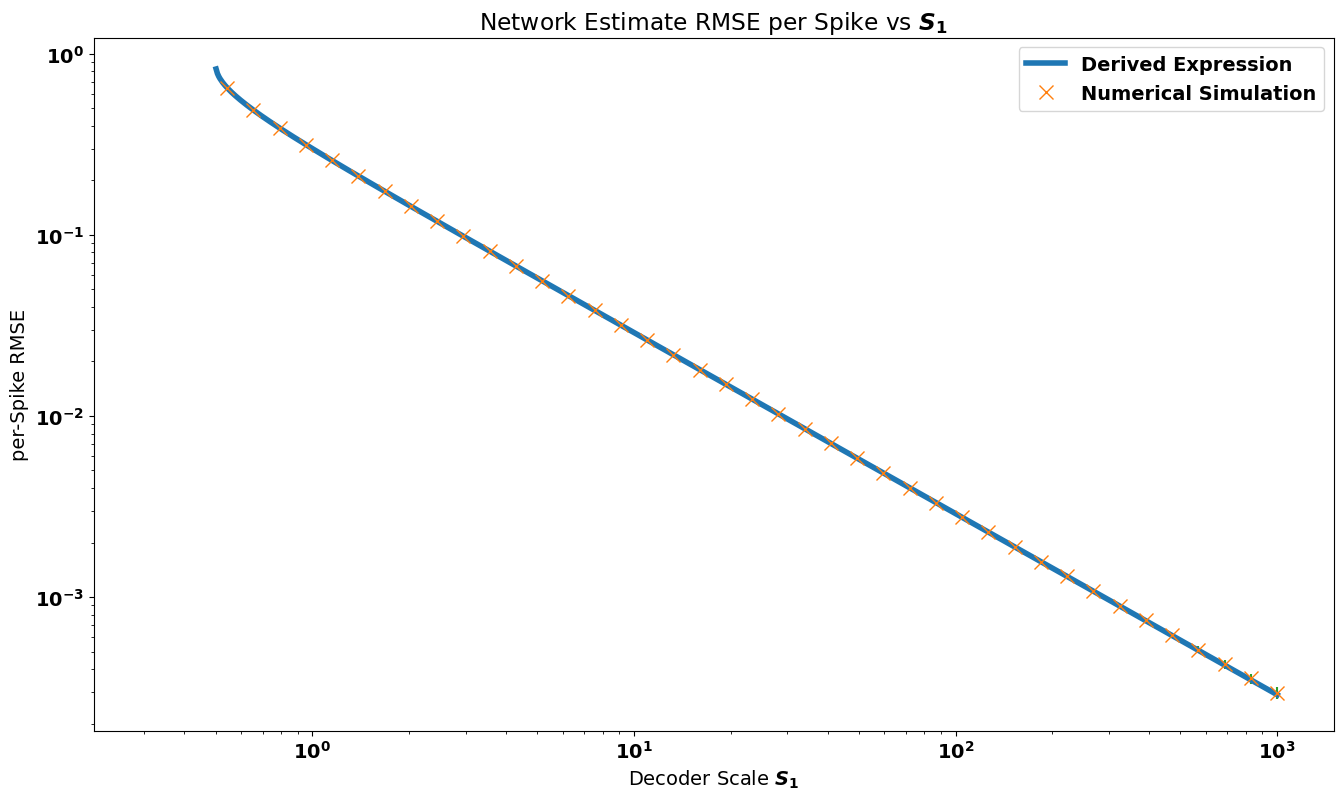
\includegraphics[width=\linewidth]{figures/rmse_sp_vs_s_const_driving.png}
\centering
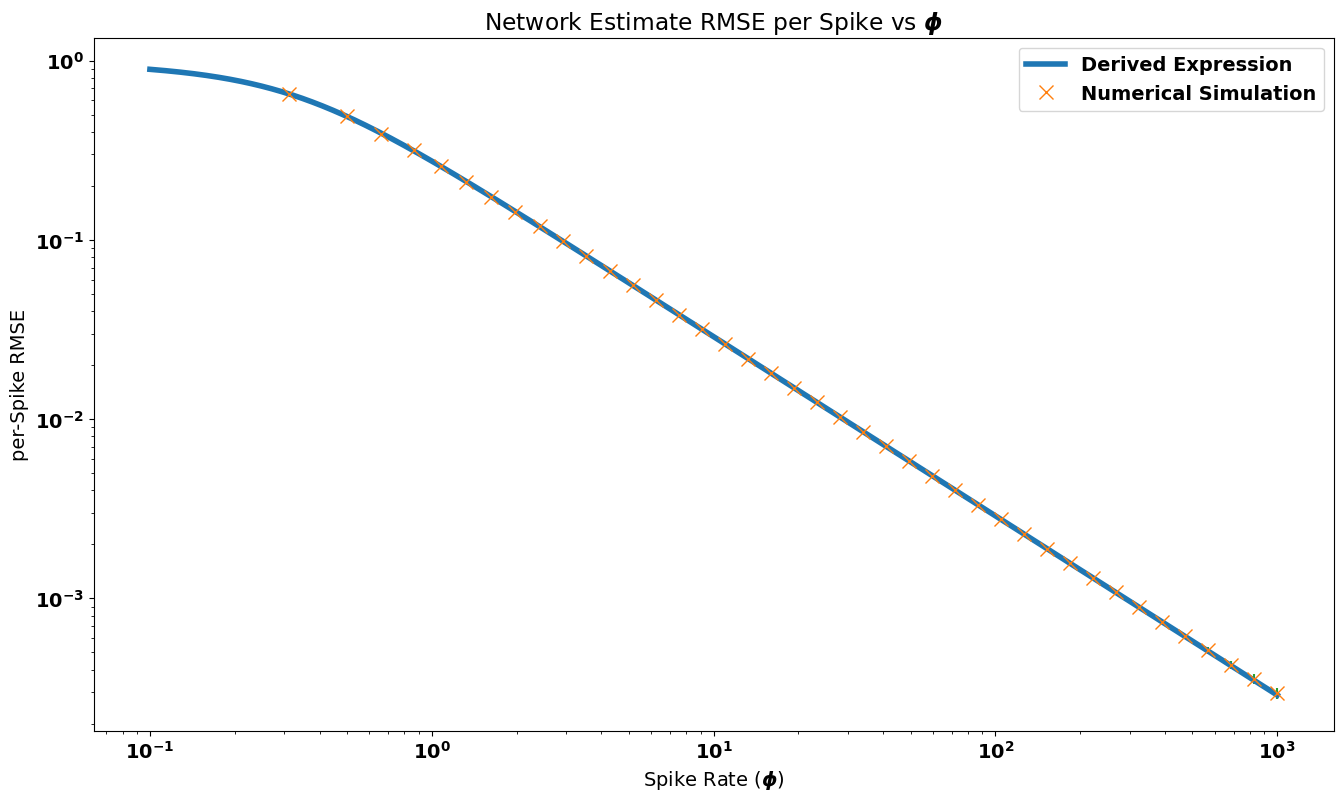
\includegraphics[width=\linewidth]{figures/rmse_sp_vs_phi_s_const_driving.png}
\caption{\textbf{\textit{Top:}} A log-log plot of equation (\ref{eq:analysis:const_dynamics_per_spike_rmse_phi_s}) compared with numerical measurements.  \textbf{\textit{Bottom:}} A log-log plot of equation (\ref{eq:analysis:const_dynamics_per_spike_rmse_phi}).
\textbf{\textit{Both:}} Each simulated data point is the RMSE averaged over all inter-spike intervals in a simulation of length $T = 80 \tau_s$ with $d\xi = 10^{-4}$. Green vertical lines visible towards the larger values are +/- 1 standard deviation over the number of inter-spike intervals in a given simulation. The spike rates $\hat{\phi}$ were computed numerically via dividing the number of spikes in a simulation by the simulation duration. The RMSE between two adjacent spikes was computed by numerical integration as a discrete sum: $\hat{RMSE} = \sqrt{\hat{\phi} \sum_{\tau \text{ between spikes }} e(\xi)^T e(\xi) \, \, d\xi }$.}
\label{fig:analysis:const_dynamics_per_spike_rmse_vs_phi_s}
\end{figure}


 





\end{enumerate}





































\clearpage

\section{Derivation: The Predictive Coding Framework and Gap-Junction Network}


Here we derive the a form of the predictive coding framework (PCF) as defined in Boerlin \& Deneve, 2013. We note an assumption in this model that we later show leads to errant behavior in the network estimate. The correction of this assumption produces an intermittent mode featuring direct membrane voltage coupling. We loosely term this a gap-junction network. We compare the network estimate of all three models (PCF, gap-junction, and self-coupled) for the case of a constant driving stimulus. 

\begin{enumerate}

\item \textbf{\textit{The Predictive Coding Framework (PCF):}} The PCF synthesizes a spiking neural network that implements a given dynamical system. It is briefly derived as follows:\\
\\
Assume the following are given:
\begin{itemize}
    \item A Linear Dynamical System  $\dot{x}(\xi) = A x(\xi) + B c(\xi)$,  $x \in \mathbf{R}^d$
    
    \item A Decoder Matrix $D \in \mathbf{R}^{d\hspace{1mm} x \hspace{1mm}N}$ specifying The tuning curve of N neurons in d-dimensional space. \\
\end{itemize}
Let $o(t) \in \mathbf{R}^{N}$ describe the spike trains whose $j^{th}$ component is given by
\begin{align*}
	o_j(t) \overset{\Delta}{=} \sum_{k=0}^{\infty} \delta(t - t_j^k),
\end{align*} 
where $t_j^k$ is the time of the $k^{th}$ spike of neuron $j$. 
Define the time-varying firing rate of the neurons by 
\begin{align*}
	\frac{d r}{d t}(t) \overset{\Delta}{=} - \tau_s^{-1} r(t) + \tau_s^{-1} o(t),
\end{align*}
where $\tau_s{-1}$ is the decay rate of $r(t)$ given by the inverse synaptic time constant $\tau_s$. For consistency across models, we transform the preceding two equations to dimensionless time via $\xi = \frac{t}{\tau_s} \implies  \tau_s \, d \xi = dt$. This gives
\begin{align}
	\label{eq:analysis:comparison_sc_vs_pcf_vs_gj:pcf_o_def}
	o_j(\xi) \overset{\Delta}{=} \sum_{k=0}^{\infty} \delta(\xi - \xi_j^k),
\end{align}
where $\xi_j^k$ is the $k^{th}$ spike of neuron $j$ in dimensionless time, and
\begin{align*}
	\frac{d r}{d t}(t) &= - \tau_s^{-1} r(t) + \tau_s^{-1}o(t),
	\\
	\\
	\implies
	\frac{d r}{\tau_s \, d \xi}(\xi) &= - \tau_s^{-1} r(\xi) + \tau_s^{-1} o(\xi),
	\\
	\\
	\implies
	\frac{dr}{d\xi}(\xi) &= - r(\xi) + o(\xi).
\end{align*}    
Letting $\dot{\left[ \hspace{5mm} \right]}$ denote differentiation w.r.t. dimensionless time $\xi$, we arrive at 
\begin{align}
\label{eq:analysis:comparison_sc_vs_pcf_vs_gj:pcf_r_def}
\dot{r}(\xi) \overset{\Delta}{=} - r(\xi) + o(\xi). 
\end{align}

The network estimate is defined as 
\begin{align}
\label{eq:analysis:comparison_sc_vs_pcf_vs_gj:pcf_xhat_def}
\hat{x}(\xi) \overset{\Delta}{=} D r(\xi),
\end{align}
which gives rise to the network estimation error
\begin{align}
\label{eq:analysis:comparison_sc_vs_pcf_vs_gj:pcf_error_def}
e(\xi) \overset{\Delta}{=} x(\xi) - \hat{x}(\xi).
\end{align}

The network chooses spike times $\xi_j^k$ to greedily optimize the objective function
\begin{align*}
\mathcal{L}(\xi) = ||x(\xi + d\xi) - \hat{x}(\xi + d\xi)||^2.
\end{align*}
The PCF features regularized rate terms $r(\xi)$ for the sake of biological plausibility. At present we ignore these terms. They only increase the network estimation error $e$ by sacrificing accuracy to minimize $r(\xi)$. 
Using an identical approach to the derivation of the self-coupled network in section (\ref{section:derivation:basic_model}), we arrive at 
\begin{align*}
d_j^T 
\left(
	x - \hat{x}
\right)
&= 
\frac{d_j^T d_j}{2}
\end{align*}
where $d_j$ is the $j^{th}$ column of $D$. We define membrane voltage to get the spiking condition:
\begin{align}
\label{eq:analysis:comparison_sc_vs_pcf_vs_gj:pcf_voltage_def}
v_j &\overset{\Delta}{=} d_j^T (x - \hat{x}) 
\notag
\\
\\
\notag
\implies
d_j^T e &= v_{th}, 
\end{align}

where $v^{th} = \frac{d_j^T d_j}{2}$.

Deriving the dynamics, the preceding equation defines voltage, which in matrix form is given by
\begin{align*}
V &= D^T 
\left(
	x - \hat{x}
\right)
%
\\
\\
%
\implies
\dot{V}
&= 
D^T \dot{x} - D^T \dot{\hat{x}}
&
\\
\\
%
&= D^T 
\left(
	A x + B c
\right)
 - D^T 
 \left(
 D \dot{r}
 \right)
 %
 \\
 \\
 %
 &= 
 D^T A x
 + D^T B c
 - D^T D
\left(
	-r + o 
\right) 
 .
\end{align*}
The PCF makes the assumption that when the network performs correctly, $x = \hat{x}$. We later quantify the estimation error introduced by this assumption and correct it to form the gap-junction model. For now make the assumed substitution $x = \hat{x} = Dr$. 

\begin{align*}
\dot{V} &= D^T A \left(D r\right) + D^T B c + D^T D r - D^T D o
%
\\
\\
%
&= 
D^T
\left(
	A + I 
\right)
 D r
+
D^T B c 
- D^T D o. 
\end{align*}

The model is finalized by the addition of a voltage leakage term to ensure stability, giving the final dynamics equation

\begin{align}
\label{eq:analysis:comparison_sc_vs_pcf_vs_gj:pcf_voltage_dynamics}
\dot{V} = -v
+ D^T 
\left(
A + I
\right)
D r
+ 
D^T B c
- D^T D o.
\end{align}

Equation (\ref{eq:analysis:comparison_sc_vs_pcf_vs_gj:pcf_voltage_dynamics}) scales the spike train $o_j$ by $d_j^T d_j$. Thus the spiking behavior is described by
\begin{align}
\label{eq:analysis:comparison_sc_vs_pcf_vs_gj:pcf_spiking_behavior}
    &v_{th} = \frac{ d_j^T d_j }{2} \notag \\
    \notag \\
    &\text{if  } v_j > v^{th}_j,\notag \\
    \\
    &\text{then  } v_j^{'} = v_j - d_j^T d_j \int \delta(\tau)  \, d\tau ,\notag \\
    \notag \\ 
    &\text{and  } r_j^{'} = r_j + \int \delta(\tau)  \, d\tau \notag.
\end{align}
Equations (\ref{eq:analysis:comparison_sc_vs_pcf_vs_gj:pcf_voltage_dynamics}) and (\ref{eq:analysis:comparison_sc_vs_pcf_vs_gj:pcf_spiking_behavior}) specify the PCF model we compare against. Figure (\ref{fig:analysis:comparison_sc_vs_pcf_vs_gj:pcf_network_decode_demo}) shows simulations of the PCF model with the following parameters:

\begin{align}
\label{eq:analysis:comparison_sc_vs_pcf_vs_gj:pcf_demo_sim_params}
A &= -\begin{bmatrix}  
1 & 0 \\
0 & 1
\end{bmatrix},\notag \\
\notag \\
B &= \begin{bmatrix}  
1 & 0 \\
0 & 1
\end{bmatrix}, \notag \\
\notag \\
c(\xi) &= 10 \begin{bmatrix} 
cos(\frac{\pi}{2} \xi)\\
sin(\frac{\pi}{2} \xi)
\end{bmatrix} + 8 \\
\notag \\
D_{\text{ij}} &\sim  \mathcal{N} (0, 1) \text{ Columns Normalized to Unit Length} \notag \\
\notag \\
d\xi &= 10^{-5}, \notag \\
\notag \\
N &= 32,\notag \\
\notag \\
x(0) &= \begin{bmatrix} \frac{1}{2} & \frac{1}{2} \end{bmatrix}.\notag 
\end{align}\\



% Simulate PCF model here, display error vs time for long-term evolution, highlight this divergence
\begin{figure}
\centering
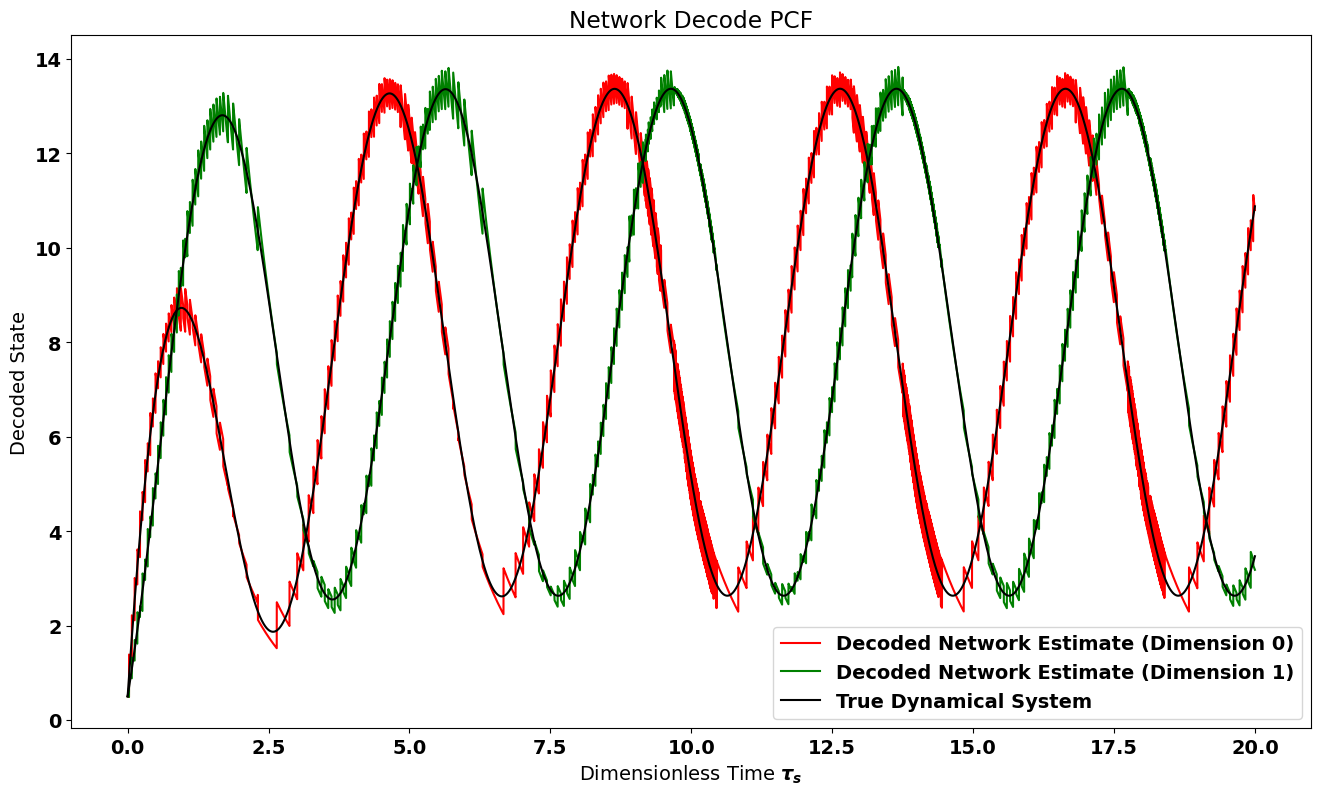
\includegraphics[width=\linewidth]{figures/network_decode_PCF.png}
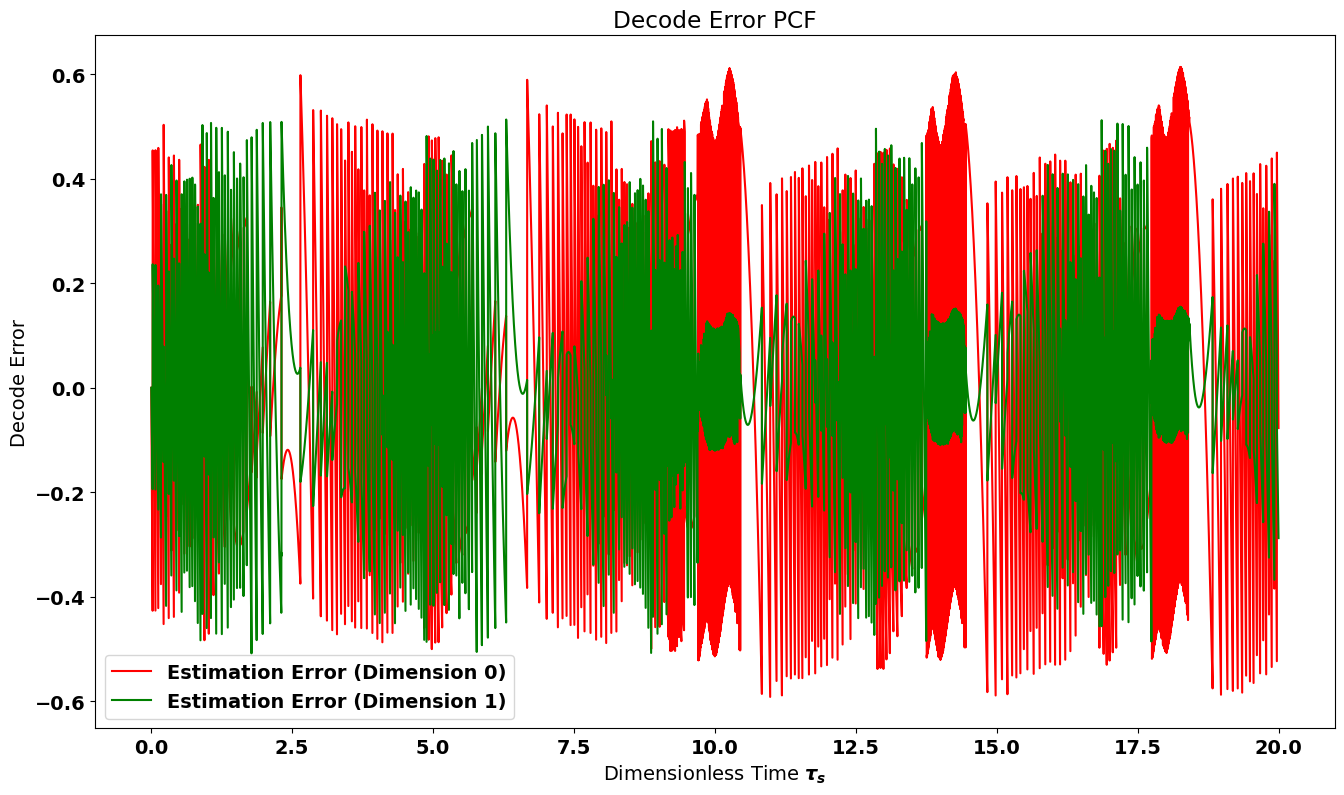
\includegraphics[width=\linewidth]{figures/decode_error_PCF.png}
\caption{Simulation of PCF model given by equations (\ref{eq:analysis:comparison_sc_vs_pcf_vs_gj:pcf_spiking_behavior}) and (\ref{eq:analysis:comparison_sc_vs_pcf_vs_gj:pcf_voltage_dynamics}). \textbf{\textit{Top:}} Network estimate given by equation (\ref{eq:analysis:comparison_sc_vs_pcf_vs_gj:pcf_xhat_def}). \textbf{\textit{Bottom:}} Estimation Error for PCF network from equation (\ref{eq:analysis:comparison_sc_vs_pcf_vs_gj:pcf_error_def}). The simulation parameters are given in equation (\ref{eq:analysis:comparison_sc_vs_pcf_vs_gj:pcf_demo_sim_params}). The numerical implementation is identical to that in section (\ref{section:derivation:basic_model}). A Pad\'e approximation is used to compute a matrix exponential, then used to integrate the continuous terms of the differential equations. The spikes are handled separately at each time step by manually changing the values of neurons above threshold.  For reasons of numerical stability, only one spike per time-step is allowed in the PCF model.  
}
\label{fig:analysis:comparison_sc_vs_pcf_vs_gj:pcf_network_decode_demo}
\end{figure}

\clearpage

\item 
\textbf{\textit{The Gap-Junction Correction:}} Here we correct the assumption that $\hat{x} = x$ made in the PCF model. We restart the previous derivation from this point and derive more a accurate form of equation (\ref{eq:analysis:comparison_sc_vs_pcf_vs_gj:pcf_voltage_dynamics}) termed the gap-junction model.\\
The derivation is identical as the PCF until we derive the voltage dynamics.

\begin{align*}
\dot{V} &= 
D^T A x
+
D^T B c
+ D^T D r
- D^T D o.
\end{align*}
Instead of assuming $x = \hat{x}$, we apply the definition of voltage, equation (\ref{eq:analysis:comparison_sc_vs_pcf_vs_gj:pcf_voltage_def}) in matrix form.
\begin{align*}
v_j &= d_j^T e 
%
\\
\\
%
\implies 
V &= D^T e
%
\\
\\
%
&= 
D^T 
\left(
x - \hat{x}
\right)
%
\\
\\
%
\implies
x 
&=
D^{T \dagger} V  + \hat{x}
%
\\
\\
%
&=
D^{T \dagger} V + D r,
\end{align*}
where $D^{T \dagger}$ is the left Moore-Penrose pseudo-inverse of $D^T$.
Substitute this for $x$ in $\dot{V}$ above to get
\begin{align}
\label{eq:analysis:comparison_sc_vs_pcf_vs_gj:gj_voltage_dynamics}
\dot{V} &= 
D^T A
\left(
	D^{T \dagger} V + D r
\right)
+ D^T D r
+
D^T B c
- D^T D o 
\notag
% 
\\ \notag
\\ 
%
\implies
\dot{V}
&= 
D^T A
D^{T \dagger} V 
+
D^T
\left(
	A + I 
\right)
D r
+ 
D^T B c
- D^T D o.
\end{align}

Equation (\ref{eq:analysis:comparison_sc_vs_pcf_vs_gj:gj_voltage_dynamics}) in conjunction with an identical spiking rule from PCF, equation (\ref{eq:analysis:comparison_sc_vs_pcf_vs_gj:pcf_spiking_behavior}) specifies the gap-junction model. It is simulated in figure (\ref{fig:analysis:comparison_sc_vs_pcf_vs_gj:gj_network_decode_demo}). While the two simulations are similar, there are noticeable differences in their behavior e.g. $\tau_s \simeq 10, \, 13$. 

\begin{figure}
\centering
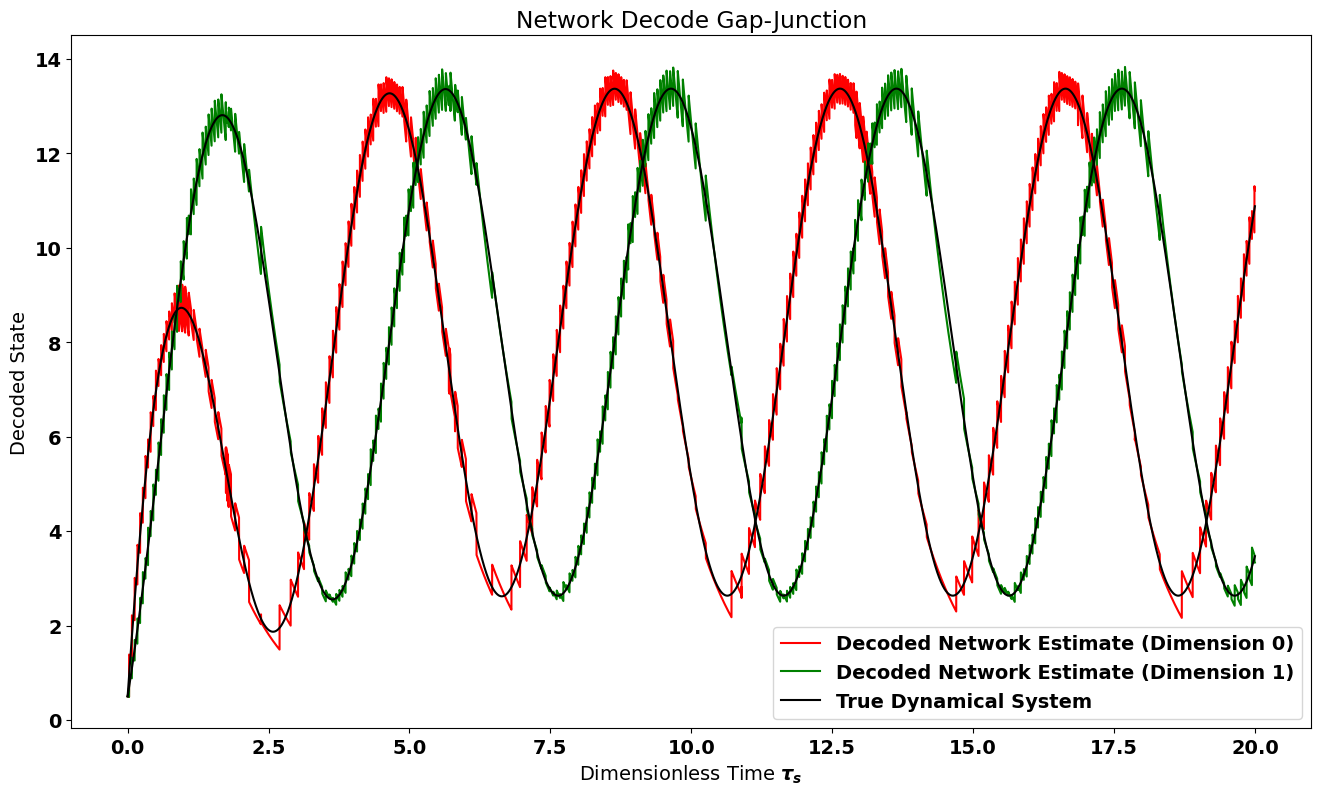
\includegraphics[width=\linewidth]{figures/network_decode_Gap-Junction.png}
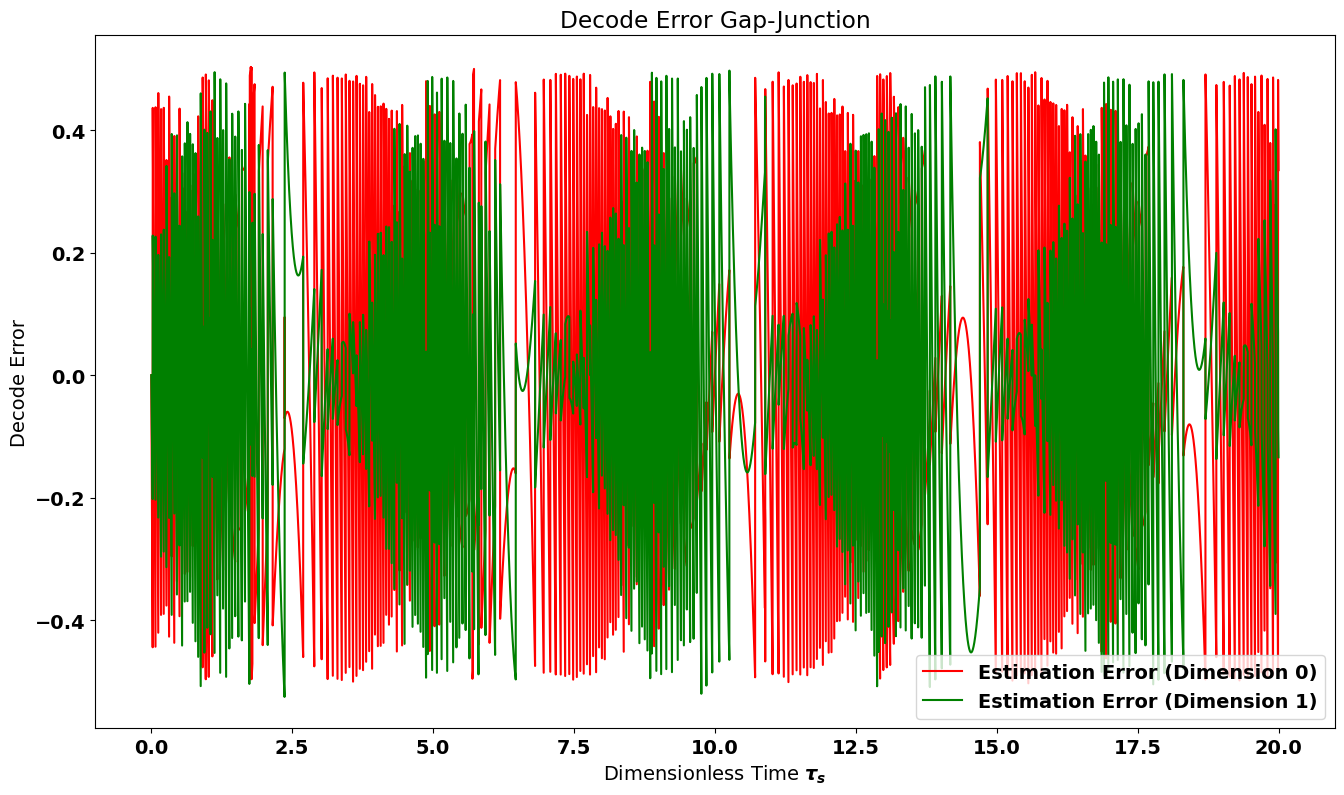
\includegraphics[width=\linewidth]{figures/decode_error_Gap-Junction.png}
\caption{Simulation of the Gap-Junction model given by equations (\ref{eq:analysis:comparison_sc_vs_pcf_vs_gj:pcf_spiking_behavior}) and (\ref{eq:analysis:comparison_sc_vs_pcf_vs_gj:gj_voltage_dynamics}). \textbf{\textit{Top:}} Network estimate given by equation (\ref{eq:analysis:comparison_sc_vs_pcf_vs_gj:pcf_xhat_def}). \textbf{\textit{Bottom:}} Estimation Error for the Gap-Junction network from equation (\ref{eq:analysis:comparison_sc_vs_pcf_vs_gj:pcf_error_def}). The simulation parameters are the same as the previous figure. As with the PCF model, the network is only numerically stable if spikes are restricted to one per time step. 
}
\label{fig:analysis:comparison_sc_vs_pcf_vs_gj:gj_network_decode_demo}
\end{figure}


%The PCF and gap-junction models differ only in their voltage dynamics equations, (\ref{eq:analysis:comparison_sc_vs_pcf_vs_gj:pcf_voltage_dynamics}) and (\ref{eq:analysis:comparison_sc_vs_pcf_vs_gj:gj_voltage_dynamics}) respectively. Suppose we use both models to simulate a target dynamical system. Denote the estimate of the PCF network as $\hat{x}_{pcf}$, and the estimate of the gap-junction network as $\hat{x}_{gj}$. We wish to derive the difference between these estimates denoted by $\chi$. 
%\begin{align}
%	\label{eq:analysis:comparison_sc_vs_pcf_vs_gj:pcf_vs_gj_estimation_error_def}
%	\chi \hspace{2mm} \overset{\Delta}{=} \hspace{2mm} \hat{x}_{pcf} - \hat{x}_{gj}.
%\end{align}
%
%To compute $\chi$, invert our voltage definition equation (\ref{eq:analysis:comparison_sc_vs_pcf_vs_gj:pcf_voltage_def}) in matrix form to get
%\begin{align*}
%V
%&= 
%D^T
%\left(
%	x - \hat{x}
%\right)
%%
%\\
%\\
%%
%\implies 
%\hat{x}
%&= 
%x - D^{T \dagger} V
%%
%\\
%\\
%%
%\implies
%\hat{x}_{pcf} - \hat{x}_{gj}
%&= 
%\chi
%%
%\\
%\\
%%
%&= 
%D^{T \dagger} 
%\left(
%	V_{gj} - V_{pcf}
%\right)
%%
%\\
%\\
%%
%\implies 
%\dot{\chi} 
%&= 
%D^{T \dagger} 
%\left(
%	\dot{V}_{gj} -
%	\dot{V}_{pcf}
%\right). 
%\end{align*}
%
%
%Subtract the right hand sides of equation (\ref{eq:analysis:comparison_sc_vs_pcf_vs_gj:pcf_voltage_dynamics})from (\ref{eq:analysis:comparison_sc_vs_pcf_vs_gj:gj_voltage_dynamics}) to get
%
%\begin{align*}
%\dot{V}_{gj} - \dot{V}_{pcf} 
%&=
%D^T A
%D^{T \dagger} V_{gj} + V_{pcf}
%%
%\\
%\\
%%
%\implies
%\dot{\chi}
%&=
%A D^{T \dagger} V_{gj}
%+ 
%D^{T \dagger} V_{pcf}
%%
%\\
%\\
%%
%&= 
%A D^{T \dagger} V_{gj}
%+ 
%D^{T \dagger} V_{pcf}
%-
%A D^{T \dagger} V_{pcf}
%+
%A D^{T \dagger} V_{pcf}
%-
%D^{T \dagger} V_{gj}
%+
%D^{T \dagger} V_{gj}
%%
%\\
%\\
%%
%&= 
%A D^{T \dagger} 
%\left(
%	V_{gj} - V_{pcf}
%\right)
%+ A D^{T \dagger}  V_{pcf}
%+ 
%D^{T \dagger} 
%\left(
%	V_S{pcf} - V_{gj}
%\right)
%+
%D^{T \dagger} V_{gj}
%%
%\\
%\\
%%
%&=
%\left(
%	A - I
%\right)
%\chi
%+ 
%A D^{T \dagger}  V_{pcf}
%+
%D^{T \dagger} V_{gj}
%\end{align*}

\clearpage

\end{enumerate}


\clearpage

\section{Analysis: PCF  and Gap-Junction Response to Constant Stimulus}

 We compare the network estimate of all three models (PCF, gap-junction, and self-coupled) for the case of a constant driving stimulus. 
 
 Let all 3 models have the same parameters as given by equation (\ref{eq:analysis:comparison_sc_vs_pcf_vs_gj:pcf_demo_sim_params}) with the exception that 

\begin{align*}
	c(\xi) &= c = 
	\begin{bmatrix}
		1 \\ 0	
	\end{bmatrix}, 
\end{align*}
and
$x(0) = \begin{bmatrix} \frac{1}{2} & 0 \end{bmatrix}$. 
 
 \subsection{PCF Network Response to Constant Stimulus:}

From equation (\ref{eq:analysis:comparison_sc_vs_pcf_vs_gj:pcf_voltage_dynamics}), the PCF dynamics become
\begin{align*}
	\dot{V}_{pcf}
	&=
	- V_{pcf}
	+
	D^T 
	\left(
		-I + I
	\right)
	D^T r
	+
	D^T 
	\begin{bmatrix}
		1 \\ 0
	\end{bmatrix}
	-
	D^T D o
	%
	\\
	\\
	%
	&= 
	-V_{pcf}
	+ 
	D^T 
	\begin{bmatrix}
		1 \\ 0
	\end{bmatrix}
	-
	D^T D o.
\end{align*}
All voltages are initially 0. From equation (\ref{eq:analysis:comparison_sc_vs_pcf_vs_gj:pcf_spiking_behavior}) the thresholds are identically $\frac{1}{2}$. Until the first spike, neuron $j$'s voltage integrates the quantity $d_j^T 	\begin{bmatrix}	1 \\ 0	\end{bmatrix}$. Denote the neuron $j$ whose tuning curve $d_j$ is closest in angle to $c$ by 

\begin{align*}
	j_{max} \overset{\Delta}{=}
	 \underset{
	 	i \in 
	 	\left[
	 		1, \ldots, N
	 	\right]
	 }
	 {argmax}
	 \hspace{4mm}
	 	d_j^T c.
\end{align*}
Neuron $j_{max}$ will receive the highest driving force and will therefore reach its threshold  before any other neuron. It will then be reset by $1$ to $- \frac{1}{2}$. Each other neuron $k$ will also be reset (decremented) by $d_k^T d_{j_{max}}$, proportional to their angle relative to both neuron $j_{max}$ and the driving strength $c$. This sequence will repeat periodically so that only neuron $j_{max}$ fires at a constant rate. 

We write the PCF network as the one-dimensional equation

\begin{align*}
	v_{pcf} &= 
	- v_{pcf}
	+ d_{j_{max}}^T c 
	- o_{j_{max}}.
\end{align*}

This is a form of the leaky integrate-and-fire (LIF) model, with drive term $d_j^T c(\xi)$. The neuron is driven by inner product $d_{j_{max}}^T c$. Note from equation (\ref{eq:analysis:comparison_sc_vs_pcf_vs_gj:pcf_spiking_behavior}) that the threshold voltage varies with $||d_{j_{max}}||^2$.  For clarity, we drop the subscripts $j$, $j_{max}$ in the following equations. It is understood that we are referring to the solely spiking neuron $j_{max}$.
With initial condition $v_{pcf}(0) = - \frac{||d||^2}{2}$, the neuron's trajectory is integrated as 
\begin{align}
\label{eq:analysis:comparison_sc_vs_pcf_vs_gj:const_stim:pcf_voltage_trajectory}
	v_{pcf}(\xi)
	&= 
	d^T c - e^{-\xi} 
	\left(
		d^T c + \frac{||d||^2}{2}
	\right). 
\end{align}

The neuron spikes when it reaches the threshold $v_{pcf} = ||d||^2$. To compare with the self-coupled network, we note that the singular value associated with neuron $j$ of the decoder matrix $S = ||d||^2$.

From the preceding equation with voltage at  threshold $\frac{||d||^2}{2}$,
\begin{align*}
	\frac{||d||^2}{2}
	&= 
	d^T c - e^{-\xi_{spike}} 
	\left(
		d^T c + \frac{||d||^2}{2}
	\right)
	%
	\\
	\\
	%
	\implies
	e^{-\xi_{spike}}
	&= 
		\frac
	{
		d^T c - \frac{||d||^2}{2}
	}
	{
		d^T c + \frac{||d||^2}{2}
	}
	%
	\\
	\\
	%
	\implies
	\xi_{spike}
	&= 
	ln
	\left(
		d^T c + \frac{||d||^2}{2}
	\right)
	-
	ln
	\left(
		d^T c - \frac{||d||^2}{2}
	\right)		
\end{align*}
This leads to a firing rate 

\begin{align}
\label{eq:analysis:comparison_sc_vs_pcf_vs_gj:const_dynamics:pcf_spike_rate}
	\phi_{pcf}
	\left(
		d
	\right)
	 =
	 \frac
	 {
	 	1
	 }
	 {
		ln
		\left(
			d^T c + \frac{||d||^2}{2}
		\right)
		-
		ln
		\left(
			d^T c - \frac{||d||^2}{2}
		\right)		
	}
\end{align}

Deriving the network estimate, suppose it begins at $x(0)$. The trajectory until the first spike at time $\xi_1$ is
$$
\hat{x}(\xi) = x(0) e^{-\xi}, \hspace{4mm} 0 \leq \xi < \xi_1.
$$

The spike adds $d$ to the readout followed by exponential decay:
$$
\hat{x}(\xi) =
\left(
	x(0) e^{-\xi_1}
    +
	d
\right)
 e^{-(\xi-\xi_1)} , \hspace{4mm} 0 \leq \xi-\xi_1 < \frac{1}{\phi}.
$$
Until the third spike the readout is
$$
\hat{x}(\xi) =
\left(
	x(0) e^{-\xi_1} e^{-\frac{1}{\phi} }
    +
	d e^{-\frac{1}{\phi}}
	+ d
\right)
 e^{-(\xi - \frac{1}{\phi} - \xi_1)}
	 , \hspace{4mm} \frac{1}{\phi} \leq \xi-\xi_1 < \frac{2}{\phi}.
$$
The recursive pattern is visible after the third spike
$$
\hat{x}(\xi) =
\left(
	x(0) e^{-\xi_1} e^{-\frac{2}{\phi} }
    +
	d e^{-\frac{2}{\phi}}
	+ d e^{-\frac{1}{\phi}}
	+d
\right)
 e^{-(\xi - \frac{2}{\phi} - \xi_1)}
	 , \hspace{4mm} \frac{2}{\phi} \leq \xi-\xi_1 < \frac{3}{\phi}.
$$

Consider the $n^{th}$ term for $n$ big enough so that the $x(0)$ term is approximately $0$. The readout at spike time $\xi_n$ is given by the sum
$$
\hat{x}(\xi_n) =  d \sum_{l = 0}^{n-1} e^{-\frac{l}{\phi}}.
$$
The series converges to 
$$
\hat{x}(\xi_n) =  
\frac
{
	d
}
{
	1 - e^{-\frac{1}{\phi}}.
}
$$
Between the spikes the readout exponentially decays so that the network estimate is given by

\begin{align}
\label{eq:analysis:comparison_sc_vs_pcf_vs_gj:const_dynamics:pcf_network_estimate_steady_state}
\hat{x}_{pcf}(\xi) =
\frac
{
	d
}
{
	1 - e^{-\frac{1}{\phi}}
}
e^
{
	- \hspace{2mm}
	\left(
		\xi - \xi_1^1
	\right)
	\mod
	{
		\frac
		{
			1
		}
		{
			\phi
		}
	}
}.
\end{align}


\subsection{Gap-Junction Network Response to Constant Stimulus:} Here we derive the decoded estimate of a gap-junction network driven by a constant stimulus, $c(\xi) = \begin{bmatrix}
1 & 0
\end{bmatrix}
$. All other parameters are identical to those in equation (\ref{eq:analysis:comparison_sc_vs_pcf_vs_gj:pcf_demo_sim_params}).

From the dynamics equation (\ref{eq:analysis:comparison_sc_vs_pcf_vs_gj:gj_voltage_dynamics}) gap-junction voltages are continuously coupled to one another via $D^T A D^{T \dagger}$. We thus need to solve the entire system between spikes rather than reducing it to a single dimension. Let $\tilde{[]}$ denote the Laplace transform of a variable. Assume neuron j has just spiked so that 

\begin{align*}
V(0) = -\frac{1}{2}
\begin{bmatrix}
d_1 ^T d_j
\\
\vdots
\\
d_j^T d_j
\\
\vdots
\\
d_N^T d_j
\end{bmatrix}.
\end{align*}

Since $c(\xi) = \begin{bmatrix}
1 \\ 0
\end{bmatrix}$, $B = I$, and $o(\xi) = 0$ between spikes, we have

$$
	\dot{V} 
	=
	D^T A D^{T \dagger} V
	+ 
	D^T 
	\left(
		A + I
	\right)
	D r
	+
	d_1,
$$
where $d_1$ is the first column of $D$. 
Apply the one-sided Laplace Transform to both sides and use the Laplace derivative property:
\begin{align*}
	s \tilde{V} - V(0)
	&=
	D^T A D^{T \dagger} \tilde{V}
	+
	D^T 
	\left(
		A + I
	\right)o
	D \tilde{r}
	+
	\mathcal{L}\left[d_1\right]
	%
	\\
	\\
	%
	\implies
	\left(
	s \, I - D^T A D^{T \dagger} 
	\right)
	\tilde{V}
	&=
	V(0)
	+
		D^T 
	\left(
		A + I
	\right)
	D \tilde{r}
	+
	\tilde{d_1}	
	%
	\\
	\\
	%
	\implies 
	\tilde{V}
	&= 
	\left(
	s \, I - D^T A D^{T \dagger} 
	\right)^{-1}
	\left[
		V(0)
		+
		D^T 
		\left(
			A + I
		\right)
		D \tilde{r}
		+
		\tilde{d_1}	
	\right]
	%
	\\
	\\
	%
	&= 
	\left(
		sI - D^T A D^{T \dagger}
	\right)^{-1}
	V(0)
	+ 
		\left(
		sI - D^T A D^{T \dagger}
	\right)^{-1}
	D^T 
	\left(
		A + I
	\right)	
	D \tilde{r}
	+
	\tilde(d_1).
\end{align*}

Now apply the inverse Laplace transform. Note that by definition of matrix exponential, 

$$
	\mathcal{L}^{-1} 
	\left(
		sI - D^T A D^{T \dagger}
	\right)^{-1}
	= e^{\xi D^T A D^{T \dagger}}.
$$
Therefore, 
\begin{multline}
\label{eq:analysis:comparison_sc_vs_pcf_vs_gj:gj_voltage_intermittent_laplace_transformed}
	V(\xi)
	=
	e^{\xi D^T A D^{T \dagger}} V(0)
	+
	\mathcal{L}^{-1}
	\left[
		\left(
			sI - D^T A D^{T \dagger}
		\right)^{-1}
		D^T B \tilde{c}
	\right]
	\\
		+ 
	\mathcal{L}^{-1}
	\left[
		\left(
			sI - D^T A D^{T \dagger}
		\right)^{-1}
		D^T 
		\left(
			A + I
		\right)	
		D \tilde{r}
	\right].
\end{multline}
\\
To simplify the second term of equation (\ref{eq:analysis:comparison_sc_vs_pcf_vs_gj:gj_voltage_intermittent_laplace_transformed}), use the convolution-product property of the Laplace transform to get
\\
$$
	\mathcal{L}^{-1}
	\left[
		\left(
			sI - D^T A D^{T \dagger}
		\right)^{-1}
		D^T B \tilde{c}
	\right]
	=
	\mathcal{L}^{-1}
	\left[
			\left(
			sI - D^T A D^{T \dagger}
		\right)^{-1}		
	\right]
	\,	* \, 
		\mathcal{L}^{-1}
	\left[
			D^T B \tilde{c}
	\right].
$$
\\
Note $c(\xi) = \begin{bmatrix}
1 \\ 0
\end{bmatrix}$, and $B = I$. Therefore,
\\
$$
		\mathcal{L}^{-1}
	\left[
			D^T B \tilde{c}
	\right] = D^T B c = d_1,
$$\\
where $d_1$ is the first column of $D$.
The entire second term in  $V(\xi)$ above becomes

$$
	\mathcal{L}^{-1}
	\left[
		\left(
			sI - D^T A D^{T \dagger}
		\right)^{-1}
		D^T B \tilde{c}
	\right]
	=
	e^{\xi D^T A D^{T \dagger}} * d_1.
$$
\\
Evaluating the convolution, bring $d_1$ outside the integral, a linear operator:
$$
	e^{\xi D^T A D^{T \dagger}} * d_1 (\xi)
	=
	\int_{\tau=-\infty}^{\infty}
		e^{
		\left(
			\xi - \tau
		\right)
		 D^T A D^{T \dagger}} 
	\, d\tau
	 \, d_1.
$$
\\
The state $V(\xi)$ depends only on the past up to $V(0)$ so that $0 < \xi - \tau \leq  \xi$: 
\\
$$
	e^{\xi D^T A D^{T \dagger}} * d_1 (\xi)
	=
	\int_{\tau=0}^{\xi}
		e^{
		\left(
			\xi - \tau
		\right)
		 D^T A D^{T \dagger}}  
	\, d\tau
	\, d_1.
$$
\\
The integral of the matrix exponential $\int_{t=0}^{T} \, e^{tX} \, dt= X^{-1} \left(e^{Tx} - I \right)$. Thus,
\\
\begin{equation}
\label{eq:analysis:comparison_sc_vs_pcf_vs_gj:gj_voltage_intermittent_laplace_transformed_term_2}
	\mathcal{L}^{-1}
	\left[
		\left(
			sI - D^T A D^{T \dagger}
		\right)^{-1}
		D^T B \tilde{c}
	\right]
=
\left(
	D^T A D^{T \dagger}
\right)^{-1}
\left(
	e^{\xi D^T A D^{T \dagger}} - I
\right)
d.
\end{equation}

Note the notation $d = D^T B c$. 
Looking at the final term of equation (\ref{eq:analysis:comparison_sc_vs_pcf_vs_gj:gj_voltage_intermittent_laplace_transformed}), assume the network estimate is periodic with period $\frac{1}{\phi}$, where $\phi$ is the unknown spike rate. Between spikes, the dynamics of $r(\xi)$ are known from equation (\ref{eq:analysis:comparison_sc_vs_pcf_vs_gj:pcf_r_def}) solved as
$$
	r(\xi) = e^{-\xi I} r(0), \hspace{4mm} 0 < \xi \leq  \frac{1}{\phi}.
$$
Hence, 
\begin{align*}
	\mathcal{L}^{-1}
	\left[
		\left(
			sI - D^T A D^{T \dagger}
		\right)^{-1}
		D^T 
		\left(
			A + I
		\right)	
		D \tilde{r}
	\right]
	&= 
	\mathcal{L}^{-1}
	\left[
		\left(
			sI - D^T A D^{T \dagger}
		\right)^{-1}		
	\right]
	\, 
	*	
	\,
	\mathcal{L}^{-1}
	\left[
		D^T 
		\left(
			A + I
		\right)	
		D \tilde{r}
	\right]
	%
	\\
	\\
	%
	&=
	e^{\xi D^T A D^{T \dagger}}
	\, 
	*	
	\,
		D^T 
		\left(
			A + I
		\right)	
		D \, 
		e^{-\xi \, I} \, r(0)		
	%
	\\
	\\
	%
	&= 	e^{\xi D^T A D^{T \dagger}}
	\, 
	*	
	\,
	\left(
		D^T A D e^{-\xi \, I} \, r(0)
		+
		D^T D e^{-\xi \, I} \, r(0)
	\right)	
	%
	\\
	\\
	%
	&=
	e^{\xi D^T A D^{T \dagger}}
	\, 	*  \,
	D^T A D e^{-\xi \, I} \, r(0)	
	+
	e^{\xi D^T A D^{T \dagger}}
	\, 	*  \,
	D^T D e^{-\xi \, I} \, r(0).	
\end{align*}

The two convolutions are nearly identical so we solve the simpler of the two:
\\
$$
	e^{\xi D^T A D^{T \dagger}}
	\, 	*  \,
	D^T D e^{-\xi \, I} \, r(0)
	= 
	\int_{\tau=0}^{\xi} \,
		e^{ \left(\xi-\tau\right) D^T A D^{T \dagger}}
		D^T D e^{-\tau \, I} \, r(0)
		\, d\tau.
$$

Note that $e^{-\tau \, I}$ simplifies as 
\begin{align*}
e^{-\tau \, I}
&=
\sum_{k=0}^{\infty}
\frac{\left(-\tau I\right)^{k}}{k!}
%
\\
\\
%
&=
\left(
	\sum_{k=0}^{\infty}
	\frac{(-\tau^{k})}{k!}
\right) I
%
\\
\\
%
&= e^{-\tau} I.
\end{align*}
The scalar and identity matrix can both move to the beginning of the integral and reformed into a matrix:
\begin{align*}
	\int_{\tau=0}^{\xi} \,
		e^{ \left(\xi-\tau\right) D^T A D^{T \dagger}}
		D^T D e^{-\tau \, I} \, r(0)
	\, d\tau
	&= 
	\int_{\tau=0}^{\xi} \,
		e^{-\tau \, I}
		e^{ \left(\xi-\tau\right) D^T A D^{T \dagger}}
		D^T D \, r(0)
	\, d\tau
	%
	\\
	\\
	%
	&=
	e^{\xi D^T A D^{T \dagger}}
	\int_{\tau=0}^{\xi} \,
		e^
		{
			-\tau \, \left( I + D^T A D^{T \dagger} \right)
		}
	\, d\tau
	\, \,
	D^T D \, r(0)
	%
	\\
	\\
	%
	&=
	e^{\xi D^T A D^{T \dagger}}
	\left( I + D^T A D^{T \dagger} \right)^{-1}
	\left(
		e^{\xi \left( I + D^T A D^{T \dagger} \right)} - I
	\right)
	D^T D \, r(0).
\end{align*}

From this expression it follows that 
\\
$$
	e^{\xi D^T A D^{T \dagger}}
	\, 
	*	
	\,
		D^T 
		\left(
			A + I
		\right)	
		D \, 
		e^{-\xi \, I} \, r(0)
	=
		e^{\xi D^T A D^{T \dagger}}
	\left( I + D^T A D^{T \dagger} \right)^{-1}
	\left(
		e^{\xi \left( I + D^T A D^{T \dagger} \right)} - I
	\right)
	D^T(A + I)D \, r(0).	
$$
\\
Hence, 

\begin{align}
\label{eq:analysis:comparison_sc_vs_pcf_vs_gj:gj_voltage_intermittent_laplace_transformed_term_1}
\mathcal{L}^{-1}
	\left[
		\left(
			sI - D^T A D^{T \dagger}
		\right)^{-1}
		D^T 
		\left(
			A + I
		\right)	
		D \tilde{r}
	\right]
	=
	e^{\xi D^T A D^{T \dagger}}
	\left( I + D^T A D^{T \dagger} \right)^{-1}
	\left(
		e^{\xi \left( I + D^T A D^{T \dagger} \right)} - I
	\right)
	D^T(A + I)D \, r(0).	
\end{align}

Using equations (\ref{eq:analysis:comparison_sc_vs_pcf_vs_gj:gj_voltage_intermittent_laplace_transformed_term_2}) and (\ref{eq:analysis:comparison_sc_vs_pcf_vs_gj:gj_voltage_intermittent_laplace_transformed_term_1}), the voltage trajectory equation (\ref{eq:analysis:comparison_sc_vs_pcf_vs_gj:gj_voltage_intermittent_laplace_transformed}) becomes 
\begin{align}
	\label{eq:analysis:comparison_sc_vs_pcf_vs_gj:gj_voltage_solved_full}
	V(\xi)
	= \notag \\ \notag
	& e^{\xi D^T A D^{T \dagger}} V(0)
	\\ \notag
	\\ &+ 
	\left(
		D^T A D^{T \dagger}
	\right)^{-1}
	\left(
		e^{\xi D^T A D^{T \dagger}} - I
	\right)
	d
	\\ \notag
	\\&+ \notag
	e^{\xi D^T A D^{T \dagger}}
	\left( I + D^T A D^{T \dagger} \right)^{-1}
	\left(
		e^{\xi \left( I + D^T A D^{T \dagger} \right)} - I
	\right)
	D^T(A + I)D \, r(0).
\end{align}
\\
In the case $A = -I$, equation (\ref{eq:analysis:comparison_sc_vs_pcf_vs_gj:gj_voltage_solved_full}) simplifies considerably:

\begin{align}	
\label{eq:analysis:comparison_sc_vs_pcf_vs_gj:gj_voltage_solved_simple}
	V(\xi)
	&=
	 e^{-\xi D^T D^{T \dagger}} V(0)
	+
	\left(
		D^T D^{T \dagger}
	\right)^{-1}
	\left(
		I - e^{-\xi D^T D^{T \dagger}}
	\right)
	d.
\end{align}

Simplify the matrix $D^T D^{T \dagger}$ via its SVD:

\begin{align*}
	D^T
	&=
	V \begin{bmatrix} S \\ 0\end{bmatrix} \mathcal{U}^T,
	%
	\\
	\\
	%
	\implies
	D^{T \dagger}
	&= 
	\mathcal{U} \begin{bmatrix} S & 0\end{bmatrix} V^T
	%
	\\
	\\
	%
	\implies 
	D^T D^{T \dagger} 
	&=
	V \begin{bmatrix} S \\ 0\end{bmatrix} \mathcal{U}^T \mathcal{U} \begin{bmatrix} S & 0\end{bmatrix} V^T
	\\
	\\
	&=
	V \begin{bmatrix} S \\ 0\end{bmatrix} \begin{bmatrix} S & 0\end{bmatrix} V^T
	\\
	\\
	&= V \begin{bmatrix} I_{d} & 0 \\ 0 & 0 \end{bmatrix}  V^T
	\\
	\\
	&= \begin{bmatrix} I_{d} & 0 \\ 0 & 0 \end{bmatrix} \in \mathbf{R}^{N \text{ x } N},
\end{align*}
where $I_{d}$ denotes the d-dimensional identity matrix. Equation (\ref{eq:analysis:comparison_sc_vs_pcf_vs_gj:gj_voltage_solved_simple}) becomes
\\
$$
	V(\xi)
	=
	 e^{-\xi I_d } V(0)
	+
	\begin{bmatrix} I_{d} & 0 \\ 0 & 0 \end{bmatrix}^{-1}
	\left(
		I - e^{-\xi I_d}
	\right)
	d.
$$
The matrix $\begin{bmatrix} I_{d} & 0 \\ 0 & 0 \end{bmatrix}$ is not invertible. Consider instead only the first $d$ equations of the preceding system. 

$$
	V_j(\xi)
	=
	 e^{-\xi} V_j(0)
	+
	\left(
		1 - e^{-\xi}
	\right)
	d_j , \hspace{4mm} j = 1, \ldots, d.
$$
Note that $d_j = d^T c$, and consider neuron $j_{max} = j$ the first to reach the spike threshold. Recall its initial condition $v(0) = -\frac{||d||^2}{2}$ to arrive at
$$
	V(\xi)
	=
	 - e^{-\xi} \frac{||d||^2}{2}
	+
	\left(
		1 - e^{-\xi}
	\right)
	d^T c
$$
Compare with the corresponding PCF trajectory, equation (\ref{eq:analysis:comparison_sc_vs_pcf_vs_gj:const_stim:pcf_voltage_trajectory}). The preceding equation rearranges to
$$
	V(\xi) = 
	d^T c 
	- e^{-\xi}
	\left(
		d^T c  + \frac{||d||^2}{2}
	\right),
$$

which is identical to equation (\ref{eq:analysis:comparison_sc_vs_pcf_vs_gj:const_stim:pcf_voltage_trajectory}). Since only one neuron spikes, $r(\xi)$ and thus $\hat{x}(\xi)$ are identical for both PCF and gap-junction networks. 
The preceding, somewhat painful analysis shows that if the PCF and gap-junction models begin on their steady-state trajectories with the same initial conditions, their network estimates are identical in time. The statement is limited to the case of a constant driving stimulus. It does not, for example, show which network reaches the steady state trajectory first.



\subsection{Per-spike RMSE of the PCF and Gap-Junction Networks for a Constant Stimulus}

Equation (\ref{eq:analysis:comparison_sc_vs_pcf_vs_gj:const_dynamics:pcf_network_estimate_steady_state}) gives both gap-junction and PCF trajectories. We compute the per-spike RMSE by the integral 
$$
RMSE_{spike} \overset{\Delta}{=}\
\sqrt
{
	\phi \int_
	{	
		0
	}
	^
	{
		\frac
		{
			1
		}
		{
			\phi
		}
	}
	 \!  e^T e(\tau)\, \, \mathrm{d} \tau
}.
$$
The target dynamical system over this interval is $x(\xi) = \mathcal{U}_1$. Assuming the first spike is at $\xi_1 = 0$, we have 

\begin{align*}
e(\xi) 
&=
x(\xi) - \hat{x}(\xi)
\\
\\
&=
\mathcal{U}_1 
- 
\frac
{
	d
}
{
	1 - e^{-\frac{1}{\phi}}
}
e^{-\xi}
\\
\\
\implies
e^T e &= 
\mathcal{U}_1^T \mathcal{U}_1 
- 2 \, 
\mathcal{U}_1^T \frac
{
	d
}
{
	1 - e^{-\frac{1}{\phi}}
}
e^{-\xi}
+ 
\frac
{
	d^T d
}
{
	\left(1 - e^{-\frac{1}{\phi}}\right)^2
}
e^{- 2 \xi}
\\
\\
&= 
1 - 2 \frac{ c^T d } {1 - e^{-\frac{1}{\phi}}} e^{-\xi}
+ 
\frac
{
	d^T d
}
{
	\left(1 - e^{-\frac{1}{\phi}}\right)^2
}
e^{- 2 \xi}. 
\end{align*}
Integrate over a spike interval to arrive at 

\begin{align*}
 \int_
	{	
		0
	}
	^
	{
		\frac
		{
			1
		}
		{
			\phi
		}
	}
	 \!  e^T e(\tau)\, \, \mathrm{d} \tau
	 &= 
	 \frac{1}{\phi}
	 - 
	 2 \frac{ c^T d } {1 - e^{-\frac{1}{\phi}}}  
	 \left(
	 	1 - e^{-\frac{1}{\phi}}
     \right)
	 + 
	 \frac
	 {
		d^T d
	 }
	 {
		\left(1 - e^{-\frac{1}{\phi}}\right)^2
	 }
	 \frac{1}{2}`
	 \left(
	 	1 - e^{-\frac{2}{\phi}}
     \right)
     \\
     \\
     &= 
	 \frac{1}{\phi}
	 - 
	 2 \,  c^T d 
	 + 
 	 \frac{||d||}{2}
	 \frac
	 {
		1 - e^{-\frac{2}{\phi}}
	 }
	 {
		\left(1 - e^{-\frac{1}{\phi}}\right)^2
	 }.
\end{align*}
The per-spike RMSE of both PCF and Gap-Junction Networks is therefore

\begin{align*}
	RMSE_{spike} = 
	\sqrt{
		1
		-
		2 \, \phi  c^T d 
		 + 
	 	\phi \frac{||d||^2}{2}
		\frac
		{
			1 - e^{-\frac{2}{\phi}}
		}
		{
			\left(1 - e^{-\frac{1}{\phi}}\right)^2
		}
	}.
\end{align*}

To write the RMSE as a function of only firing rate $\phi$, we invert equation (\ref{eq:analysis:comparison_sc_vs_pcf_vs_gj:const_dynamics:pcf_spike_rate}) to obtain $d(\phi)$:
$$
\frac{1}{\phi} = 
ln
\left(
	d^T c + \frac{||d||^2}{2}
\right)
-
ln 
\left(
	d^T c - \frac{||d||^2}{2}
\right). 
$$ 

Note that $d^T c = d^T \begin{bmatrix} 1 \\ 0 \end{bmatrix} = d_0$. Because $d$ is the most parallel vector to $c$, for large enough networks with uniformly distributed directions $d$, we have that $d = d_0  c$. This implies that $||d||^2 = d_0^2$. The preceding equation becomes

\begin{align*}
\frac{1}{\phi} &= 
ln
\left(
	d_0+ \frac{d_0^2}{2}
\right)
-
ln 
\left(
	d_0 - \frac{d_0^2}{2}
\right)
\\
\\
\implies
e^{-\frac{1}{\phi}}
&= 
\frac
{
	d_0 - \frac{d_0^2}{2}
}
{
	d_0 + \frac{d_0^2}{2}
}
\\
\\
&= 
\frac
{
	1 - \frac{d_0}{2}
}
{
	1 + \frac{d_0}{2}
}
\\
\\
\implies
e^{-\frac{1}{\phi}} + e^{-\frac{1}{\phi}} \frac{d_0}{2}
&= 
1 - \frac{d_0}{2}
\\
\\
\implies
d_0
\frac{
1 + e^{-\frac{1}{\phi}} 
}
{2}
&=
1 - e^{-\frac{1}{\phi}}
\\
\\
\implies
d_0(\phi) &=
2\, \frac
{
	1 - e^{-\frac{1}{\phi}}
}
{
	1 + e^{-\frac{1}{\phi}}
}
\\
\\
&= 
2 \, \tanh
{
	\frac{1}{2\phi}
}
\end{align*}

Thus the per-spike RMSE simplifies to 

\begin{align}
\label{eq:analysis:comparison_sc_vs_pcf_vs_gj:per_spike_rmse_pcf_gj}
RMSE_{spike} = 
	\sqrt{
		1
		-
		4 \, \phi  \tanh
{
	\frac{1}{2\phi}
}
		 + 
	 	2 \, \phi
	 	\tanh^2{
	\frac{1}{2\phi}
}
		\frac
		{
			1 - e^{-\frac{2}{\phi}}
		}
		{
			\left(1 - e^{-\frac{1}{\phi}}\right)^2
		}
	}.
\end{align}


\subsection{Comparison of Self-Coupled, Gap-Junction, and PCF Networks for a Constant Stimulus}

We now compare all three models as they respond to a constant driving stimulus, while varying their firing rate. 

Let the parameters be 
\begin{align*}
A &= -
\begin{bmatrix}  
1 & 0 \\
0 & 1
\end{bmatrix},
\\
\\
B &=
\begin{bmatrix}  
	1
	\\
	0 
\end{bmatrix}, 
\\ 
\\
c(\xi) &=  
\begin{bmatrix}  
1  \\
0 \end{bmatrix},
\\
\\
D
&=
\mathcal{U} 
\begin{bmatrix}
S & 0
\end{bmatrix}
V^T
=
\mathcal{U} 
\begin{bmatrix}
I_d & 0
\end{bmatrix}
I_N \notag,
\\
\\
d\xi &= 10^{-4}, \notag \\
\notag \\
N &= 8,\notag \\
\notag \\
x(0) &= \begin{bmatrix} \frac{1}{2} & 0 \end{bmatrix}.
\end{align*}



We simulate the self-coupled, PCF, and gap-junction networks and compare their derived estimates given by equations (\ref{eq:analysis:constant_driving_constant_dynamics_estimate_equation_explicit}) and (\ref{eq:analysis:comparison_sc_vs_pcf_vs_gj:const_dynamics:pcf_network_estimate_steady_state}) respectively. 
Figure (\ref{fig:analysis:comparison_sc_vs_pcf_vs_gj:network_decode_sc_pcf_gj}) shows the network estimates of each model for the above parameters. We see that all trajectories are identical as predicted by our derived estimates, shown by the dotted line. 

\clearpage 

\begin{figure}
\centering
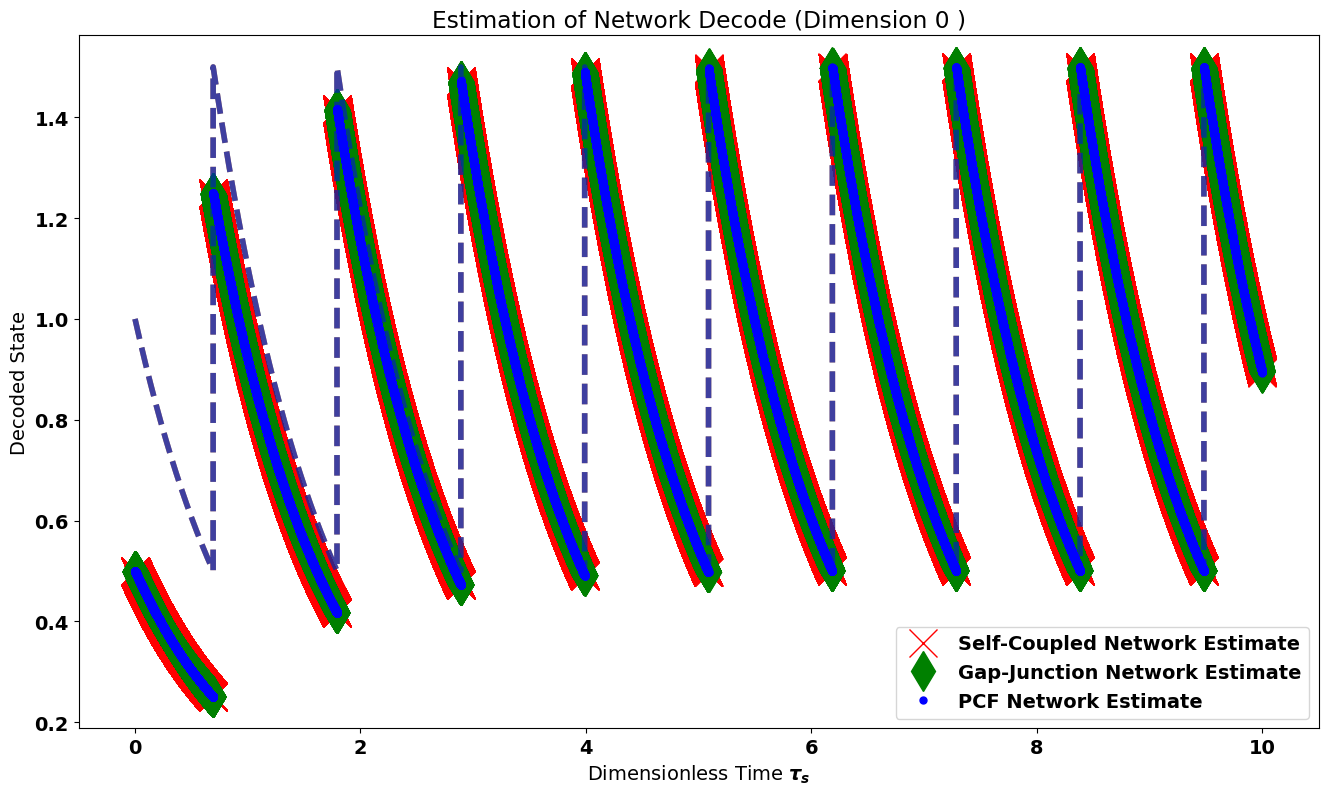
\includegraphics[width=\linewidth]{figures/const_dynamics_network_decode_comparison_sc_pcf_gj}
\caption{Simulation of self-coupled, gap-junction, and PCF networks. Network readouts for each are plotted. The dotted line is the derived expression(s) given by equations (\ref{eq:analysis:constant_driving_constant_dynamics_estimate_equation_explicit}) and (\ref{eq:analysis:comparison_sc_vs_pcf_vs_gj:const_dynamics:pcf_network_estimate_steady_state}). Note that all three trajectories are identical.}
\label{fig:analysis:comparison_sc_vs_pcf_vs_gj:network_decode_sc_pcf_gj}
\end{figure}

Next we plot the per-spike RMSE of each model for the same parameters while varying the spike rate. Figure (\ref{fig:analysis:comparison_sc_vs_pcf_vs_gj:per_spike_rmse_sc_pcf_gj}) shows the numerically measured per-spike RMSE for each model and their derived expressions, equations (\ref{eq:analysis:const_dynamics_per_spike_rmse_phi}) and (\ref{eq:analysis:comparison_sc_vs_pcf_vs_gj:per_spike_rmse_pcf_gj}). As the firing rate approaches the simulation timestep, $10^4$, the curves deviate from the derived expression. 

\begin{figure}
\centering
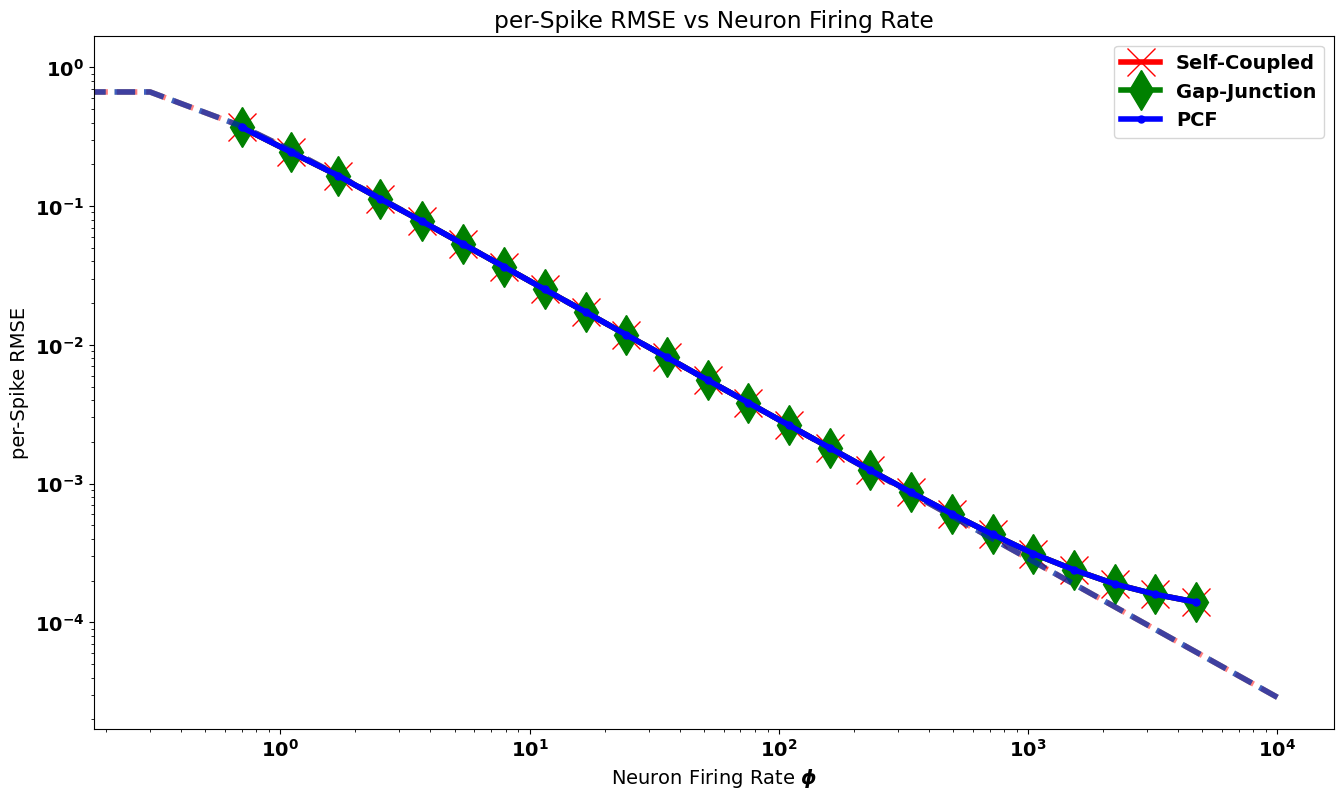
\includegraphics[width=\linewidth]{figures/per_spike_rmse_vs_phi_sc_gj_pcf}
\caption{Simulated per-spike RMSE for self-coupled, gap-junction, and PCF networks. The dotted lines are the derived expression for each model given by given by equations (\ref{eq:analysis:const_dynamics_per_spike_rmse_phi}) for the self-coupled and (\ref{eq:analysis:comparison_sc_vs_pcf_vs_gj:per_spike_rmse_pcf_gj}) for the gap-junction and PCF models respectively. Spike rates were estimated numerically by dividing the number of spikes by the simulation length. The RMSE was computed numerically by the discrete integral $\hat{RMSE} = \sqrt{\hat{\phi} \sum_{\tau \text{ between spikes }} e(\xi)^T e(\xi) \, \, d\xi }$. All computations used the numerically estimated spike rate.} 
\label{fig:analysis:comparison_sc_vs_pcf_vs_gj:per_spike_rmse_sc_pcf_gj}
\end{figure}


\end{document}

